\RequirePackage{silence} % :-\
    \WarningFilter{scrreprt}{Usage of package `titlesec'}
    \WarningFilter{titlesec}{Non standard sectioning command detected}
\documentclass[ twoside,openright,titlepage,numbers=noenddot,headinclude,%1headlines,% letterpaper a4paper
                footinclude=true,cleardoublepage=empty,abstractoff, % <--- obsolete, remove (todo)
                BCOR=5mm,paper=a4,fontsize=11pt,%11pt,a4paper,%
                ngerman,american,dvipsnames
                ]{scrbook}

%********************************************************************
% Note: Make all your adjustments in here
%*******************************************************
% ****************************************************************************************************
% classicthesis-config.tex
% formerly known as loadpackages.sty, classicthesis-ldpkg.sty, and classicthesis-preamble.sty
% Use it at the beginning of your ClassicThesis.tex, or as a LaTeX Preamble
% in your ClassicThesis.{tex,lyx} with \input{classicthesis-config}
% ****************************************************************************************************
% If you like the classicthesis, then I would appreciate a postcard.
% \dfrac{num}{den}y address can be found in the file ClassicThesis.pdf. A collection
% of the postcards I received so far is available online at
% http://postcards.miede.de
% ****************************************************************************************************


% ****************************************************************************************************
% 0. Set the encoding of your files. UTF-8 is the only sensible encoding nowadays. If you can't read
% äöüßáéçèê∂åëæƒÏ€ then change the encoding setting in your editor, not the line below. If your editor
% does not support utf8 use another editor!
% ****************************************************************************************************
\PassOptionsToPackage{utf8}{inputenc}
  \usepackage{inputenc}

% ****************************************************************************************************
% 1. Configure classicthesis for your needs here, e.g., remove "drafting" below
% in order to deactivate the time-stamp on the pages
% (see ClassicThesis.pdf for more information):
% ****************************************************************************************************
\PassOptionsToPackage{
  tocaligned=false, % the left column of the toc will be aligned (no indentation)
  dottedtoc=false,  % page numbers in ToC flushed right
  parts=true,       % use part division
  eulerchapternumbers=true, % use AMS Euler for chapter font (otherwise Palatino)
  linedheaders=true,       % chaper headers will have line above and beneath
  floatperchapter=true,     % numbering per chapter for all floats (i.e., Figure 1.1)
  listings=true,    % load listings package and setup LoL
  subfig=true,      % setup for preloaded subfig package
  eulermath=true,  % use awesome Euler fonts for mathematical formulae (only with pdfLaTeX)
  beramono=true,    % toggle a nice monospaced font (w/ bold)
  minionpro=false   % setup for minion pro font; use minion pro small caps as well (only with pdfLaTeX)
}{tesis}
\usepackage{blindtext}
\usepackage{etoolbox}
\usepackage{algorithm2e}
\usepackage[bottom]{footmisc}
\usepackage{amsfonts}
\usepackage{xr}
\usepackage{amsmath,amsfonts, amssymb, mathrsfs }
\usepackage{tikz-cd}
\usepackage{syntonly}
\usepackage{mathrsfs}
\usepackage{ntheorem}
\PassOptionsToPackage{all}{xy}       % math environments and more by the AMS
	\usepackage{xy}
\PassOptionsToPackage{at}{easylist}       % math environments and more by the AMS
	\usepackage{easylist}
\PassOptionsToPackage{dvipsnames}{xcolor}
	\RequirePackage{xcolor}
\usepackage{upgreek}
% ****************************************************************************************************
% 2. Personal data and user ad-hoc commands
% ****************************************************************************************************
\newcommand{\myTitle}{M\'etodos de primer orden?\xspace}
\newcommand{\mySubtitle}{An\'alisis de convergencia??\xspace}
\newcommand{\myDegree}{Tesis de Licenciatura\xspace}
\newcommand{\myName}{Axel Sirota\xspace}
\newcommand{\myDirector}{Director de Tesis: Dr. Pablo Amster\xspace}
\newcommand{\myFaculty}{Facultad de Ciencias Exactas y Naturales\xspace}
\newcommand{\myDepartment}{Departamento de Matem\'atica\xspace}
\newcommand{\myUni}{Universidad de Buenos Aires\xspace}
\newcommand{\myLocation}{Buenos Aires\xspace}
\newcommand{\myTime}{Septiembre 2018\xspace}
\newcommand{\myVersion}{version 0.1}
\newcommand{\B}{\mathcal{B}}
\newcommand{\Cont}{\mathcal{C}}
\newcommand{\F}{\mathcal{F}}
\newcommand{\inte}{\mathrm{int}}
\newcommand{\A}{\mathcal{A}}
\newcommand{\C}{\mathbb{C}}
\newcommand{\Q}{\mathbb{Q}}
\newcommand{\Z}{\mathbb{Z}}
\newcommand{\inc}{\hookrightarrow}
\renewcommand{\P}{\mathcal{P}}
\newcommand{\R}{{\mathbb{R}}}
\newcommand{\N}{{\mathbb{N}}}
\newcommand\tq{~:~}
\newcommand{\dual}[1]{\left(#1\right)^{\ast}}
\newcommand{\ortogonal}[1]{\left(#1\right)^{\perp}}
\newcommand{\ddual}[1]{\left(#1^{\ast}\right)^{\ast}}
\newcommand{\parenthesis}[1]{\left(#1\right)}
\newcommand{\x}[3]{#1_#2^#3}
\newcommand{\xx}[4]{#1_#3#2_#4}
\newcommand\dd{\,\mathrm{d}}
\newcommand{\norm}[1]{\left\lVert#1\right\rVert}
\newcommand{\abs}[1]{\left\lvert#1\right\rvert}
\newcommand{\ip}[1]{\left\langle#1\right\rangle}
\renewcommand\tt{\mathbf{t}}
\newcommand\nn{\mathbf{n}}
\newcommand\bb{\mathbf{b}}                      % binormal
\newcommand\kk{\kappa}
\newcommand{\sett}[1]{\left\lbrace#1\right\rbrace}
\newcommand{\interior}[1]{\accentset{\smash{\raisebox{-0.12ex}{$\scriptstyle\circ$}}}{#1}\rule{0pt}{2.3ex}}
\fboxrule0.0001pt \fboxsep0pt
\newcommand{\Bigcup}[2]{\bigcup\limits_{#1}{#2}}
\newcommand{\Bigcap}[2]{\bigcap\limits_{#1}{#2}}
\newcommand{\Bigprod}[2]{\prod\limits_{#1}{#2}}
\newcommand{\Bigcoprod}[2]{\coprod\limits_{#1}{#2}}
\newcommand{\Bigsum}[2]{\sum\limits_{#1}{#2}}
\newcommand{\BigsumA}[3]{ \sideset{}{^#2}\sum\limits_{#1}{#3}}
\newcommand{\Biglim}[2]{\lim\limits_{#1}{#2}}
\newcommand{\quotient}[2]{{\raisebox{.2em}{$#1$}\left/\raisebox{-.2em}{$#2$}\right.}}
\newcommand{\expectation}[1]{\mathbb{E} \left[#1\right]}
\newcommand{\expectationsub}[2]{\mathbb{E}_{#1} \left[#2\right]}
\newcommand{\variancesub}[2]{\mathbb{V}_{#1} \left[#2\right]}
\newcommand{\expectationchik}[1]{\expectationsub{\upxi_{k}}{#1}}
\newcommand{\expectationfilt}[1]{\mathbb{E} \left[{#1} \vert \mathcal{P}_{k}\right]}
\newcommand{\variancechik}[1]{\variancesub{\upxi_{k}}{#1}}
\newcommand{\mani}{\upchi}
\DeclareMathOperator{\rank}{ran}
\DeclareMathOperator{\graf}{Gr}
\DeclareMathOperator{\ball}{ball}

\def \le{\leqslant}	
\def \ge{\geqslant}
\def\noi{\noindent}
\def\sm{\smallskip}
\def\ms{\medskip}
\def\bs{\bigskip}
\def \be{\begin{enumerate}}
	\def \en{\end{enumerate}}
\def\deck{{\rm Deck}}
\def\Tau{{\rm T}}
\newtheorem{theorem}{Teorema}
\numberwithin{theorem}{section}
\newtheorem{lemma}[theorem]{Lema}
\numberwithin{theorem}{section}
\newtheorem{proposition}[theorem]{Proposici\'on}
\numberwithin{theorem}{section}
\newtheorem{corollary}[theorem]{Corolario}
\numberwithin{theorem}{section}
\newtheorem{claim}[theorem]{Afirmaci\'on}
\numberwithin{theorem}{section}
\newtheorem{hyp}[theorem]{Hip\'otesis}
\numberwithin{theorem}{section}
\newtheorem{definition}[theorem]{Definici\'on}
\numberwithin{theorem}{section}

\newenvironment{proof}[1][Demostraci\'on]{\begin{trivlist}
		\item[\hskip \labelsep {\bfseries #1}]}{\end{trivlist}}
%\newenvironment{definition}[1][Definici\'on]{\begin{trivlist}
%		\item[\hskip \labelsep {\bfseries #1}]}{\end{trivlist}}
\newenvironment{example}[1][Ejemplo]{\begin{trivlist}
		\item[\hskip \labelsep {\bfseries #1 }]}{\end{trivlist}}
\newenvironment{remark}[1][Observaci\'on]{\begin{trivlist}
		\item[\hskip \labelsep {\bfseries #1}]}{\end{trivlist}}
\newenvironment{declaration}[1][Afirmaci\'on]{\begin{trivlist}
		\item[\hskip \labelsep {\bfseries #1}]}{\end{trivlist}}


\newcommand{\qed}{\nobreak \ifvmode \relax \else
	\ifdim\lastskip<1.5em \hskip-\lastskip
	\hskip1.5em plus0em minus0.5em \fi \nobreak
	\vrule height0.75em width0.5em depth0.25em\fi}
\newcommand{\dg}{\textit{gradient descent} \ }
\newcommand{\Dg}{\textit{Gradient descent} \ }
\newcommand{\puntosfijos}{\mathcal{A}_{g}^{*}}
\newcommand{\twopartdef}[4]
{
	\left\{
	\begin{array}{ll}
		#1 & \mbox{ } #2 \\
		#3 & \mbox{ } #4
	\end{array}
	\right.
}

\newcommand{\threepartdef}[6]
{
	\left\{
	\begin{array}{lll}
		#1 & \mbox{ } #2 \\
		#3 & \mbox{ } #4 \\
		#5 & \mbox{ } #6
	\end{array}
	\right.
}

\tikzset{commutative diagrams/.cd,
	mysymbol/.style={start anchor=center,end anchor=center,draw=none}
}
\newcommand\Center[2]{%
	\arrow[mysymbol]{#2}[description]{#1}}

\newcommand*\circled[1]{\tikz[baseline=(char.base)]{
		\node[shape=circle,draw,inner sep=2pt] (char) {#1};}}


% ********************************************************************
% Setup, finetuning, and useful commands
% ********************************************************************
\newcounter{dummy} % necessary for correct hyperlinks (to index, bib, etc.)
\newlength{\abcd} % for ab..z string length calculation
\providecommand{\mLyX}{L\kern-.1667em\lower.25em\hbox{Y}\kern-.125emX\@}
\newcommand{\ie}{i.\,e.}
\newcommand{\Ie}{I.\,e.}
\newcommand{\eg}{e.\,g.}
\newcommand{\Eg}{E.\,g.}
% ****************************************************************************************************


% ****************************************************************************************************
% 3. Loading some handy packages
% ****************************************************************************************************
% ********************************************************************
% Packages with options that might require adjustments
% ********************************************************************
%\PassOptionsToPackage{ngerman,american}{babel}   % change this to your language(s), main language last
% Spanish languages need extra options in order to work with this template
\PassOptionsToPackage{spanish,es-lcroman}{babel}
    \usepackage{babel}

\usepackage{csquotes}
\PassOptionsToPackage{%
  %backend=biber,bibencoding=utf8, %instead of bibtex
  backend=bibtex8,bibencoding=ascii,%
  language=auto,%
  style=numeric-comp,%
  %style=authoryear-comp, % Author 1999, 2010
  %bibstyle=authoryear,dashed=false, % dashed: substitute rep. author with ---
  sorting=nyt, % name, year, title
  maxbibnames=10, % default: 3, et al.
  %backref=true,%
  natbib=true % natbib compatibility mode (\citep and \citet still work)
}{biblatex}
    \usepackage{biblatex}

\PassOptionsToPackage{fleqn}{amsmath}       % math environments and more by the AMS
  \usepackage{amsmath}

% ********************************************************************
% General useful packages
% ********************************************************************
\PassOptionsToPackage{T1}{fontenc} % T2A for cyrillics
  \usepackage{fontenc}
\usepackage{textcomp} % fix warning with missing font shapes
\usepackage{scrhack} % fix warnings when using KOMA with listings package
\usepackage{xspace} % to get the spacing after macros right
\usepackage{mparhack} % get marginpar right
\usepackage{fixltx2e} % fixes some LaTeX stuff --> since 2015 in the LaTeX kernel (see below)
\usepackage[latest]{latexrelease} % emulate newer kernel version if older is detected
\PassOptionsToPackage{printonlyused,smaller}{acronym}
  \usepackage{acronym} % nice macros for handling all acronyms in the thesis
  %\renewcommand{\bflabel}[1]{{#1}\hfill} % fix the list of acronyms --> no longer working
  %\renewcommand*{\acsfont}[1]{\textsc{#1}}
  %\renewcommand*{\aclabelfont}[1]{\acsfont{#1}}
  %\def\bflabel#1{{#1\hfill}}
  \def\bflabel#1{{\acsfont{#1}\hfill}}
  \def\aclabelfont#1{\acsfont{#1}}
% ****************************************************************************************************
%\usepackage{pgfplots} % External TikZ/PGF support (thanks to Andreas Nautsch)
%\usetikzlibrary{external}
%\tikzexternalize[mode=list and make, prefix=ext-tikz/]
% ****************************************************************************************************


% ****************************************************************************************************
% 4. Setup floats: tables, (sub)figures, and captions
% ****************************************************************************************************
\usepackage{tabularx} % better tables
  \setlength{\extrarowheight}{3pt} % increase table row height
\newcommand{\tableheadline}[1]{\multicolumn{1}{c}{\spacedlowsmallcaps{#1}}}
\newcommand{\myfloatalign}{\centering} % to be used with each float for alignment
\usepackage{caption}
% Thanks to cgnieder and Claus Lahiri
% http://tex.stackexchange.com/questions/69349/spacedlowsmallcaps-in-caption-label
% [REMOVED DUE TO OTHER PROBLEMS, SEE ISSUE #82]
%\DeclareCaptionLabelFormat{smallcaps}{\bothIfFirst{#1}{~}\MakeTextLowercase{\textsc{#2}}}
%\captionsetup{font=small,labelformat=smallcaps} % format=hang,
\captionsetup{font=small} % format=hang,
\usepackage{subfig}
% ****************************************************************************************************


% ****************************************************************************************************
% 5. Setup code listings
% ****************************************************************************************************
\usepackage{listings}
%\lstset{emph={trueIndex,root},emphstyle=\color{BlueViolet}}%\underbar} % for special keywords
\lstset{language=[LaTeX]Tex,%C++,
  morekeywords={PassOptionsToPackage,selectlanguage},
  keywordstyle=\color{RoyalBlue},%\bfseries,
  basicstyle=\small\ttfamily,
  %identifierstyle=\color{NavyBlue},
  commentstyle=\color{Green}\ttfamily,
  stringstyle=\rmfamily,
  numbers=none,%left,%
  numberstyle=\scriptsize,%\tiny
  stepnumber=5,
  numbersep=8pt,
  showstringspaces=false,
  breaklines=true,
  %frameround=ftff,
  %frame=single,
  belowcaptionskip=.75\baselineskip
  %frame=L
}
% ****************************************************************************************************


% ****************************************************************************************************
% 6. PDFLaTeX, hyperreferences, and citation backreferences
% ****************************************************************************************************
% ********************************************************************
% Using PDFLaTeX
% ********************************************************************
\PassOptionsToPackage{hyperfootnotes=false,pdfpagelabels}{hyperref}
  \usepackage{hyperref}  % backref linktocpage pagebackref
%\ifpdf
%\pdfcompresslevel=9
%\pdfadjustspacing=1
%\fi
%\PassOptionsToPackage{pdftex}{graphicx} %%%IVO: driver will be chosen automatically
  \usepackage{graphicx}


% ********************************************************************
% Hyperreferences
% ********************************************************************
\hypersetup{%
  %draft, % hyperref's draft mode, for printing see below
  colorlinks=true, linktocpage=true, pdfstartpage=3, pdfstartview=FitV,%
  % uncomment the following line if you want to have black links (e.g., for printing)
  %colorlinks=false, linktocpage=false, pdfstartpage=3, pdfstartview=FitV, pdfborder={0 0 0},%
  breaklinks=true, pdfpagemode=UseNone, pageanchor=true, pdfpagemode=UseOutlines,%
  plainpages=false, bookmarksnumbered, bookmarksopen=true, bookmarksopenlevel=1,%
  hypertexnames=true, pdfhighlight=/O,%nesting=true,%frenchlinks,%
  urlcolor=webbrown, linkcolor=RoyalBlue, citecolor=webgreen, %pagecolor=RoyalBlue,%
  %urlcolor=Black, linkcolor=Black, citecolor=Black, %pagecolor=Black,%
  pdftitle={\myTitle},%
  pdfauthor={\textcopyright\ \myName, \myUni, \myFaculty},%
  pdfsubject={},%
  pdfkeywords={},%
  pdfcreator={pdfLaTeX},%
  pdfproducer={LaTeX with hyperref and classicthesis}%
}

% ********************************************************************
% Setup autoreferences
% ********************************************************************
% There are some issues regarding autorefnames
% http://www.ureader.de/msg/136221647.aspx
% http://www.tex.ac.uk/cgi-bin/texfaq2html?label=latexwords
% you have to redefine the makros for the
% language you use, e.g., american, ngerman
% (as chosen when loading babel/AtBeginDocument)
% ********************************************************************
\makeatletter
\@ifpackageloaded{babel}%
  {%
    \addto\extrasamerican{%
      \renewcommand*{\figureautorefname}{Figure}%
      \renewcommand*{\tableautorefname}{Table}%
      \renewcommand*{\partautorefname}{Part}%
      \renewcommand*{\chapterautorefname}{Chapter}%
      \renewcommand*{\sectionautorefname}{Section}%
      \renewcommand*{\subsectionautorefname}{Section}%
      \renewcommand*{\subsubsectionautorefname}{Section}%
    }%
    \addto\extrasngerman{%
      \renewcommand*{\paragraphautorefname}{Absatz}%
      \renewcommand*{\subparagraphautorefname}{Unterabsatz}%
      \renewcommand*{\footnoteautorefname}{Fu\"snote}%
      \renewcommand*{\FancyVerbLineautorefname}{Zeile}%
      \renewcommand*{\theoremautorefname}{Theorem}%
      \renewcommand*{\appendixautorefname}{Anhang}%
      \renewcommand*{\equationautorefname}{Gleichung}%
      \renewcommand*{\itemautorefname}{Punkt}%
    }%
      % Fix to getting autorefs for subfigures right (thanks to Belinda Vogt for changing the definition)
      \providecommand{\subfigureautorefname}{\figureautorefname}%
    }{\relax}
\makeatother


% ****************************************************************************************************
% 7. Last calls before the bar closes
% ****************************************************************************************************
% ********************************************************************
% Development Stuff
% ********************************************************************
\listfiles
%\PassOptionsToPackage{l2tabu,orthodox,abort}{nag}
%  \usepackage{nag}
%\PassOptionsToPackage{warning, all}{onlyamsmath}
%  \usepackage{onlyamsmath}

% ********************************************************************
% Last, but not least...
% ********************************************************************
\usepackage{classicthesis}
% ****************************************************************************************************


% ****************************************************************************************************
% 8. Further adjustments (experimental)
% ****************************************************************************************************
% ********************************************************************
% Changing the text area
% ********************************************************************
%\areaset[current]{312pt}{761pt} % 686 (factor 2.2) + 33 head + 42 head \the\footskip
%\setlength{\marginparwidth}{7em}%
%\setlength{\marginparsep}{2em}%

% ********************************************************************
% Using different fonts
% ********************************************************************
%\usepackage[oldstylenums]{kpfonts} % oldstyle notextcomp
%\usepackage[osf]{libertine}
%\usepackage[light,condensed,math]{iwona}
%\renewcommand{\sfdefault}{iwona}
%\usepackage{lmodern} % <-- no osf support :-(
%\usepackage{cfr-lm} %
%\usepackage[urw-garamond]{mathdesign} <-- no osf support :-(
%\usepackage[default,osfigures]{opensans} % scale=0.95
%\usepackage[sfdefault]{FiraSans}
% ********************************************************************
% \usepackage[largesc,osf]{newpxtext}
% Used to fix these:
% https://bitbucket.org/amiede/classicthesis/issues/139/italics-in-pallatino-capitals-chapter
% https://bitbucket.org/amiede/classicthesis/issues/45/problema-testatine-su-classicthesis-style
% ********************************************************************
%\linespread{1.05} % a bit more for Palatino
% ****************************************************************************************************


%********************************************************************
% Bibliographies
%*******************************************************
\addbibresource{Bibliography.bib}

%********************************************************************
% Hyphenation
%*******************************************************
%\hyphenation{put special hyphenation here}

% ********************************************************************
% GO!GO!GO! MOVE IT!
%*******************************************************
\begin{document}
\frenchspacing
\raggedbottom
\selectlanguage{american} % american ngerman
\renewcommand*{\bibname}{Bibliograf\'ia}
\setbibpreamble{}
\pagenumbering{roman}
\pagestyle{plain}
%********************************************************************
% Frontmatter
%*******************************************************
%*******************************************************
% Titlepage
%*******************************************************
\begin{titlepage}
    \begin{addmargin}[-1cm]{-3cm}
    \begin{center}
    	
    	
\includegraphics[scale=.3]{gfx/uba.jpg}
    	
        \large

        \hfill

        \vfill

        \begingroup
            \color{Maroon}\spacedallcaps{\myTitle} \\ \bigskip
            \color{NavyBlue}\spacedallcaps{\mySubtitle} \\ \bigskip
        \endgroup

        \vfill

		\myUni \\ \bigskip
		\myFaculty \\
        \myDepartment \\ \medskip
        \myDegree \\
        \myDirector

        \myTime\ -- \myVersion

        \vfill

    \end{center}
  \end{addmargin}
\end{titlepage}

\thispagestyle{empty}

\hfill

\vfill

\noindent\myName: \textit{\myTitle,} \mySubtitle, %\myDegree,
\textcopyright\ \myTime

%\bigskip
%
%\noindent\spacedlowsmallcaps{Supervisors}: \\
%\myProf \\
%\myOtherProf \\
%\mySupervisor
%
%\medskip
%
%\noindent\spacedlowsmallcaps{Location}: \\
%\myLocation
%
%\medskip
%
%\noindent\spacedlowsmallcaps{Time Frame}: \\
%\myTime

%*******************************************************
% Dedication
%*******************************************************
\thispagestyle{empty}
\phantomsection
\pdfbookmark[1]{Dedication}{Dedication}

\vspace*{3cm}

\begin{center}
    \emph{Ohana} means family. \\
    Family means nobody gets left behind, or forgotten. \\ \medskip
    --- Lilo \& Stitch
\end{center}

\medskip

\begin{center}
	Dedicado a las 2 chicas que marcan mi Norte, Patri y Sophia
	 \\ \smallskip
\end{center}

%*******************************************************
% Abstract
%*******************************************************
%\renewcommand{\abstractname}{Abstract}
\pdfbookmark[1]{Abstract}{Abstract}
\begingroup
\let\clearpage\relax
\let\cleardoublepage\relax
\let\cleardoublepage\relax

\chapter*{Abstract}

Aca va a ir el abstract cuando lo tengamos

\endgroup

\vfill

%*******************************************************
% Acknowledgments
%*******************************************************
\pdfbookmark[1]{Acknowledgments}{acknowledgments}

\begin{flushright}{\slshape
    We have seen that computer programming is an art, \\
    because it applies accumulated knowledge to the world, \\
    because it requires skill and ingenuity, and especially \\
    because it produces objects of beauty.} \\ \medskip
    --- \defcitealias{knuth:1974}{Donald E. Knuth}\citetalias{knuth:1974} \citep{knuth:1974}
\end{flushright}



\bigskip

\begingroup
\let\clearpage\relax
\let\cleardoublepage\relax
\let\cleardoublepage\relax
\chapter*{Agradecimientos}

\begin{center}
A la UBA, pues sin su educaci\'on gratuita, p\'ublica, laica y de calidad este t\'itulo no ser\'ia posible \\
A mi director Pablo, porque a pesar de estar tan atareado y haber sido recientemente padre se anim\'o a meterse en un tema totalmente nuevo, porque el es as\'i \\
A Isa y Xime, porque siempre me apoyaron aun cuando me equivoqu\'e de direcci\'on de Iglesia \\
A los amigos de siempre y a los que se sumaron con los a\~nos: Martin, Ezequiel M, Ezequiel G y Pablo L; por estar cuando se necesita y las juntadas y visitas que motivan \\
A Medallia por la calidad humana inigualable, porque a pesar que reci\'en ingrese supieron entenderme y darme el tiempo que necesit\'e para recibirme \\
Sobre todo a mi equipo Uwe, Vic, Staffan y David, que nunca me dijeorn nada y siempre se bancaron el trabajo extra para que logre esto \\
A Agust\'in y Matu, porque vieron algo en m\'i que yo no conoc\'ia que ten\'ia, y sin ustedes no habr\'ia descubierto el \'area que ahora amo y me dedico \\
Finalmente y m\'as importante : A la familia del corazon, porque lo importante no es la que a uno le toca, sino la que a uno se elige.
\linebreak
\linebreak

\textbf{
A Miriam, porque siempre nos acompa\~no pase lo que pase, \\
A Mati y Laura, porque nos dieron un espacio y siempre nos divertimos, \\
A Juan, por ser el modelo de padre que quiero seguir y siempre va a estar con nosotros, \\
A Sophi, porque indirectamente me inspiro a apurarme con la tesis y recibirme, \\
Y finalmente a mi compa\~nera de vida, a Patri, porque te conoci por casualidad; pero no es casualidad que nunca te deje ir: \\
Le dejo a ella todas las virtudes de mis aciertos y cargo conmigo el peso de mis fallos.
}
\end{center}
\endgroup




%*******************************************************
% Table of Contents
%*******************************************************
\pagestyle{scrheadings}
%\phantomsection
\refstepcounter{dummy}
\pdfbookmark[1]{\contentsname}{tableofcontents}
\setcounter{tocdepth}{2} % <-- 2 includes up to subsections in the ToC
\setcounter{secnumdepth}{3} % <-- 3 numbers up to subsubsections
\manualmark
\markboth{\spacedlowsmallcaps{\contentsname}}{\spacedlowsmallcaps{\contentsname}}
\tableofcontents
\automark[section]{chapter}
\renewcommand{\chaptermark}[1]{\markboth{\spacedlowsmallcaps{#1}}{\spacedlowsmallcaps{#1}}}
\renewcommand{\sectionmark}[1]{\markright{\thesection\enspace\spacedlowsmallcaps{#1}}}
%*******************************************************
% List of Figures and of the Tables
%*******************************************************
\clearpage
% \pagestyle{empty} % Uncomment this line if your lists should not have any headlines with section name and page number
\begingroup
    \let\clearpage\relax
    \let\cleardoublepage\relax
    %*******************************************************
    % List of Figures
    %*******************************************************
    %\phantomsection
    \refstepcounter{dummy}
    %\addcontentsline{toc}{chapter}{\listfigurename}
    \pdfbookmark[1]{\listfigurename}{lof}
    \listoffigures

    \vspace{8ex}

    %*******************************************************
    % List of Tables
    %*******************************************************
    %\phantomsection
    \refstepcounter{dummy}
    %\addcontentsline{toc}{chapter}{\listtablename}
    \pdfbookmark[1]{\listtablename}{lot}
    \listoftables

    \vspace{8ex}
    % \newpage

    %*******************************************************
    % List of Listings
    %*******************************************************
    %\phantomsection
    \refstepcounter{dummy}
    %\addcontentsline{toc}{chapter}{\lstlistlistingname}
    \pdfbookmark[1]{\lstlistlistingname}{lol}
    \lstlistoflistings

    \vspace{8ex}

    %*******************************************************
    % Acronyms
    %*******************************************************
    %\phantomsection
    \refstepcounter{dummy}
    \pdfbookmark[1]{Acronyms}{acronyms}
    \markboth{\spacedlowsmallcaps{Acronyms}}{\spacedlowsmallcaps{Acronyms}}
    \chapter*{Acr\'onimos}
    \begin{acronym}[UMLX]
        \acro{DG}{Gradient Descent}
        \acro{PP}{Proximal Point}
        \acro{CD}{Coordinate Descent}
        \acro{BCD}{Block Coordinate Descent}
        \acro{MGD}{Manifold Gradient Descent}
        \acro{MD}{Mirror Descent}
    \end{acronym}

\endgroup

%********************************************************************
% Mainmatter
%*******************************************************
\pagestyle{scrheadings}
\pagenumbering{arabic}
%\setcounter{page}{90}
% use \cleardoublepage here to avoid problems with pdfbookmark
\cleardoublepage
\part{Introducci\'on}\label{pt:introduccion}
\chapter{Introducci\'on}\label{ch:introduccion}

\epigraph{Mathematics knows no races
	or geographic boundaries;
	for mathematics,
	the cultural world
	is one country.}{"David Hilbert"}

\section{Introduction}


La promesa de la inteligencia artificial ha sido un tema de inter\'es p\'ublico y privado durante d\'ecadas. A partir de la d\'ecada de 1950, hubo grandes esperanzas de que las t\'ecnicas cl\'asicas de inteligencia artificial basadas en l\'ogica, representaci\'on del conocimiento, razonamiento y planificaci\'on dar\'ia lugar a un software revolucionario que podr\'ia, entre otras cosas, comprender el lenguaje, controlar robots y proporcionar asesoramiento experto. Aunque los avances basados en tales t\'ecnicas pueden estar al alcance en el futuro, muchos comenzaron a dudar de estos enfoques cl\'asicos, optando por enfocar sus esfuerzos en el dise\~no de sistemas basados en t\'ecnicas estad\'isticas, como en la r\'apida evoluci\'on y expansi\'on del campo del \textit{machine learning}.



El machine learning y los sistemas inteligentes que han surgido de \'el, como los motores de b\'usqueda, las plataformas de recomendaci\'on y el software de reconocimiento de voz e imagen, se han convertido en una parte indispensable de la sociedad moderna. Enraizados en las estad\'isticas y basados en gran medida en la eficacia de los algoritmos num\'ericos, las t\'ecnicas de machine learning capitalizan las plataformas inform\'aticas cada vez m\'as potentes del mundo y la disponibilidad de conjuntos de datos de gran tama\~no.  Adem\'as, dado que los frutos de sus esfuerzos se han vuelto tan f\'acilmente accesibles para el p\'ublico a trav\'es de diversas modalidades, como \textit{la nube}, el inter\'es en el machine learning continuar\'a su aumento dram\'atico, produciendo impactos sociales, econ\'omicos y cient\'ificos.


Uno de los pilares del machine learning es la \textit{optimizaci\'on matem\'atica}, que, en este contexto, implica el c\'alculo num\'erico de par\'ametros para un sistema dise\~nado para tomar decisiones basadas en datos a\'un no vistos. Es decir, de acuerdo con los datos actualmente disponibles, estos par\'ametros se eligen para ser \'optimos con respecto a un problema de aprendizaje dado. El \'exito de ciertos m\'etodos de optimizaci\'on para el machine learning ha inspirado a grandes n\'umeros de cient\'ificos en diversas comunidades de investigaci\'on para abordar problemas de aprendizaje autom\'atico a\'un m\'as desafiantes, y para dise\~nar nuevos m\'etodos que sean m\'as ampliamente aplicables.


Mientras que los m\'etodos tradicionales basados en gradiente pueden ser efectivos para resolver problemas de aprendizaje a peque\~na escala en los que se puede usar un enfoque por \textit{batch}, en el contexto del machine learning a gran escala la estrategia central de inter\'es ha sido un algoritmo estoc\'astico: el m\'etodo del \textit{desenso estoc\'astico del gradiente} (DE) propuesto por Robbins y Monro \cite{robbins:1951}. Debido a este papel central desempe\~nado por DE, discutimos sus propiedades te\'oricas y pr\'acticas fundamentales en unos pocos contextos de inter\'es. En lugar de contrastar los DE y otros m\'etodos basados en los resultados de experimentos num\'ericos -que pueden sesgar nuestra revisi\'on hacia un conjunto de pruebas limitado y detalles de implementaci\'on- enfocamos nuestra atenci\'on en las compensaciones computacionales fundamentales y las propiedades te\'oricas de los m\'etodos de optimizaci\'on.

\section{Procedimiento formal de machine learning.}

Un proceso de machine learning est\'andar conlleva la selecci\'on de una funci\'on de predicci\'on $h$ mediante la resoluci\'on de un problema de optimizaci\'on. Continuando con nuestro trabajo, es necesario formalizar nuestra presentaci\'on discutiendo en mayor detalle los principios detr\'as del proceso de selecci\'on, enfatizando la importancia te\'orica de la \textit{ley de los grandes n\'umeros} as\'i como la importancia pr\'actica de la \textit{minimizaci\'on del riesgo estructural}.


Para simplificar, continuamos enfoc\'andonos en los problemas que surgen en el contexto de la \textit{clasificaci\'on supervisada}; es decir, nos enfocamos en la optimizaci\'on de las funciones de predicci\'on para etiquetar datos no vistos en base a la informaci\'on contenida en un conjunto de datos de entrenamiento etiquetados. Tal enfoque es razonable ya que muchas t\'ecnicas de aprendizaje no supervisadas y otras t\'ecnicas de aprendizaje se reducen a problemas de optimizaci\'on de forma comparable; ver, por ejemplo, \cite{vapnik:1982}.

\subsection{Fundamentos} 
Nuestro objetivo es determinar una funci\'on de predicci\'on  $h:\mathcal{X} \rightarrow \mathcal{Y}$ desde un espacio de entrada $\mathcal{X}$ a un espacio de salida $\mathcal{Y}$ tal que, dado $x \in \mathcal{X}$, el valor $h (x)$ ofrece una predicci\'on precisa sobre el valor verdadero de salida $y$. Es decir, nuestro objetivo es elegir una funci\'on de predicci\'on que evite la memorizaci\'on mec\'anica y, en su lugar, generalice los conceptos que se pueden aprender a partir de un conjunto dado de ejemplos. Para hacer esto, uno debe elegir la funci\'on de predicci\'on $h$ intentando minimizar el riesgo medido sobre una familia de funciones de predicci\'on adecuadamente seleccionadas \cite{vapnik:1971}, llamadas $\mathcal{H}$.

Para formalizar esta idea, supongamos que los ejemplos se muestrean a partir de una funci\'on de distribuci\'on de probabilidad conjunta $P (x, y)$ que simultaneamente representa la distribuci\'on $P (x)$ de entradas as\'i como la probabilidad condicionada $P (y \vert x)$ del valor $y$ para un dado valor de entrada $x$. (Desde este punto de vista, uno a menudo se refiere a los ejemplos como \textit{muestras}, usaremos ambos t\'erminos en el resto del trabajo.) En lugar de algo que simplemente minimiza el riesgo emp\'irico (\ref{def: Riesgo empirico}), uno debe buscar encontrar $h$ que arroje un peque\~no \textit{riesgo esperado} de clasificaciones err\'oneas sobre \textit{todas las entradas posibles}, es decir, una $h$ que minimice

\begin{equation}
\label{def: Riesgo empirico}
R_n(h) = \frac{1}{n}\sum\limits_{i=1}^{n}{\mathbb{1}\left[ h(x_i) \neq y \right]}, \quad \mathbb{1}\left[A\right] = \left\lbrace \begin{array}{cc}
1 & \text{ si A es verdadero} \\
0 & \text{ sino }
\end{array}\right.
\end{equation}

\begin{equation}
\label{def: riesgo esperado}
R(h)=\mathbb{P}\left[h(x) \neq y \right] = \mathbb{E} \left[\mathbb{1} \left[h(x) \neq y \right] \right]
\end{equation}

donde $\mathbb{P}\left[A \right]$ y $\mathbb{E}\left[A \right]$ respectivamente denotan la probabilidad y la esperanza de A. Tal contexto es \textit{variacional} ya que estamos optimizando sobre un conjunto de funciones, y es \textit{estoc\'astico} ya que la funci\'on objetivo implica una esperanza.

Si bien se puede desear minimizar el riesgo esperado (\ref{def: riesgo esperado}), en la pr\'actica uno debe intentar hacerlo sin un conocimiento expl\'icito de $P$. En cambio, la \'unica opci\'on manejable es construir un problema sustituto que dependa \'unicamente de los ejemplos $\left\lbrace\left(x_{i},y_{i}\right)\right\rbrace^{n}_{i=1}$. En general, hay dos cuestiones principales que deben abordarse: 

\begin{itemize}
	\item C\'omo elegir la familia parametrizada de funciones de predicci\'on $\mathcal{H}$
	\item C\'omo determinar (y encontrar) la funci\'on de predicci\'on particular $h \in \mathcal{H}$ que es \'optima.
\end{itemize}

\subsection{Elecci\'on de una familia de funciones de predicci\'on}

La familia de funciones $\mathcal{H}$ debe determinarse teniendo en cuenta tres \textit{objetivos potencialmente competitivos}. En primer lugar, $\mathcal{H}$ debe contener funciones de predicci\'on que puedan lograr un riesgo emp\'irico bajo sobre el conjunto de entrenamiento, a fin de evitar el sesgo o el ajuste inadecuado de los datos. Esto se puede lograr seleccionando una familia rica de funciones o utilizando un conocimiento a \textit{priori} para seleccionar una familia bien dirigida. En segundo lugar, la brecha entre el riesgo esperado y el riesgo emp\'irico, es decir, $R(h) - R_n(h)$, debe ser peque\~na en todo $h \in \mathcal{H}$. Por lo general, esta brecha disminuye cuando se utilizan m\'as ejemplos de entrenamiento pero, debido al potencial sobreajuste, aumenta cuando uno usa familias de funciones m\'as ricas (ver a continuaci\'on). Este \'ultimo hecho pone al segundo objetivo en desacuerdo con el primero. En tercer lugar, $\mathcal{H}$ debe seleccionarse de manera que se pueda resolver eficientemente el problema de optimizaci\'on correspondiente, cuya dificultad puede aumentar cuando se emplea una familia m\'as rica de funciones y/o un conjunto de entrenamiento m\'as amplio.

Nuestra observaci\'on sobre la brecha entre el riesgo esperado y el emp\'irico puede entenderse al recordar la \textit{ley de los grandes n\'umeros}. Por ejemplo, cuando el riesgo esperado representa una probabilidad de clasificaci\'on err\'onea como en (\ref{def: riesgo esperado}), la desigualdad Hoeffding \cite{hoeffding:1962} garantiza que, con probabilidad de al menos $1 - \eta$, uno tiene

\begin{equation}
\abs{R(h) - R_n(h)} \leq \sqrt{\frac{1}{2n} \log\left(\frac{2}{\eta}\right)} \quad \text{para un dado } h \in \mathcal{H}
\end{equation}

Este l\'imite ofrece la explicaci\'on intuitiva de que la brecha disminuye a medida que uno usa m\'as ejemplos de entrenamiento. Sin embargo, esta explicaci\'on es insuficiente para nuestros prop\'ositos ya que, en el contexto del machine learning, ¡$h$ no es una funci\'on fija! M\'as bien, $h$ es la variable sobre la cual uno est\'a optimizando.

Por esta raz\'on, a menudo se recurre a la \textit{ley uniforme de los grandes n\'umeros} y al concepto de la dimensi\'on Vapnik-Chervonenkis (VC) de $\mathcal{H} $, una medida de la \textit{capacidad} de dicha familia de funciones \cite{vapnik:1971}, \cite{mohri:2012}. Para la intuici\'on detr\'as de este concepto, considere, por ejemplo, un esquema de clasificaci\'on binario en $\mathbb{R} ^2$ donde uno asigna una etiqueta de $1$ para puntos sobre un polinomio y $-1$ para puntos debajo. El conjunto de polinomios lineales tiene una baja capacidad en el sentido de que solo es capaz de clasificar con precisi\'on los puntos de entrenamiento que pueden separarse por una l\'inea; por ejemplo, en dos variables, un clasificador lineal tiene una dimensi\'on VC de tres. Un conjunto de polinomios de alto grado, por otro lado, tiene una gran capacidad, ya que puede separar con precisi\'on los puntos de entrenamiento que se intercalan; la dimensi\'on VC de un polinomio de grado $D$ en $d$ variables es:

\begin{equation*}
\left(
\begin{array}{c}
d + D \\ 
d 
\end{array}
\right)
\end{equation*}

\begin{figure}[h]
	\label{gfx: overfitting}
	\centering
	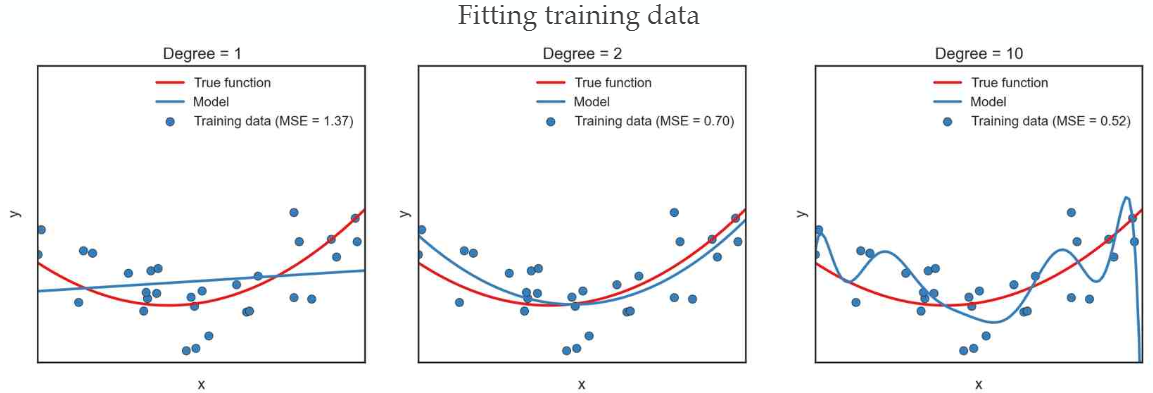
\includegraphics[scale=.3]{gfx/overfitting.png}
	\caption{Fen\'omeno de sobreajuste en polinomios de alto grado}
\end{figure}


Dicho esto, la brecha entre el riesgo emp\'irico y el riesgo esperado puede ser mayor para un conjunto de polinomios de alto grado ya que su alta capacidad les permite sobreajustar un conjunto dado de datos de entrenamiento. (Ver \ref{gfx: overfitting})

Matem\'aticamente, con la capacidad de medici\'on de la dimensi\'on VC, se puede establecer uno de los resultados m\'as importantes en Machine Learning


\begin{proposition}[Cota en la complejidad algoritmica de la estimaci\'on riesgo]
	Sea $d_{ \mathcal{H} }$ la dimensi\'on VC de $\mathcal{H}$ una familia de funciones generalizadora, luego se tiene una probabilidad de al menos $1 - \eta$ que:

\begin{equation}
\label{eq: Cota complejidad algoritmica para distancia de riesgos}
\sup\limits_{h \in \mathcal{H}} {\abs{R(h) - R_n(h)}} \leq \mathcal{O} \left( \sqrt{\frac{1}{2n} \log \left(\frac{2}{\eta}\right) + \frac{d_{\mathcal{H}}}{n} \log \left( \frac{n}{d_{\mathcal{H}}} \right) } \right)
\end{equation}

\end{proposition}

Este l\'imite proporciona una imagen m\'as precisa de la dependencia de la brecha en la elecci\'on de $\mathcal{H}$. Por ejemplo, muestra que para una $d_{ \mathcal{H} }$ fija, se obtiene una convergencia uniforme aumentando el n\'umero de puntos de entrenamiento $n$. Sin embargo, tambi\'en muestra que, para una $n$ fija, la brecha puede ensancharse si aumento $d_{ \mathcal{H} }$. De hecho, para mantener la misma brecha, se debe aumentar $n$ a la misma tasa si $d_{ \mathcal{H} }$ se incrementa. La convergencia uniforme incorporada en este resultado es crucial en el machine learning, ya que uno quiere asegurarse de que el sistema de predicci\'on funciona bien con cualquier dato que se le proporcione. 


Curiosamente, una cantidad que no ingresa en (\ref{eq: Cota complejidad algoritmica para distancia de riesgos}) es el n\'umero de par\'ametros que distinguen a una funci\'on miembro particular $h$ de la familia $\mathcal{H}$. En algunos entornos, como la regresi\'on log\'istica, este n\'umero es esencialmente el mismo que $d_{ \mathcal{H} }$, lo que podr\'ia sugerir que la tarea de optimizar sobre $h \in \mathcal{H} $ es m\'as engorrosa a medida que $d_{ \mathcal{H} }$ aumenta. Sin embargo, este no es siempre el caso. Ciertas familias de funciones son m\'as amenas para minimizar a pesar de tener un n\'umero muy grande o incluso infinito de par\'ametros; en \cite{vapnik:1998} se dise\~naron para aprovechar este hecho [Ver Teorema 10.3].

En general, mientras que los l\'imites tales como (\ref{eq: Cota complejidad algoritmica para distancia de riesgos}) son te\'oricamente interesantes y proporcionan una visi\'on \'util, raramente se usan directamente en la pr\'actica ya que generalmente es m\'as f\'acil estimar la brecha entre riesgo emp\'irico y riesgo esperado con experimentos de \textit{validaci\'on cruzada}. Ahora presentaremos ideas subyacentes a un marco pr\'actico que respeta las concesiones mencionadas anteriormente.

\subsection{Minimizaci\'on de riesgos estructurales}

Un enfoque para elegir una funci\'on de predicci\'on que ha demostrado ser ampliamente exitosa en la pr\'actica es la \textit{minimizaci\'on del riesgo estructural} \cite{vapnik:1974}, \cite{vapnik:1998}. En lugar de elegir una familia gen\'erica de funciones de predicci\'on, sobre las cuales ser\'ia dif\'icil optimizar y estimar la brecha entre los riesgos emp\'iricos y los esperados, se elige una \textit{estructura}, es decir, una colecci\'on de familias de funciones anidadas. Por ejemplo, dicha estructura se puede formar como una colecci\'on de subconjuntos de una determinada familia $\mathcal{H}$ de la siguiente manera: dada una funci\'on de preferencia $\Omega$, elegir varios valores de un \textit{hiperpar\'ametro} $C$, de acuerdo con cada uno de los cuales se obtiene el subconjunto $\mathcal{H}_C := \left\lbrace h \in \mathcal{H} : \Omega (h) \leq C \right\rbrace$. Dado un n\'umero fijo de ejemplos, el aumento de $C$ reduce el riesgo emp\'irico (es decir, el m\'inimo de $R_n (h) $ sobre $h \in \mathcal{H}_C$), pero, despu\'es de cierto punto, t\'ipicamente aumenta la brecha entre los riesgos esperado y emp\'irico. Este fen\'omeno se ilustra en la Figura \ref{gfx: hiperparametros}.


Otras formas de introducir estructuras son considerar un riesgo emp\'irico regularizado $R_n (h) + \lambda \Omega (h)$  que puede verse como el Lagrangiano para minimizar $R_n (h)$ sujeto a $\Omega (h) \leq C$).

\begin{figure}[h]
	\label{gfx: hiperparametros}
	\centering
	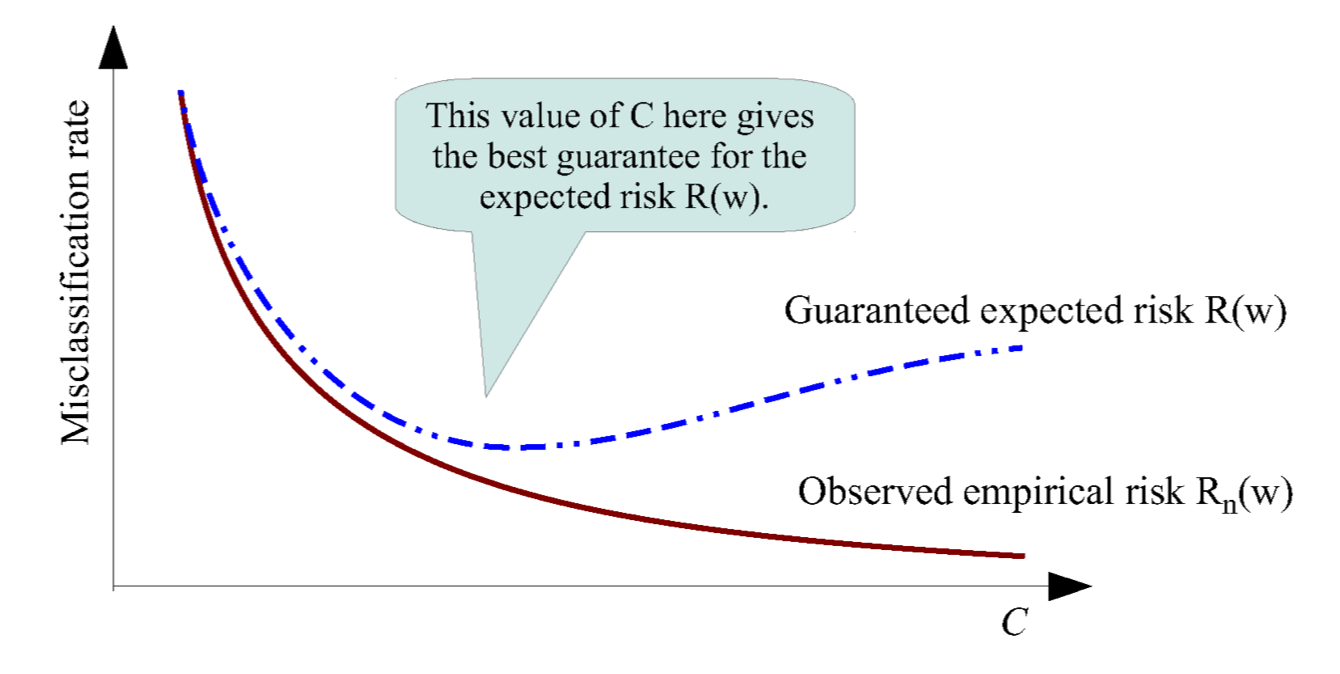
\includegraphics[scale=.3]{gfx/hyperparametros.png}
	\caption{Fen\'omeno de distancia de los riesgos en funcion de la evoluci\'on de hiperpar\'ametros}
\end{figure}

Dada tal configuraci\'on, uno puede evitar estimar la brecha entre el riesgo emp\'irico y esperado dividiendo los datos disponibles en subconjuntos: un \textit{conjunto de entrenamiento} utilizado para producir un subconjunto de soluciones candidatas, un \textit{conjunto de validaci\'on} utilizado para estimar el riesgo esperado para cada candidato, y un \textit{conjunto de prueba} utilizado para estimar el riesgo esperado para el candidato que finalmente se elige. Espec\'ificamente, sobre el conjunto de entrenamiento, uno minimiza una medida de riesgo emp\'irico $R_n$ sobre $\mathcal{H}_C$ para varios valores de $C$. Esto da como resultado un pu\~nado de funciones candidatas. El conjunto de validaci\'on se usa para estimar el riesgo esperado correspondiente a cada soluci\'on candidata, luego de lo cual se elige la funci\'on que arroje el menor valor de riesgo estimado. Suponiendo que se ha utilizado un rango suficientemente grande para $C$, a menudo se encuentra que la mejor soluci\'on no corresponde al mayor valor de $C$ considerado; nuevamente, vea la Figura \ref{gfx: hiperparametros}.


Otro camino, aunque indirecto, hacia la minimizaci\'on del riesgo es emplear un algoritmo para minimizar $R_n$, pero terminar el algoritmo \textit{antes} de que se encuentre un minimizador real de $R_n$. De esta manera, el papel del hiperpar\'ametro lo asume el tiempo de entrenamiento permitido, seg\'un el cual uno encuentra t\'ipicamente las relaciones ilustradas en la Figura \ref{gfx: stopping}. Los an\'alisis te\'oricos relacionados con la idea de la detenci\'on temprana son mucho m\'as desafiantes que los de otras formas de minimizaci\'on del riesgo estructural. Sin embargo, vale la pena mencionar estos efectos ya que la detenci\'on temprana es una t\'ecnica popular en la pr\'actica y, a menudo, es \textit{esencial} debido a las limitaciones del presupuesto computacional.


\begin{figure}[h]
	\label{gfx: stopping}
	\centering
	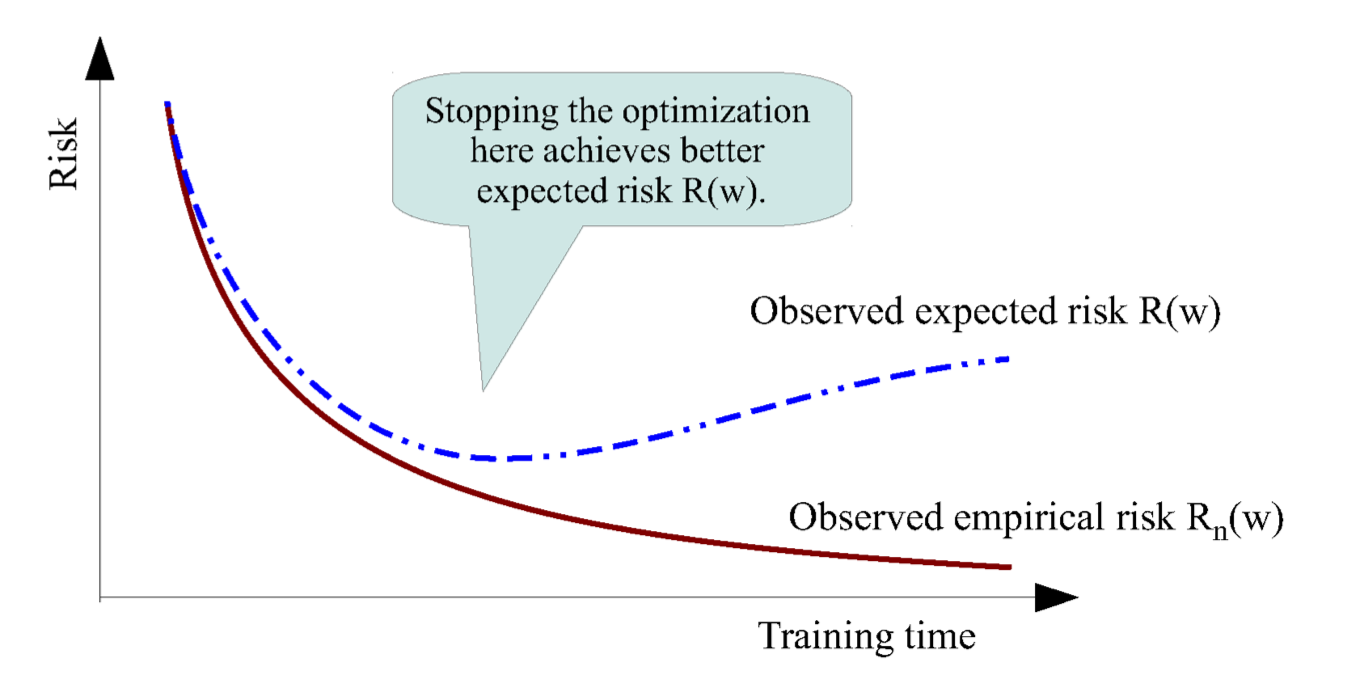
\includegraphics[scale=.3]{gfx/stopping.png}
	\caption{Ilustraci\'on de la detenci\'on temprana. Detener prematuramente la optimizaci\'on del riesgo emp\'irico $R_n$ a menudo resulta en un mejor riesgo esperado $R$. De esta manera, el tiempo de parada juega un papel similar al del hiperpar\'ametro C en la ilustraci\'on de minimizaci\'on de riesgo estructural}
\end{figure}


En general, el principio de minimizaci\'on del riesgo estructural ha demostrado ser \'util para muchas aplicaciones. En lugar de codificar el conocimiento como reglas formales de clasificaci\'on, uno lo codifica mediante preferencias para ciertas funciones de predicci\'on sobre otras, luego explora el rendimiento de varias funciones de predicci\'on que se han optimizado bajo la influencia de dichas preferencias.

\section{Enunciados de problemas de optimizaci\'on formal}

Los problemas de optimizaci\'on en el machine learning surgen a trav\'es de la definici\'on de las funciones de predicci\'on y p\'erdida que aparecen en las mediciones de riesgo esperado y emp\'irico que se pretenden minimizar. Nuestras discusiones giran en torno a las siguientes definiciones.

\subsection{Funciones de Predicci\'on y P\'erdida}
En lugar de considerar un problema de optimizaci\'on variacional sobre una familia gen\'erica de funciones de predicci\'on, suponemos que la funci\'on de predicci\'on $h$ tiene una forma fija y est\'a parametrizada por un vector real $w \in \mathbb{R}^d $ d sobre el cual se realizar\'a la optimizaci\'on. Formalmente, para algunos $h(\cdot ; \cdot): \mathbb{R}^{d_x} \times \mathbb{R}^d \rightarrow \mathbb{R}^{d_y}$ dados y, considerandos la familia de funciones de predicci\'on

\begin{equation}
\mathcal{H} := \lbrace h(\cdot ; w): w \in \mathbb{R}^d \rbrace
\end{equation}

Nuestro objetivo es encontrar la funci\'on de predicci\'on en esta familia que minimice las p\'erdidas incurridas por predicciones inexactas. Para este prop\'osito, asumimos una funci\'on de p\'erdida dada $ \ell : \mathbb{R}^{d_y} \times \mathbb{R}^{d_y} \rightarrow \mathbb{R}$ como aquella que, dado un par de entrada-salida $(x, y)$, produce la p\'erdida $ \ell (h(x;w),y)$ cuando $h (x; w)$ e $y$ son las salidas predichas y verdaderas, respectivamente.

\subsection{Riesgo esperado}
Idealmente, el vector de par\'ametros $\omega$ se elige para minimizar la p\'erdida esperada en la que se incurrir\'ia con \textit{cualquier} par de entrada-salida. Para expresar esta idea formalmente, suponemos que las p\'erdidas se miden con respecto a una distribuci\'on de probabilidad $P (x, y)$ que representa la verdadera relaci\'on entre las entradas y las salidas. Es decir, suponemos que el espacio de entrada-salida $\mathbb{R}^{d_x} \times \mathbb{R}^{d_y}$ est\'a dotado con $P: \mathbb{R}^{d_x} \times \mathbb{R}^{d_y} \rightarrow [0,1]$ y la funci\'on objetivo que deseamos minimizar es

\begin{equation}
\label{eq: Riesgo esperado}
R(w) = \int\limits_{\mathbb{R}^{d_x}\times \mathbb{R}^{d_y}} {\ell \left(h(x;w), y\right) dP(x,y)} = \mathbb{E} \left[ \ell \left( h(x;w), y \right) \right]
\end{equation}

Decimos que $R : \mathbb{R}^{d} \rightarrow \mathbb{R}$ produce el \textit{riesgo esperado} (es decir, la p\'erdida esperada) dado un vector de par\'ametro $w$ con una respectiva distribuci\'on de probabilidad $P$.

\subsection{Riesgo emp\'irico}
Si bien puede ser deseable minimizar (\ref{eq: Riesgo esperado}), tal objetivo es insostenible cuando no se cuenta con informaci\'on completa sobre $P$. Por lo tanto, en la pr\'actica, uno busca la soluci\'on de un problema que involucra una estimaci\'on del riesgo esperado $R$. En el aprendizaje supervisado, uno tiene acceso (ya sea de una vez o de manera incremental) a un conjunto de  $n \in \mathbb{N}$ muestras de entrada y salida independientes $\left\lbrace (x_i, y_i) \right\rbrace_{i=1}^{n} \subset \mathbb{R}^{d_x} \times \mathbb{R}^{d_y}$, con las cuales se puede definir la funci\'on de riesgo emp\'irico $R_n : \mathbb{R}^d \rightarrow \mathbb{R}$ dada por la ecuaci\'on 

\begin{equation}
\label{eq: Riesgo empirico}
R_n(\omega) = \frac{1}{n} \sum\limits_{i=1}^{n} {l \left( h(x;w), y\right)}
\end{equation}

En t\'erminos generales, la minimizaci\'on de $R_n$ puede considerarse el problema pr\'actico de optimizaci\'on de inter\'es. Por ahora, consideramos la medida no regularizada (\ref{eq: Riesgo empirico}), pero notemos que los m\'etodos de optimizaci\'on que discutiremos en las secciones siguientes pueden aplicarse f\'acilmente cuando se incluye un t\'ermino suave de regularizaci\'on.

\subsection{Notaci\'on simplificada}
Las expresiones (\ref{eq: Riesgo empirico}) y (\ref{eq: Riesgo esperado}) muestran expl\'icitamente c\'omo los riesgos esperado y emp\'irico dependen de la funci\'on de p\'erdida, espacio de muestra o conjunto de muestras, etc. Sin embargo, cuando hablamos de m\'etodos de optimizaci\'on, a menudo emplearemos una notaci\'on simplificada que tambi\'en ofrece algunos caminos para generalizar ciertas ideas algor\'itmicas. En particular, representemos una muestra (o conjunto de muestras) por una variable aleatoria $\upxi$; por ejemplo, uno puede imaginar una realizaci\'on de $\upxi$ como una muestra \'unica $(x, y)$ de $\mathbb{R}^{d_x} \times \mathbb{R}^{d_y}$, o una realizaci\'on de $\upxi$ podr\'ia ser un conjunto de muestras $\left\lbrace(x_i, y_i)\right\rbrace_{i \in S}$. Adem\'as, podemos referirnos a la p\'erdida incurrida para un dado $(w, \upxi)$ como $g (w; \upxi )$, es decir, $g$ es la composici\'on de la funci\'on de p\'erdida y la funci\'on de predicci\'on $h$.

De esta manera, el riesgo esperado para una $w$ dada es el valor esperado de esta funci\'on compuesta tomada con respecto a la distribuci\'on de $\upxi$:

\begin{equation}
\label{Riesgo esperado 3}
R(w) = \mathbb{E} \left [ g(w; \upxi) \right ]
\end{equation}

De manera similar, dado un conjunto de realizaciones $\left\lbrace \upxi_{\left [ i \right ]} \right\rbrace _{i=1}^{n}$ de $\upxi$ correspondientes a un conjunto de muestras $\left\lbrace (x_i, y_i) \right\rbrace_{i=1}^{n}$, definamos la p\'erdida incurrida por el vector de par\'ametro $w$ con respecto a la i-\'esima muestra como

\begin{equation}
\label{funci\'on p\'erdida de w}
g_i (w) := g(w, \upxi_{\left [ i \right ]})
\end{equation}

y luego escribamos el riesgo emp\'irico como el promedio de las p\'erdidas de la muestra:

\begin{equation}
\label{Riesgo empirico 3}
R_n(w) = \frac{1}{n}\sum\limits_{i=1}^{n} g_i (w)
\end{equation}

Para referencia futura, usamos $\upxi_{\left [ i \right ]}$ para denotar el i-\'esimo elemento de un conjunto fijo de realizaciones de una variable aleatoria $\upxi$, mientras que, comenzando en la parte \ref{pt:algoritmosestocasticos}, utilizaremos $\upxi_{\left [ k \right ]}$ para denotar el k-\'esimo elemento de una secuencia de variables aleatorias .

\subsection{M\'etodos Estoc\'asticos vs. Optimizaci\'on por Batch}
Ahora vamos a introducir algunos algoritmos de optimizaci\'on fundamentales para minimizar el riesgo. Por el momento, dado que es la configuraci\'on t\'ipica en la pr\'actica, presentamos dos clases de algoritmo en el contexto de minimizar el riesgo emp\'irico medido $R_n$ en (\ref{Riesgo empirico 3}). Hay que tener en cuenta, sin embargo, que gran parte de nuestra discusi\'on posterior se centrar\'a en el rendimiento de los algoritmos al considerar la verdadera medida de inter\'es, es decir, el riesgo esperado $R$ en (\ref{Riesgo esperado 3}).

Los m\'etodos de optimizaci\'on para el machine learning se dividen en dos grandes categor\'ias. Nos referimos a ellos como estoc\'asticos y por Batch. El m\'etodo protot\'ipico de optimizaci\'on estoc\'astica es el m\'etodo del gradiente estoc\'astico (DE) \cite{robbins:1951}, que, en el contexto de minimizar $R_n$ y con $w_1\in \mathbb{R}^d$ dado, se define por
\begin{equation}
\label{def: DE}
w_{k+1} \gets w_k - \alpha_k \nabla g_{i_k} (w_k)
\end{equation}

Aqu\'i, para todo $k \in \mathbb{N} := \left\lbrace 1, 2, ... \right\rbrace $, el \'indice $i_k$ (correspondiente a la variable aleatoria $\upxi_{\left[ i_k \right]}$, es decir, el par de muestras $(x_{i_k}, y_{i_k})$) se elige \textit{al azar} de $\left\lbrace 1,. . . , n \right\rbrace$ y $\alpha _k$ es un incremento positivo. Cada iteraci\'on de este m\'etodo es, por lo tanto, muy barata, y solo incluye el c\'alculo del gradiente $\nabla g_{i_k} (w_k)$ correspondiente a una muestra. El m\'etodo es notable porque la secuencia de iteraci\'on no est\'a determinada \'unicamente por el
	la funci\'on $R_n$, el punto de inicio $w_1$, y la secuencia de incrementos $\left\lbrace \alpha _k \right\rbrace $, como lo har\'ia en un algoritmo de optimizaci\'on determinista. Por el contrario, $\left\lbrace w_k \right\rbrace $ es un proceso estoc\'astico cuyo comportamiento est\'a determinado por la secuencia aleatoria $\left\lbrace i_k \right\rbrace $. A\'un as\'i, como veremos en nuestro an\'alisis en el cap\'itulo \ref{ch:convergenciaL1}, mientras que cada direcci\'on $- \nabla g_{i_k} (w_k)$ podr\'ia no ser una de descendencia de $w_k$ (en el sentido de producir una derivada direccional negativa para $R_n$ de $w_k$), s\'i es una direcci\'on de descenso \textit{en esperanza}, luego la secuencia $\left\lbrace w_k \right\rbrace $ puede guiarse hacia un minimizador de $R_n$.
	
	Para muchos en la comunidad de investigaci\'on de optimizaci\'on, un enfoque por \textit{Batch} es una idea m\'as natural y conocida. El m\'etodo m\'as simple de esta clase es el algoritmo de descenso m\'as pronunciado -tambi\'en conocido como gradiente, descenso de gradiente por Batch o m\'etodo de gradiente completo- (GD)que se define mediante la siguiente iteraci\'on:
	
	\begin{equation}
	\label{gradiente de Batch}
	w_{k+1} \gets w_k - \alpha_k \nabla R_n(w_k) = w_k -\frac{\alpha_k}{n} \sum\limits_{i=1}^{n} {\nabla g_i (w_k)}
	\end{equation}
	
	Calcular el paso $- \alpha_k \nabla R_n (w_k)$ en tal enfoque es m\'as costoso que calcular el paso $- \alpha_k \nabla g_{i_k} (w_k)$ en DE, aunque se puede esperar que se calcule un mejor paso cuando todas las muestras se consideran en una iteraci\'on.
	
	Los enfoques estoc\'astico y por Batch ofrecen diferentes compensaciones en t\'erminos de costos de iteraci\'on y mejora esperada de la iteraci\'on para minimizar el riesgo emp\'irico. ¿Por qu\'e, entonces, DE ha alcanzado tal prominencia en el contexto del machine learning a gran escala? Comprender el razonamiento detr\'as de esto requiere una consideraci\'on cuidadosa de las compensaciones computacionales entre los m\'etodos estoc\'astico y por Batch, as\'i como una mirada m\'as profunda en sus habilidades para garantizar la mejora en el subyacente riesgo esperado $R$. Comenzaremos a investigar estos temas en la siguiente subsecci\'on.
	
	\section{Motivaci\'on para los m\'etodos estoc\'asticos}
	Antes de analizar las fortalezas de los m\'etodos estoc\'asticos, como DE, no se debe perder de vista el hecho de que los enfoques por Batch poseen algunas ventajas intr\'insecas. Primero, cuando uno ha reducido el problema estoc\'astico de minimizar el riesgo esperado $R$ para enfocarse exclusivamente en el problema determinista de minimizar el riesgo emp\'irico $R_n$, el uso de informaci\'on de gradiente completo en cada iteraci\'on abre la puerta para muchos m\'etodos de optimizaci\'on determin\'isticos basados en gradiente. Es decir, en un enfoque por Batch, uno tiene a su disposici\'on la gran cantidad de t\'ecnicas de optimizaci\'on no lineal que se han desarrollado en las \'ultimas d\'ecadas, incluido el m\'etodo de gradiente completo o gradiente de Batch (\ref{gradiente de Batch}), pero tambi\'en gradiente acelerado, gradiente conjugado, cuasi-Newton y m\'etodos inexactos de Newton \cite{nocedal:2006}. Segundo, debido a la estructura de suma de $R_n$, un m\'etodo por Batch puede beneficiarse f\'acilmente de la paralelizaci\'on ya que la mayor parte del c\'alculo se basa en evaluaciones de $R_n$ y $\nabla R_n$. Los c\'alculos de estas cantidades pueden incluso realizarse de forma distribuida.
	
	A pesar de estas ventajas, existen razones intuitivas, pr\'acticas y te\'oricas para seguir un enfoque estoc\'astico. Perm\'itanos motivarlos contrastando la iteraci\'on DE caracter\'istica (\ref{def: DE}) con la iteraci\'on de gradiente de Batch completo (\ref{gradiente de Batch}).
	
	\subsection{Motivación intuitiva}
	
	En un nivel intuitivo, DE emplea información de manera más eficiente que un método por batch. Para ver esto, considere una situación en la cual un conjunto de entrenamiento, llámelo $S$, consta de diez copias de un conjunto de $S_{sub}$. Un minimizador de riesgo empírico para el conjunto mayor $S$ está claramente dado por un minimizador para el conjunto más pequeño $S_{sub}$, pero si se aplicara un enfoque por batch para minimizar $R_n$ sobre $S$, entonces cada iteración sería diez veces más costosa que si solo uno tenía una copia de $S_{sub}$. Por otro lado, DE realiza los mismos cálculos en ambos escenarios, en el sentido de que los cálculos de gradientes estocásticos implican la elección de elementos de $S_{sub}$ con las mismas probabilidades. En realidad, un conjunto de entrenamiento típicamente no consiste en duplicados exactos de datos de muestra, pero en muchas aplicaciones a gran escala los datos involucran una buena cantidad de redundancia (aproximada). Esto sugiere que usar todos los datos de muestra en cada iteración de optimización es ineficiente.
	
	Se puede llegar a una conclusión similar con el uso de conjuntos de entrenamiento, validación y prueba. Si uno cree que trabajar con solo, por ejemplo, la mitad de los datos en el conjunto de entrenamiento  es suficiente para hacer buenas predicciones sobre datos no vistos, entonces uno puede argumentar en contra de trabajar con todo el conjunto de entrenamiento en cada iteración de optimización. Repitiendo este argumento, trabajar con solo una cuarta parte del conjunto de entrenamiento puede ser útil al inicio, o incluso con solo un octavo de los datos, y así sucesivamente. De esta manera, llegamos a la motivación de la idea de que trabajar con muestras pequeñas, al menos inicialmente, puede ser bastante atractivo.
	
	\subsection{Motivación práctica}
	
	 Los beneficios intuitivos que acabamos de describir se han observado repetidamente en la práctica, donde a menudo se encuentran ventajas muy reales de SG en muchas aplicaciones. Como ejemplo, la Figura \ref{gfx: de} compara el rendimiento de un método \textbf{L-BFGS} por batch \cite{liu:1989} \cite{nocedal:1980} y el método DE \ref{def: DE} con un incremento constante (es decir, $\alpha_k = \alpha$ para todos $k \in \N$) en un problema de clasificación binario que utiliza una función objetivo de pérdida logística y los datos del conjunto de datos RCV1. La figura traza el riesgo empírico $R_n$ en función del número de accesos de una muestra del conjunto de entrenamiento, es decir, el número de evaluaciones de un gradiente de muestra $\nabla f_{i_k}(w_k)$. Cada conjunto de $n$ accesos consecutivos se llama \textit{epoch}. El método por batch solo realiza un paso por \textit{epoch}, mientras que DE realiza $n$ pasos por \textit{epoch}. La trama muestra el comportamiento en los primeros 10 \textit{epochs}. La ventaja de DE es llamativa y representativa del comportamiento típico en la práctica. (Sin embargo, se debe tener en cuenta que para obtener un comportamiento tan eficiente, era necesario ejecutar DE varias veces usando diferentes opciones para $\alpha$ hasta que se identificara una buena opción para este problema en particular. Discutimos cuestiones teóricas y prácticas relacionadas con la elección de incrementos en nuestro análisis en la parte \ref{pt:algoritmosestocasticos})


\begin{figure}[h]
	\label{gfx: de}
	\centering
	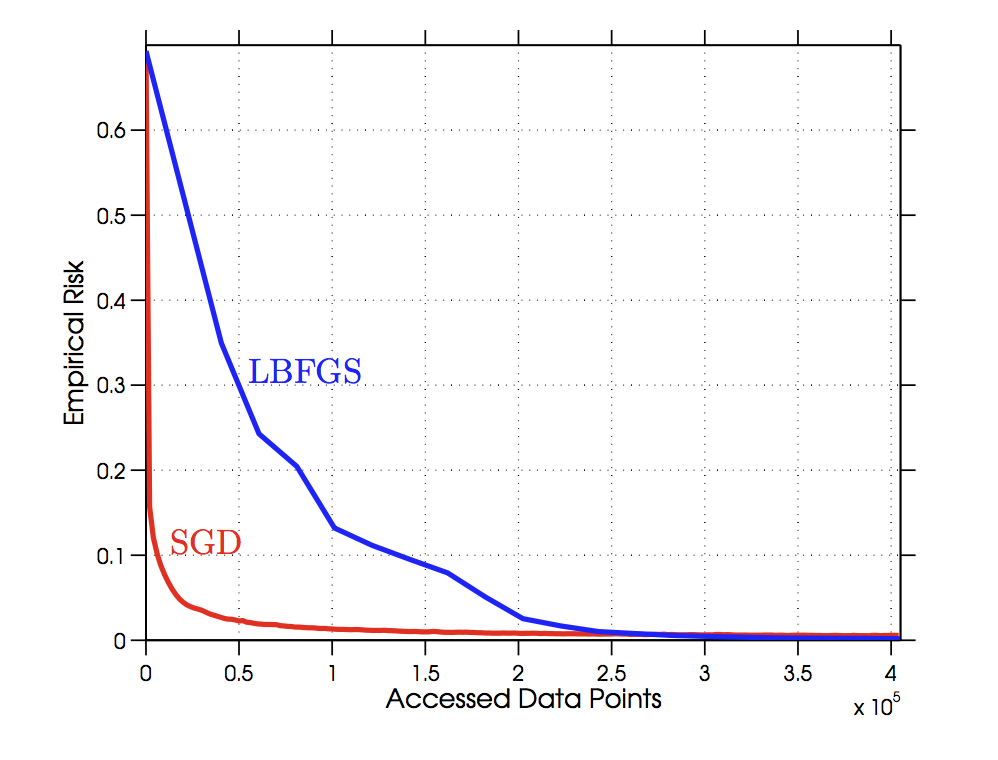
\includegraphics[scale=.3]{gfx/de.png}
	\caption{Riesgo empírico $R_n$ en función del número de puntos de datos accedidos (ADP) para un método \textbf{L-BFGS} por batch y el método de gradiente estocástico (DE) \ref{def: DE} en un problema de clasificación binaria con un objetivo de pérdida logística y el conjunto de datos RCV1. SG se ejecutó con un incremento fijo de $\alpha  = 4$}
\end{figure}

\subsection{Motivación Teórica }

También se pueden citar argumentos teóricos para una preferencia de DE sobre un enfoque por batch. Vamos a dar una vista previa de estos argumentos ahora, que se estudian con más profundidad y más detalles en la parte \ref{pt:algoritmosestocasticos}:

\begin{itemize}
	\item Es bien sabido que un enfoque por batch puede minimizar $R_n$ a un ritmo rápido; por ejemplo, si $R_n$ es fuertemente convexo (ver \ref{def: Fuertemente convexa}) y uno aplica un método de descenso de gradiente por batch, entonces existe una constante $\rho \in (0,1)$ tal que, para todo $k \in \N$, el error de entrenamiento satisface:
	
	\begin{equation}
		\label{Complejidad riesgo en batch}
		R_n(w_k) - R_n^* \leq \mathcal{O} \left(\rho^k\right)
	\end{equation}
	
	Donde $R_n^*$ denota el valor mínimo de $R_n$. La velocidad de convergencia exhibida aquí se conoce como \textit{convergencia lineal} en la bibliograf\'ia de optimización \cite{ortega:2000} y \textit{convergencia geométrica} en la comunidad de investigación de machine learning; simplemente nos referiremos a él como convergencia lineal. De \ref{Complejidad riesgo en batch}, se puede concluir que, en el peor de los casos, el número total de iteraciones en las que el error de entrenamiento puede estar por encima de un valor dado de $\epsilon >0$ es proporcional a $\log \left(\frac{1}{\epsilon}\right)$. Esto significa que, con un costo por iteración proporcional a $n$ (debido a la necesidad de calcular $\nabla R_n(w_k)$ para todo $k \in \N$), el trabajo total requerido para obtener $\epsilon-$optimalidad para un método de gradiente por batch es proporcional a $n \log\left(\frac{1}{\epsilon}\right)$.
	
	\item La velocidad de convergencia de un método estocástico básico es más lenta que para un método de gradiente por batch; por ejemplo, si $R_n$ es estrictamente convexo y cada $i_k$ se muestrea uniformemente desde en $\sett{1, \dots, n}$, entonces, para todo $k \in \N$, las iteraciones DE satisfacen la propiedad de convergencia sublineal (ver \ref{theorem: DE en fuertemente convexo y alfa decreciente converge en l1}):
	
	\begin{equation}
		\label{Complejidad riesgo en de}
		\expectation{R_n(w_k) - R_n^*} = \mathcal{O} \left(\frac{1}{k}\right)
	\end{equation}
	
	Sin embargo, es cr\'itico notar que ni el costo de iteración ni el orden dependen del tamaño del conjunto de muestras $n$. Esto significa que el trabajo total requerido para obtener $\epsilon-$optimalidad para DE es proporcional a $\frac{1}{\epsilon}$. Es cierto que esto puede ser mayor que $n \log \left(\frac{1}{\epsilon}\right)$ para valores chicos de $n, \epsilon$, pero la comparación favorece a DE cuando se pasa al régimen de \textit{big data} donde $n$ es grande y uno es simplemente limitado por un presupuesto de tiempo computacional.
	
	\item Otra característica importante de DE es que produce la misma velocidad de convergencia que en \ref{Complejidad riesgo en de} para el error en el riesgo esperado, $R - R^**$, donde $R^*$ es el valor mínimo de $R$. Específicamente, aplicando la iteración DE, pero con $g(wk, \upxi_{k})$ reemplazado por $\nabla f (w_k; \upxi_{k})$ con cada $\upxi_{k}$ tomado independientemente de acuerdo con la distribución P, vale:
	
	\begin{equation}
		\expectation{R(w_k) - R^*} = \mathcal{O} \left(\frac{1}{k}\right)
	\end{equation}
	
	Que nuevamente es una velocidad sublineal pero en el riesgo esperado, algo que es imposible estimar en los m\'etodos de batch. Por lo tanto, deducimos que en el regimen de \textit{big data} minimizar el riesgo emp\'irico o el riesgo esperado es equivalente, lo que potencia la generalidad de las soluciones halladas por DE.
	
\end{itemize}

En resumen, existen argumentos intuitivos, prácticos y teóricos a favor de enfoques estocásticos sobre por batches en métodos de optimización para el machine learning a gran escala. Sin embargo, no pretendemos que los métodos por batch no tengan lugar en la práctica, si la Figura \ref{gfx: stopping} uno considerara un mayor número de \textit{epochs}, entonces uno vería que el algoritmo de batch eventualmente mejora al método estocástico y produce un menor error de entrenamiento. Esto motiva por qué muchos métodos propuestos recientemente intentan combinar las mejores propiedades de los algoritmos por batch y estocásticos. Además, la iteración de DE es difícil de paralelizar y requiere una comunicación excesiva entre nodos en una configuración de computación distribuida, proporcionando un mayor impulso para el diseño de algoritmos de optimización nuevos y mejorados. \cite{agarwal:2017} \cite{atchade:2014}

\section{Organizaci\'on de la Tesis}

Esta Tesis esta organizada seg\'un la categorizaci\'on mas est\'andar de los algoritmos encontrados en Machine Learning.

La primer parte (\ref{pt:introduccion}) refiere a la motivaci\'on tanto matem\'atica como algoritmica y del \'area para analizar la convergencia de los algoritmos presentados, como a su vez los contenidos preliminares usados a lo largo del documento. Al final, en el cap\'itulo \ref{ch:resumen}, se incluye un resumen de los resultados vistos, pensando mayoritariamente  en el aplicante del Machine Learning que quiere r\'apidamente saber condiciones de convergencia para sus algoritmos.

La segunda parte (\ref{pt:algoritmosbatch}) trata exclusivamente los algoritmos deterministicos, comunmente denominados de \textit{tipo batch}. En el Cap\'itulo \ref{ch:convergenciaPuntual} , utilizando la gran referencia \cite{nesterov:2004}, analizamos la convergencia puntual del descenso de gradiente con condiciones de convexidad d\'ebil y luego la convergencia \textit{lineal} con convexidad mas fuerte. Luego en el cap\'itulo \ref{ch:teorema-de-variedad-estable} nos basamos en \cite{lee:2017} para ver a estos algoritmos como discretizaciones de sistemas din\'amicos y con elt eorema de la variedad estable conclu\'imos un m\'etodo pr\'actico para analizar la convergencia \textit{casi todo punto}; esta forma de analizar los algortitmos es aplicada en el cap\'itulo \ref{ch: aplicaciones} con varios algoritmos est\'andar en el \'area. Finalmente en el cap\'itulo \ref{ch:resultadosNegativos} nos basamos en \cite{du:2017} para ver que aunque se tiene convergencia \textit{casi todo punto}, la complijdad algoritmica del descenso de gradiente es exponencial.

Esto nos motiva pasar a analizar los algoritmos estoc\'asticos en la parte \ref{pt:algoritmosestocasticos}, donde nos basamos en \cite{bottou:1999} y \cite{bottou:2016} para analizar en el cap\'itulo \ref{ch:convergenciaL1} la convergencia en \textit{norma $L1$} al m\'inimo (o a un entorno de \'este) y finalmente en el cap\'itulo \ref{ch:convergenciaCTP} la convergencia \textit{casi todo punto} tanto en los casos convexo como no convexo, ya que el algoritmo induce un proceso estoc\'astico que induce una \textit{cuasi-martingala} convergente.

\smallskip

\chapter{Preliminares}\label{ch:preliminares}

\epigraph{Mathematics is the most beautiful and most powerful creation of the human spirit}{Stefan Banach}

\section{Espectro}

\begin{definition}
	Sea $f : X \rightarrow Y$, con $X,Y$ Banach, $f \in L(X,Y)$; definimos el espectro de $f$ de la siguiente manera:
	
	\begin{equation*}
		\sigma(f) = \sett{\alpha \in \C \tq f- \alpha \text{ no es inversible}}
	\end{equation*}
	
	Al supremo del espectro le decimos radio espectral (\eg $\rho(f) = \sup \sett{\abs{\alpha} \tq \alpha \in \sigma(f) }$)
	
\end{definition}

\begin{proposition}
	\label{prop: teorema de gelfand}
	Sea $f \in L(X,Y)$ un operador lineal acotado, entonces:
	
	\begin{equation*}
		\rho(f) = \lim \norm{f^n}^{\frac{1}{n}}
	\end{equation*}
	
\end{proposition}

\begin{proposition}
	\label{prop: calculo funcional}
	
	Sea $f \in L(X,Y)$ un operador lineal acotado y $h \in \mathcal{H}ol (U)$ con $\sigma(f) \subset U$ una funci\'on holomorfa en un entorno del espectro, entonces:
	
	\begin{equation*}
		\sigma \left(h(f)\right) = h(\sigma(f))
	\end{equation*}
	
\end{proposition}

\section{Variedades diferenciables y Teorema de la variedad estable}

Cuando estudiemos los algoritmos de tipo batch es normal analizar al algoritmo como $x_{k+1} \gets g(x_k)$ para una $g : X \rightarrow X$ inducida; o sea uno analiza las \'orbitas bajo la acci\'on de $g$ en una variedad dada $X$. Con esa motivaci\'on repasemos los conceptos b\'asicos de sistemas din\'amicos.

\subsection{Un repaso por Variedades}

\begin{definition}{[Cap\'itulo 1 de \cite{lee:00}]}
	Dado un espacio topol\'ogico $X$ decimos que es una variedad diferenciable de dimensi\'on $d$ si:
	
	\begin{itemize}
		\item $X$ es Haussdorf
		\item $X$ es $2-$contable
		\item Existe un atlas suave para $X$, o sea existe un conjunto de pares $\sett{\left(U_i, \phi_i\right)}$ tales que:
		
		\begin{enumerate}
			\item Para todo $x \in X$ existe $(U,\phi)$ con $x \in U$ y $\phi: U \rightarrow \phi{U}$ homeomorfismo
			\item Si existen dos cartas $(U,\phi), (V,\psi)$ en el entorno de $x$ con $U \cap V \neq \emptyset$ entonces $\phi \circ \psi^{-1} : \psi(U\cap V )\rightarrow \phi(U\cap V)$ es difeomorfismo
		\end{enumerate}
	\end{itemize}
	
\end{definition}

\begin{definition}{[Cap\'itulo 6 de \cite{lee:00}]}
	Dada una variedad de dimensi\'on $d \ \mani$ y el espacio de medida $\left(\R^d, \mathcal{B}, \mu\right)$, decimos que $E \subset \mani$ tiene \textit{medida cero} si existe un atlas $\mathcal{A} = \sett{U_i, \phi^i}_{i \in \N}$ tal que $\mu \left(\phi^i \left(E \cap U_i \right) \right) = 0$. En este caso usamos el abuso de notaci\'on $\mu(E) = 0$.
\end{definition}

\begin{definition}{[Cap\'itulo 3 de \cite{lee:00}]}
	El diferencial de $g$ es un operador lineal $D_g(x): \mathcal{T}_x \mapsto \mathcal{T}_{g (x)}$, donde $\mathcal{T}_x$ es el espacio tangente de $X$ en el punto $x$. Dada una curva $\gamma$
	en $X$ con $\gamma(0) = x$ y $d\gamma(0) = v \in \mathcal{T}_x$, el operador lineal se define como $D_g(x)v = \dfrac{d (g\circ \gamma)}{dt}(0) \in T_{g (x)}.$ El determinante del operador lineal $det (D_g (x))$ es el determinante de la matriz que representa $D_g (x)$ con respecto a una base arbitraria.
\end{definition}

\begin{proposition}
	Sea $X$ una variedad de dimensi\'on $d$, luego para todo $x \in X$ vale que $\mathcal{T}_x$ es un espacio vectorial de dimensi\'on $d$.
\end{proposition}

\begin{theorem}
	\label{theorem: Teorema de la funcion inversa}
	Sea $F: X \mapsto N$ una funci\'on diferenciable tal que $dF_x$ es un isomorfismo lineal, luego existe $x \in U \subset X$ abierto tal que $F \vert_U$ es un difeomorfismo  \eg $F, F^{-1} \in C^{\infty}(U)$
\end{theorem}

\begin{proposition}
	\label{prop: Localmente Lipshitz preserva medida}
	Sea $f : \R^d \rightarrow \R^d$ una funcion localmente Lipshitz, luego si $\mu(E) = 0$ vale que $\mu(f(E)) = 0$
\end{proposition}

\begin{lemma}
	\label{Difeomorfismos locales preservan medida cero}
	Sea $E \subset \mani$ tal que $\mu(E) = 0$; si $\det \left(Dg(x)\right) \neq 0$ para todo $x \in \mani$, luego $\mu\left(g^{-1}(E)\right) = 0$
\end{lemma}

\begin{proof}
	Sea $h = g^{-1}$ y $\left(V_i, \psi^i\right)$ una colecci\'on de cartas en el dominio de $g$, si verificamos que $\mu\left(h\left(E\right) \cap V_i\right) = 0$ para todo $i \in \N$ entonces:
	
	\begin{equation*}
	\mu(h(E)) = \mu \left(\Bigcup{i \in \N}{h(E) \cap V_i}\right) \le \Bigsum{i \in \N} \mu \left(h(E) \cap V_i\right) = 0
	\end{equation*}
	
	Sin p\'erdida de generalidad podemos asumir que $h(E) \subseteq V$ con $(V, \psi) \in \sett{(V_i, \phi^i)}$ una carta determinada. Sea $\mathcal{A} := \sett{\left(U_i, \varphi^i \right)}$ un atlas de $\mani$ y notemos $E_i = E \cap U_i$; luego $E = \Bigcup{i \in \N}{E_i} = \Bigcup{i \in \N}{{\varphi^i}^{-1} \circ \varphi^{i} \left(E_i\right)}$ por lo que:
	
	\begin{equation*}
	\begin{aligned}
	\mu\left(\psi \circ h(E)\right) & = & \mu \left(\psi \circ h \left(\Bigcup{i \in \N}{{\varphi^i}^{-1} \circ \varphi^{i} \left(E_i\right)}\right)\right)\\
	& \le & \Bigsum{i \in \N}{\mu \left(\psi \circ h \circ {\varphi^{i}}^{-1} \left(\varphi^i (E_i)\right)\right)}
	\end{aligned}
	\end{equation*}
	
	Por hip\'otesis $\varphi^i(E_i)$ es de medida cero, luego como $g$ es difeomorfismo local por \ref{theorem: Teorema de la funcion inversa}  entonces $\psi \circ h \circ {\varphi^{i}}^{-1} \in C^1$. Como si $f \in C^1(\R^d)$ entonces es localmente Lipshitz conclu\'imos por \ref{prop: Localmente Lipshitz preserva medida} que ${\mu \left(\psi \circ h \circ {\varphi^{i}}^{-1} \left(\varphi^i (E_i)\right)\right)} = 0$ para todo $i \in \N$. \qed
	
\end{proof}

Conclu\'imos con un resultado natural, pero no por eso menos crucial a la hora de ver la probabilidad de un conjunto dado en $X$.

\begin{proposition}
	\label{prop: Dimension menor tiene medida 0}
	Sea $N \inc M$ una subvariedad de dimensi\'on $n < m$, luego para todo $U \subset N$ abierto relativo vale que $\mu(U) = 0$
\end{proposition}

\subsection{Teorema de la variedad estable}

\begin{definition}
	Sea $f : \R^d \rightarrow \R$ tal que $f \in C^2$, luego:
	
	\begin{itemize}
		\item Un punto $x^*$ es cr\'itico de $f$  si $\nabla f(x^*) = 0$
		\item Un m\'inimo local si $x^*$ es cr\'itico y $\lambda_{min} \left(\nabla ^2 f(x^*)\right) > 0$
		\item Un punto silla estricto de $f$ si es cr\'itico y $\lambda_{min} \left(\nabla ^2 f(x^*)\right) < 0$ 
	\end{itemize}
	
	Notaremos $\mani^*$ al conjunto de puntos silla estrictos de $f$.
	
\end{definition}

\begin{theorem}
	\label{teo: variedad local estable central}
	Sea $x^*$ un punto fijo de $g \in C^{r}(\mani)$ un difeomorfismo local. Supongamos que $E = E_s \oplus E_u$ donde 
	
	\begin{equation*}
	\begin{aligned}
	E_s & = & \langle \sett{v_i \ / \ Dg(x^*)v_i = \lambda_i v_i \quad , \quad \lambda_i \le 1} \rangle \\
	E_u & = & \langle \sett{v_i \ / \ Dg(x^*)v_i = \lambda_i v_i \quad , \quad \lambda_i > 1} \rangle \\
	\end{aligned}
	\end{equation*}
	Entonces existe $W_{loc}^{cs} \inc \mani$ un \textit{embedding} $C^r$ local tangente a $E_s$ en $x^*$ llamado la \textit{variedad local estable central} que cumple que existe $B \ni x^*$ entorno tal que $g\left(W_{loc}^{cs}\right) \cap B \subseteq W_{loc}^{cs}$ y $\Bigcap{k \in \N}{g^{-k}(B)} \subseteq W_{loc}^{cs}$
\end{theorem}

\begin{proof}
	Ver Teorema III.1 de \cite{schub:1987}
\end{proof}

\section{Preliminares de Procesos Estoc\'asticos}

Debido a la naturaleza de los algoritmos estoc\'asticos, tiene sentido repasar los conceptos b\'asicos que utilizaremos en el estudio de ellos.

\subsection{Esperanza condicional}

Dado un espacio de probabilidad $\left(\Omega, \mathcal{F}, P\right)$ definimos una \textit{variable aleatoria } como una funci\'on $X : \Omega \mapsto \R$ tal que $X^{-1}(B) \in \mathcal{F}$ para todo $\B \in \mathcal{B}$ boreliano.

Por otro lado, dado un conjunto $\Omega$ y una familia $\left(X_{\gamma}\right)_{\gamma \in C}$ tal que $X_{\gamma}: \Omega \mapsto \R$ definimos la \textit{sigma algebra generada por las $X_\gamma$} $\mathcal{F} = \sigma\left(\sett{X_{\gamma}}\right)$ como la menor sigma \'algebra (en el sentido de la inclusi\'on) tal que todas las $X_{\gamma}$ son $\mathcal{F}$ medibles.

Recordemos adem\'as:

\begin{theorem}[Teorema de la convergencia mon\'otona]
	\label{theorem: Convergencia monotona}
	Sea $(f_n)$ una sucesi\'on positiva de elementos medibles en $(\Omega, \Sigma, \mu)$ un espacio de medida tal que $f_n \nearrow f$; luego:
	
	\begin{equation*}
		\int\limits_{\Omega} {f_n d\mu} \nearrow \int\limits_{\Omega}{f d\mu} 
	\end{equation*} 
\end{theorem}

\begin{theorem}[Teorema de la convergencia dominada]
	\label{theorem: Convergencia dominada}
	Sea $(f_n)$ una sucesi\'on de elementos medibles en $(\Omega, \Sigma, \mu)$ un espacio de medida tal que $f_n \nearrow f$ ctp; si existe $g \in L^1$ tal que $\abs{f_n} \leq g$ entonces:
	
	\begin{equation*}
	\int\limits_{\Omega} {\abs{f_n -f}d\mu} \rightarrow 0
	\end{equation*} 
\end{theorem}

\begin{remark}
	Una observaci\'on clave en el an\'alisis de los algoritmos de tipo estoc\'astico es que si llamamos ${W} := \sett{w_k}$ a las iteraciones del algoritmo, entonces notemos que podemos ver a $w_k$ como una variable aleatoria. En efecto, $w_k := w_{k-1} - \alpha_k g(w_k, .) : \Omega \rightarrow \R$ y por hip\'otesis es $\F$ medible; es m\'as, podemos ver a $W$ como un proceso estoc\'astico discreto.
\end{remark}

\begin{proposition}
	\label{def: esperanza condicional}
	Sea $\left(\Omega, \F, P\right)$ un espacio de probabilidad y $X$ una variable aleatoria tal que $X \in L^1(\Omega)$ ( \Eg $\expectation{\abs{X}} < \infty$). Si $\mathcal{G}$ es una sub-$\sigma-$algebra de $\F$ entonces existe $Y$ una variable aleatoria tal que:
	
	\begin{enumerate}
		\item $Y$ es $\mathcal{G}$ medible
		\item $Y \in L^1(\Omega)$
		\item Para todo $G \in \mathcal{G}$ vale:
		
		\begin{equation*}
			\int\limits_{G} {Y dP} = \int\limits_{G} {X dP}
		\end{equation*}
	\end{enumerate}

	Es m\'as, si $\widetilde{Y}$ es otra variable aleatoria que cumple las propiedades, entonces $Y = \widetilde{Y}$ ctp.
	
\end{proposition}

\begin{definition}
	Dados $X,\mathcal{G}$ como en la proposici\'on, a la variable aleatoria cuya existencia se prueba en \ref{def: esperanza condicional} se le llama \textit{una versi\'on de la esperanza condicional de $X$ dado $\mathcal{G}$} y se lo nota $\expectation{X \vert \mathcal{G}}$.
	
	A su vez, dada $Z$ ptra variable aleatoria definimos la \textit{esperanza condicional de $X$ dado $Z$} como $\expectation{X \vert Z} := \expectation{X \vert \sigma(Z)}$
	
\end{definition}

\begin{proof}
	Demostremos la existencia y unicidad:
	
	\begin{enumerate}
		\item {\textbf{Unicidad ctp}}
		
		Sea $X \in L^1$ e $Y,\widetilde{Y}$ dos versiones de $\expectation{X \vert \mathcal{G}}$ tal que no son iguales ctp, luego como $\sett{Y - \widetilde{Y} > \frac{1}{n}} \nearrow \sett{Y > \widetilde{Y}}$ existe $N$ tal que:
		
		\begin{equation*}
			P\left(Y - \widetilde{Y} > \frac{1}{N}\right) > 0
		\end{equation*}
		
		Luego como $Y, \widetilde{Y}$ son $\mathcal{G}$ medibles $\sett{Y - \widetilde{Y} > \frac{1}{N}} \in \mathcal{G}$ y entonces:
		
		\begin{equation*}
			0 \underbrace{=}_{Y,\widetilde{Y} = \expectation{X \vert \mathcal{G}}} \int\limits_{\sett{Y - \widetilde{Y} > \frac{1}{N}}} {Y - \widetilde{Y}} \geq \frac{1}{N} P \left(\sett{Y - \widetilde{Y} > \frac{1}{N}}\right) > 0
		\end{equation*}
		
		Luego $Y = \widetilde{Y}$ ctp.
		
		\item {\textbf{Existencia en $L^2$}}
		
		Sea $\mathcal{K} = L^2(\Omega, \mathcal{G}, P)$, sabemos que $\mathcal{K} $ es completo en $L^2$ y como $L^2$ es Hilbert existe $Y \in \mathcal{K} $ tal que:
		
		\begin{equation*}
			\expectation{\left(X - Y \right)^2} = \inf \sett{\expectation{\left(X - W \right)^2} \tq W \in \mathcal{K}}
		\end{equation*}
		
		\begin{equation*}
			\ip{X-Y, Z} = 0 \quad Z \in \mathcal{K}
		\end{equation*}
		
		Luego si $G \in \mathcal{G}$ entonces $Z = 1_{G} \in \mathcal{G}$ por lo que:
		
		\begin{equation*}
			\ip{X-Y, 1_G} = 0 \Longrightarrow \ \int\limits_{G} {XdP} = \int\limits_{G}{Y dP}
		\end{equation*}
		
		Conclu\'imos que $Y = \expectation{X \vert \mathcal{G}}$
		
		\item {\textbf{Existencia en $L^1$}}		
		
		Notemos que basta verlo para $X \geq 0$, luego existen $X_n \geq 0$ acotadas tal que $X_n \nearrow X$; como cada $X_n \in L^2$ si definimos $Y = \limsup \expectation{X_n \vert \mathcal{G}}$ entonces \ref{theorem: Convergencia monotona} demuestra lo que necesitabamos.\qed
		
	\end{enumerate}
	
\end{proof}

\begin{theorem}[Propiedades de la esperanza condicional]
	\label{theorem: Propiedades de esperanza condicional}
	Sea $\left(\Omega, \mathcal{F}, P\right)$ un espacio de medida, $X \in L^1$ y $\mathcal{G}, \mathcal{H}$ sub-$\sigma-$\'algebras de $\F$, luego:
	
	\begin{enumerate}
		\item $\expectation{\expectation{X \vert \mathcal{G}}} = \expectation{X}$
		\item Si $X$ es $\mathcal{G}$ medible entonces $X = \conditionalExpectation{X}{\G} $ ctp
		\item $\conditionalExpectation{aX + bY}{\G} = a\conditionalExpectation{X}{\G} + b \conditionalExpectation{Y}{\G}$
		\item Si $X \geq 0$ ctp, entonces $\conditionalExpectation{X}{\G} \geq 0$ ctp
		\item Si $0 \leq X_n \nearrow X$ entonces $\conditionalExpectation{X_n}{\G} \nearrow \conditionalExpectation{X}{\G}$
		\item Si $0 \leq X_n$ ctp entonces $\conditionalExpectation{\liminf X_n}{\G} \leq \liminf \conditionalExpectation{X_n}{\G}$
		\item Si $\abs{X_n} \leq V$ con $V \in L^1$ entonces si $X_n \rightarrow X$ ctp vale que $\conditionalExpectation{X_n}{\G} \rightarrow \conditionalExpectation{X}{G}$ ctp.
		\item Si $\mathcal{H}$ es una sub-$\sigma-$\'algebra de $\G$ entonces:
		
		\begin{equation*}
			\conditionalExpectation{X}{\G \vert \mathcal{H}} := \conditionalExpectation{\conditionalExpectation{X}{\G}}{\mathcal{H}} = \conditionalExpectation{X}{\mathcal{H}}
		\end{equation*}
		
		\item Si $Z$ es $\G$ medible y acotada entonces $\conditionalExpectation{ZX}{\G} = Z \conditionalExpectation{X}{\G}$ ctp
		\item Si $\mathcal{H}$ es independiente de $\sigma\left(\sigma(X), \G\right)$ entonces:
		
		\begin{equation*}
			\conditionalExpectation{X}{\sigma \left(\G, \mathcal{H}\right)} = \conditionalExpectation{X}{G} \ ctp
		\end{equation*}
		
		En particular, si $X$ es independiente de $\G$ vale que $\conditionalExpectation{X}{\G} = \expectation{X}$ ctp. 
		
	\end{enumerate}
	
\end{theorem}

\begin{proof}
	En general con cuentas bastante similares a las vistas en cualquier curso de An\'alisis Real teniendo cuidado de las proyecciones. Para una mejor referencia ver \cite{williams:1991}.
\end{proof}

\subsection{Martingalas y Cuasi-martingalas}

\begin{definition}
	Dada una sucesi\'on creciente (en el sentido de la inclusi\'on) de $\sigma$ \'algebras $\F_n \subset \F$ decimos que $\sett{\F_n}$ es una \textit{filtraci\'on} y que el espacio $\left(\Omega, \F, \sett{F_n}, P\right)$ es un espacio filtrado.
	
	Un proceso $X  = \left(X_n\right)$ decimos que es adaptado si $X_n $ es $\F_n$ medible para todo $n$ en un espacio filtrado.
	
	A su vez, dado un proceso $\left(X_n\right)$, \'este induce una filtraci\'on (llamada natural) en un espacio de probabilidad $\left(\Omega, \F, P\right)$ dada por $\F_n = \sigma\left(X_1, \dots, X_n \right)$
	
\end{definition}

\begin{definition}
	Dado un espacio filtrado, decimos que un proceso $X = \left(X_n\right)$ es una martingala relativa a la filtraci\'on $\sett{\F_n}$ si:
	
	\begin{itemize}
		\item $X$ es adaptado
		\item $X_n \in L^1$
		\item $\conditionalExpectation{X_n}{\F_{n-1}} = X_{n-1}$ ctp
	\end{itemize}

	A su vez decimos que es una (sub)supermartingala si vale la condici\'on $\conditionalExpectation{X_n}{\F_{n-1}} (\leq)\geq X_{n-1}$
	
\end{definition}

\begin{definition}
	Dado un espacio filtrado y $X$ un proceso integrable y adaptado, decimos que es una \textit{cuasi-martingala} si para todo $n \in \N$:
	
	\begin{equation}
		\mathbb{Var}_n(X) = \sup\limits_{J \subset \sett{1, \dots, n}} \sett{\expectation{\sum\limits_{\substack{i_k \in J \\ 1 \leq k \leq \abs{J}}}{\abs{\conditionalExpectation{X_{i_{k+1}} - X_{i_k}}{\F_{i_{k}}}}}}} < \infty
	\end{equation}
	
\end{definition}

\begin{remark}
	El concepto de cuasi-martingalas es una generalizaci\'on natural de las martingalas, submartingalas y supermartingalas. Fueron introducidos por primera vez por Fisk \cite{fisk:1965} para extender la descomposici\'on de Doob-Meyer a una clase m\'as grande de procesos. La forma en que las cuasimartingalas se relacionan con sub y s\'uper martingalas es muy similar a c\'omo las funciones de variaci\'on finita se relacionan con funciones crecientes y decrecientes. En particular, mediante la descomposici\'on de Jordan, cualquier funci\'on de variaci\'on finita en un intervalo se descompone como la suma de una funci\'on creciente y una funci\'on decreciente. De manera similar, un proceso estoc\'astico es una cuasimartingala si y solo si puede escribirse como la suma de una submartingala y una supermartingala. Este importante resultado fue mostrado primero por Rao \cite{rao:1969}, y signific\'o el inicio de la extensi\'on de gran parte de la teor\'ia de submartingalas  a cuasimartingalas.
\end{remark}

\begin{proposition}
	Toda martingala, submartingala o supermartingala es una cuasi-martingala
\end{proposition}

\begin{proof}
	En efecto, reemplazando $X$ por $-X$ podemos suponer que $\conditionalExpectation{X_{i_{k+1}} - X_{i_k}}{\F_{i_k}} \geq 0$, luego por \ref{theorem: Propiedades de esperanza condicional} resulta que $\mathbb{Var}_n(X) = \abs{\expectation{X_n - X_0}} < \infty$. \qed
\end{proof}

Ahora estamos en condiciones de enunciar el resultado principal de esta secci\'on: \textbf{El teorema de convergencia de cuasi-martingalas}. Este resultado es crucial en el an\'alisis de convergencia de algoritmos estoc\'asticos porque veremos m\'as adelante que el proceso estoc\'astico $\sett{w_k}$ inducido por el algoritmo induce una cuasi-martingala $\sett{w_k'}$ que ser\'a convergente; de lo cual deduciremos la convergencia de $\sett{w_k}$.

\begin{definition}
	\label{def: Variaciones positivas de un proceso}
	Dado un proceso estoc\'astico $\sett{u_k}$ adaptado a un espacio filtrado $\left(\Omega, \F, \sett{\mathcal{P}_k}, P\right)$ definimos el \textit{proceso de variaciones positivas} asociadas a $\sett{u_k}$ como :
	
	\begin{equation}
	\delta^u_k := \left\lbrace \begin{array}{cc}
	1 & \text{ si } \expectationfilt{u_{k+1} - u_k} > 0 \\
	0 & \text{ si no }
	\end{array}\right.
	\end{equation}
	
\end{definition}

\begin{theorem}[Teorema de convergencia de cuasi-martingalas]
	\label{theorem: Convergencia de cuasi martingalas}
	Dado un proceso estoc\'astico $\sett{u_k}$ adaptado a un espacio filtrado $\left(\Omega, \F, \sett{\mathcal{P}_k}, P\right)$ tal que:
	
	\begin{itemize}
		\item $u_k \geq 0$ ctp
		\item $\sum\limits_{k=1}^{\infty} {\expectation{\delta^u_k\left(u_{k+1} - u_k\right)}} < \infty$
	\end{itemize}
	
	Entonces $\sett{u_k}$ es una cuasi-martingala tal que $u_k \rightarrow u_{\infty} \geq 0$ ctp.
	
\end{theorem}

\begin{proof}
	Una buena revisi\'on de la demostraci\'on se encuentra en el cap\'itulo 9 de \cite{metivier:1983}
\end{proof}

\cleardoublepage
\setpartpreamble[u][\textwidth]{\vspace*{1cm} En esta parte vamos a analizar los tipos de convergencia de los diferentes algoritmos de primer orden de tipo batch usados en Machine Learning. A su vez vamos a analizar casos donde aunque la convergencia este, no es \'util computacionalmente}
\part{Algoritmos de tipo Batch}\label{pt:algoritmosbatch}
\chapter{Convergencia Puntual }\label{ch:convergenciaPuntual}

\epigraph{“El libro de la naturaleza esta escrito en el lenguaje de las Matem\'aticas"}{Galileo}

Si existe un algoritmo que todo estudiante o practicante del Machine Learning conoce, es el descenso de gradiente cl\'asico (o \textit{Descenso de gradiente en batch}) [Ver algoritmo \ref{algo: GD - intro}].

Un buen inicio es analizar la convergencia puntual del descenso de gradiente y bajo qu\'e condiciones se da. Para esto recordemos que dado una funci\'on de p\'erdida objetivo uno estima el \textit{riesgo esperado} por el \textit{riesgo emp\'irico} (Ver \ref{eq: Riesgo empirico}), luego considerando esto el algoritmo a analizar resulta:

\RestyleAlgo{boxruled}
\LinesNumbered
\begin{algorithm}[H]
	\caption{Descenso de gradiente en batch \label{algo: GD}}
	\textbf{Input:} $F: \R^d \rightarrow \R$, $f:\R^d \rightarrow \R$ tal que $f \in C^1$, $\alpha_k >0$, $N \in \N$, $w_1 \in \R^d$, $X = \sett{\upxi_j}_{j \leq N}$ \text{ muestra aleatoria i.i.d.} \\
	\For{$k \in \N$}{
		$w_{k+1} \gets w_{k} - \alpha_k \sum\limits_{j=1}^{N} \nabla F(\upxi_j) = w_{k} - \alpha_k \nabla R_N(w_k)$
	}
\end{algorithm}

Asumamos por esta secci\'on la siguiente condici\'on, que llamaremos \textit{convexidad d\'ebil}:

\begin{definition}
	\label{def: Debilmente convexo}
	Decimos que $F: \R^d \rightarrow \R$, $f:\R^d \rightarrow \R$ tal que $f \in C^1$ es \textit{d\'ebilmente convexo} si cumple las siguientes dos propiedades:
	
	\begin{itemize}
		\item Existe un \'unico $w^*$ tal que $F_{inf} := F(w^*) \leq F(w)$ para todo $w \in \R^n$.
		\item Para todo $\epsilon > 0$ vale que $\inf\limits_{\norm{w-w^*}^2 > \epsilon} {\left(w - w^*\right) \nabla F(w) > 0}$
	\end{itemize}
	
\end{definition}

\begin{remark}
	Si  $F: \R^d \rightarrow \R$, tal que $F \in C^1$ es convexa, entonces es d\'ebilmente convexa.
	
	En efecto, como $F$ es convexa existe $w* \in \R^d$ m\'inimo global y como $F \in C^1$ entonces $\nabla F(w^*) = 0$. Entonces $F$ cumple:
	
	\begin{equation*}
		\left(\nabla F(x) - \nabla F(y)\right)^T \left(x-y\right) >0
	\end{equation*}
	
	Para todos $x,y \in \R^d$; en particular si $y = w^*$ vemos que $F$ es d\'ebilmente convexa.
	
\end{remark}

\begin{remark}
	Notemos que existen funciones no convexas tal que cumplen \ref{def: Debilmente convexo}. En efecto, sea $M > \epsilon >0$ y basta con tomar:
	
	\begin{equation*}
	f(x) = \left\lbrace \begin{array}{cc}
	x^2 & \text{ si } \abs{x}< M - \epsilon \\
	g_+(x) & \text{ si } M - \epsilon <  x < M + \epsilon \\
	g_-(x) & \text{ si } -M - \epsilon < x < -M + \epsilon \\
	\sqrt{x} & \text{ si } \abs{x} > M+ \epsilon
	\end{array} \right.
	\end{equation*}
	
	Con $g_+,g_-$ funciones tal que $f$ resulte $C^1$ [Para ver la existencia basta ver \ref{ch: apendice}]. Luego $f$ es d\'ebilmente convexa pero no convexa pues $\sqrt{x}$ no resulta convexa en $\left(- \infty, -M - \epsilon \right) \cup \left(M + \epsilon , \infty\right)$
	
\end{remark}

\section{Intuici\'on}\label{section: Intuicion convergencia puntual batch}

A fin de ganar intuici\'on acerca del proceso de c\'omo probar la convergencia del algoritmo \ref{algo: GD} vamos a analizar el caso continuo. En el caso continuo, tenemos que demostrar que la soluci\'on $w(t)$ de la ecuaci\'on diferencial \ref{eq: Ecuacion diferencial de descenso de gradiente} tiene l\'imite $w^*$ y adem\'as que $w^*$ es m\'inimo de $F$.

\begin{equation}
\label{eq: Ecuacion diferencial de descenso de gradiente}
\dfrac{d w}{dt} = - \nabla F(w)
\end{equation}

Para eso, vamos a dividir la demostraci\'on en tres pasos:

\begin{enumerate}
	\item Vamos a definir $h \in C^1(\R)$ una \textit{funci\'on de Lyapunov}
	\item Vamos a verificar computando $\dfrac{dh}{dt}$ que es una funci\'on mon\'otona decreciente y acotada, por lo que converge
	\item Vamos a probar que $h(t) \underlimitinf{t} 0$.
\end{enumerate}

\begin{proposition}[Objetivo d\'ebilmente convexo, Versi\'on continua]
	\label{Objetivo debilmente convexo, GD continue converge}
	Sea $f:\R^d \rightarrow \R$ tal que $f \in C^1$ que cumple \ref{def: Debilmente convexo} y supongamos que el algoritmo \ref{algo: GD} cumple $\alpha_k=\alpha>0$ para $w(t)$ continua. Luego si notamos al m\'inimo de $F$ como $w^*$, vale:
	
	\begin{equation*}
		\lim\limits_{t \rightarrow \infty} w(t) =  w_*
	\end{equation*}

\end{proposition}

\begin{proof} Sigamos la estrategia definida anteriormente:
	
	
	\begin{enumerate}
		
		
		\item[Paso 1] Definamos la funci\'on de Lyapunov:
		
		\begin{equation*}
			h(t) = \left(w(t) - w^*\right)^2 \geq 0
		\end{equation*}
		
		\item[Paso 2] Notemos que:
		
		\begin{equation}
		\label{eq: Intuicion batch ctp, ecuacion derivada}
			\dfrac{dh}{dt} = 2 \left(w(t) - w^*\right) \dfrac{dw}{dt} = -2 \left(w(t) - w^*\right) \nabla F(w) \underbrace{<}_{\substack{\ref{def: Debilmente convexo} \\ w \neq w^*}} 0
		\end{equation}
		
		Luego como $h(t) \geq 0$ y $\dfrac{dh}{dt} \leq C < 0$ para $C \in \R$ contante, existe $h_{inf} \geq 0$ tal que $h(t) \searrow h_{inf}$
		
		\item[Paso 3] Como $h(t) \searrow h_{inf}$ entonces existe una sucesi\'on $\sett{t_k}_{k \in \N} \subset \R_+$ tal que $\dfrac{dh}{dt}(t_k) \underlimitinf{k} 0$. 
		
		Supongamos por el absurdo que $h_{inf} > 0$, luego existe $\widetilde{\epsilon} >0$ y $K \in \N$ tal que para todo $k \geq K$ vale que $h(t_k) = \left(w(t_k) - w^*\right)^2 > \widetilde{\epsilon}$. Si juntamos entonces el paso anterior con la definici\'on \ref{def: Debilmente convexo} llegamos a un absurdo; luego concluimos que $h_{inf} = 0$ por lo que:
		
		\begin{equation*}
			w(t) \rightarrow w_*
		\end{equation*}
		\qed
	\end{enumerate}
\end{proof}

\section{Caso discreto}

Ahora s\'i, analicemos la convergencia del algoritmo \ref{algo: GD} para el caso discreto. Para esto enunciamos un lema \'util cuya demostraci\'on referimos al lector al Ap\'endice:

\begin{lemma}
	\label{lemma: Convergencia de sucesiones positivas acotadas sumables}
	Sea $\sett{u_k}_{k \in \N} \subset \R$ una sucesi\'on tal que $u_k \geq 0$ para todo $k$. Luego si:
	
	\begin{equation*}
		\sum\limits_{k=1}^{\infty} {\left(u_{k+1} - u_k\right)_{+}} < \infty
	\end{equation*}
	
	Con:
	
	\begin{equation*}
		(x)_+ = \left\lbrace \begin{array}{cc}
		x & \text{ si } x >0 \\
		0 & \text{ si no}
		\end{array}\right.
	\end{equation*}
	
	Y $(x)_-$ definida an\'alogamente. Luego:
	
	\begin{equation*}
		\sum\limits_{k=1}^{\infty} {\left(u_{t+1} - u_t\right)_{-}} < \infty
	\end{equation*}
	
	 y $\left(u_k\right)$ converge. 
	 
	 Es m\'as, si notamos $S^{\pm}_{\infty} = \sum\limits_{k=1}^{\infty}  {\left(u_{t+1} - u_t\right)_{\pm}} $ entonces $u_{\infty} = \lim\limits_{k \rightarrow \infty} {u_k} = u_0 + S_{\infty}^+ + S_{\infty}^-$
\end{lemma}

\begin{proof}
	Ver \ref{ch: apendice}
\end{proof}

Consideremos ahora el algoritmo \ref{algo: GD}, decimos que los incrementos $\sett{\alpha_k}$  cumplen la condici\'on de \textit{Robbins - Monro} (ver \cite{robbins:1951}) si:

\begin{equation}
\label{eq: Condicion robbins monro}
\sum\limits_{k=1}^{\infty} {\alpha_k} = \infty \quad \text{ y } \quad \sum\limits_{k=1}^{\infty} {\alpha_k^2} < \infty
\end{equation}

\begin{theorem}[Objetivo d\'ebilmente convexo, incrementos decrecientes]
	\label{theorem: convergencia puntual batch, objetivo debilmente convexo, incrementos decrecientes}
	Sea $F: \R^d \rightarrow \R$ tal que  $F\in C^1$, cumple la definici\'on \ref{def: Debilmente convexo} y existen $A,B \geq 0$ tal que para todo $w \in \R^d$ vale que:
	
	\begin{equation}
	\label{eq: Condicion gradiente acotado, ctp, batch}
		\norm{\nabla F(w) }^2 \leq A + B \norm{w - w^*}^2
	\end{equation}
	
	Luego si consideramos el algoritmo \ref{algo: GD} con incrementos $\sett{\alpha_k}$ que cumplen la condici\'on \ref{eq: Condicion robbins monro} entonces:
	
	\begin{equation}
		w_k \underlimitinf{k} w^*
	\end{equation}
	
\end{theorem}

\begin{proof}
	Hagamos los 3 pasos an\'alogos a la demostraci\'on de la proposici\'on \ref{Objetivo debilmente convexo, GD continue converge}:
	
	\begin{enumerate}
		\item [Paso 1] Sea $h_k = \norm{w_k - w^*}^2$.
		\item [Paso 2] An\'alogo a la demostraci\'on de la proposici\'on \ref{Objetivo debilmente convexo, GD continue converge} notemos que:
		
		\begin{equation*}
			\begin{aligned}
			h_{k+1} = & \norm{w_{k+1} - w^*}^2 \\
			 = & \ip{\left(w_k - w^*\right) - \alpha_k \nabla F(w_k), \left(w_k - w^*\right) - \alpha_k \nabla F(w_k)} \\
			 = & \norm{w_k - w^*}^2 - 2  \alpha_k  \left(w_k - w^*\right)^T\nabla F(w_k) + \alpha_k^2 \norm{\nabla F(w_k)}^2
			\end{aligned}
		\end{equation*}
		
		Luego:
		
		\begin{equation*}
			h_{k+1} - h_k = -2 \alpha_k \left(w_k - w^* \right)^T\nabla F(w_k) + \alpha_k^2 \norm{\nabla F(w_k)}^2
		\end{equation*}
		
		A diferencia de antes la naturaleza discreta del algoritmo lleva a un t\'ermino positivo en las variaciones, pero si usamos la condici\'on \ref{eq: Condicion robbins monro} y la hip\'otesis \ref{eq: Condicion gradiente acotado, ctp, batch} entonces:
		
		\begin{equation*}
		\begin{aligned}
			h_{k+1} - h_k = & \underbrace{-2 \alpha_k \left(w_k - w^* \right)^T\nabla F(w_k)}_{\substack{\leq 0 \\ \text{ por definici\'on \ref{def: Debilmente convexo}}}}  + \alpha_k^2 \norm{\nabla F(w_k)}^2 \\
			\leq & \alpha_k^2 \norm{\nabla F(w_k)}^2 \\
			\leq & \alpha_k^2 \left(A + B h_k\right)
		\end{aligned}
		\end{equation*}
		
		Por lo que:
		
		\begin{equation}
		\label{eq: Variaciones sucesion lyapunov, objetivo debilmente convexo, incrmentes decrecientes}
			h_{k+1} - \left(1 + \alpha_k^2 B\right)h_k \leq \alpha_k^2A 
		\end{equation}
		
		Definamos ahora las sucesiones auxiliares:
		
		\begin{subequations}
			\begin{equation}
				\mu_k = \prod\limits_{j=1}^{k-1} {\dfrac{1}{1 + \alpha_j^2B}}
			\end{equation}
			\begin{equation}
				h_k' = \mu_k h_k
			\end{equation}
		\end{subequations}
		
		Notemos que $\log (\mu_k) = - \sum\limits_{j=1}^{k-1} {\log \left(1 + \underbrace{\alpha_j^2 B}_{\geq 0}\right)} \geq - B\sum\limits_{j=1}^{k-1} {\alpha_j^2} \geq -B \sum\limits_{j=1}^{\infty} {\alpha_j^2}$, por lo que $\mu_k$ es una sucesi\'on decreciente acotada inferiormente por $e^{-B \sum\limits_{j=1}^{\infty} {\alpha_j^2}}$, luego $\mu_k \searrow \mu_{\infty}$ >0. Ahora si volvemos  a la ecuaci\'on \ref{eq: Variaciones sucesion lyapunov, objetivo debilmente convexo, incrmentes decrecientes} del paso anterior y observamos que $\mu_{k+1} = \dfrac{\mu_k}{1 + B \alpha_k^2}$ tenemos que:
		
		\begin{equation*}
			h_{k+1}' - h_{k}' \leq \alpha_k^2 A \mu_k \leq \alpha_k^2 A
		\end{equation*}
		
		Como $\sum\limits_{k=1}^{\infty} {\alpha_k^2 A} < \infty$ entonces $\sum\limits_{k=1}^{\infty}{h_{k+1}' - h_{k}'} < \infty$ y por \ref{lemma: Convergencia de sucesiones positivas acotadas sumables} concluimos que $\sett{h_k'}$ converge; como $\underbrace{\mu_k}_{\geq 0} \ \rightarrow \ \mu_{\infty} > 0$ entonces $\sett{h_k}$ converge.
		
		\item[Paso 3] De la ecuaci\'on \ref{eq: Variaciones sucesion lyapunov, objetivo debilmente convexo, incrmentes decrecientes} del paso anterior vimos que $	h_{k+1} - \left(1 + \alpha_k^2 B\right)h_k$ es sumable concluimos que:
		
		\begin{equation*}
			\sum\limits_{k=1}^{\infty} {\alpha_k \left(w_k - w^* \right)\nabla F(w_k)} < \infty
		\end{equation*}
		
		Supongamos que $h_k \rightarrow h_{inf} \neq 0$, luego existir\'ia $K\in \N$ y $\widetilde{\epsilon} >0$ tal que $h_k = \left(w_k - w^*\right)^2 > \widetilde{\epsilon}$ para todo $k \geq K$; luego de la definici\'on \ref{def: Debilmente convexo} concluimos que existe $M > 0$ tal que $M \leq \left(w_k - w^* \right)\nabla F(w_k) $ para todo $k \geq K$. Por la condici\'on \ref{eq: Condicion robbins monro} eso implica que $\sum\limits_{k=1}^{\infty} {\alpha_k \left(w_k - w^* \right)\nabla F(w_k)} = \infty$, concluimos que $w_k \underlimitinf{k} w^*$. \qed
		
	\end{enumerate}
	
\end{proof}

\begin{corollary}
	Sea $F \in C^2$, asumamos \ref{def: Debilmente convexo} y que $\norm{\nabla^2 F}_2^2 \leq L$; si consideramos el algoritmo \ref{algo: GD} tal que incrementos $\sett{\alpha_k}$  cumplen \ref{eq: Condicion robbins monro} entonces:
	
	\begin{equation}
	w_k \underlimitinf{k} w^*
	\end{equation}
\end{corollary}

\section{Acerca de convexidad fuerte y funciones L-Lipschitz}

Como ya notamos previamente, la condici\'on de convexidad (en alguna medida) es central para analizar la convergencia de los algoritmos comunes en Machine Learning. Por lo tanto es una buena inversi\'on dedicar esta secci\'on a repasar las equivalencias de dos condiciones que van a aparecer repetidamente: \textbf{L-Lipschitz} y \textbf{Convexidad fuerte}.

\begin{definition}
	\label{def: Fuertemente convexa}
	Sea $f:\R^d \rightarrow \R$ tal que $f \in C^1$ y $\mu >0$, decimos que es \textit{fuertemente convexa} o $\mu$\textit{-convexa} si para todos $x,y \in \R^d$ vale:
	
	\begin{equation}
		f(y) \geq f(x) + \nabla f(x)^T\left(y-x\right) + \frac{\mu}{2} \norm{y-x}_2^2
	\end{equation}
\end{definition}

\begin{proposition}
	\label{prop: equivalencias convexidad fuerte}
	Sea $f:\R^d \rightarrow \R$ tal que $f \in C^1$ y $\mu >0$, entonces son equivalentes:
	\begin{enumerate}
		\item $f(y) \geq f(x) + \nabla f(x)^T\left(y-x\right) + \frac{\mu}{2} \norm{y-x}_2^2$ para todos $x,y \in \R^d$
		\item $g(x) = f(x) - \frac{\mu}{2} \norm{x}_2^2$ es convexa para todo $x \in \R^d$
		\item $\left(\nabla f(y) - \nabla f(x)\right)^T \left(y-x\right) \leq \mu \norm{y-x}_2^2$ para todos $x,y \in \R^d$
		\item $f(\alpha x + (1-\alpha)y) \leq \alpha f(x) + (1-\alpha) f(y) - \dfrac{\alpha \left(1 - \alpha \right) \mu}{2}\norm{y-x}_2^2$ para  todos $x,y \in \R^d$, $\alpha \in [0,1]$
	\end{enumerate}
\end{proposition}

\begin{proof}
	Ver \ref{ch: apendice}
\end{proof}

\begin{definition}
	\label{def: Condicion PL}
	Decimos que una funci\'on $f:\R^d \rightarrow \R$ tal que $f \in C^1$ es $PL-$convexa, o cumple la condici\'on de \textit{Polyak- Lojasiewicz} (ver \cite{polyak:1963}, \cite{lojasiewicz:1963}) si existe $\mu >0$ tal que para todo $x \in \R^d$ vale:
	\begin{equation}
	\frac{1}{2} \norm{\nabla f(x)}^2_2 \geq \mu \left(f(x) - f_{inf}\right)
	\end{equation}
\end{definition}

\begin{proposition}
	\label{prop: implicancias de convexidad fuerte}
	Sea $f:\R^d \rightarrow \R$ tal que $f \in C^1$ una funci\'on $\mu-$convexa, entonces valen:
	\begin{enumerate}
		\item $f$ es $PL$-convexa
		\item $\norm{\nabla f(x) - \nabla f(y)}_2 \geq \mu \norm{x-y}_2$
		\item $f(y) \leq f(x) + \nabla f(x)^T (y-x) + \frac{1}{2 \mu} \norm{\nabla f(x) - \nabla f(y)}_2^2$
		\item $ \left(\nabla f(x) - \nabla f(y)\right)^T (x-y) \leq \frac{1}{\mu} \norm{\nabla f(x) - \nabla f(y)}_2^2$
	\end{enumerate}
\end{proposition}

\begin{proof}
	Ver \ref{ch: apendice}
\end{proof}

\begin{definition}
	Dada una funci\'on objetivo $f:\R^d \rightarrow \R$ tal que $f \in C^1$ definimos el \textit{problema de optimizaci\'on regularizado en $L2$} cuando se minimiza $\tilde{f} = f + \lambda \norm{x}_2^2$ para $\lambda >0$.
\end{definition}

En Machine Learning es usual resolver el problema de optimizaci\'on regularizado en vez de el problema original. Esto se debe mayormente al siguiente resultado, que aunque no lo usemos \textit{per-se} en esta tesis, es de sumo inter\'es:

\begin{corollary}
	\label{coro: convexa y fuertemente convexa es fuertemente convexa}
	Sea $h = f+g$ donde $g$ es fuertemente convexa y $f$ es convexa, entonces $h$ es fuertemente convexa. En particular, si $f$ es convexa entonces $\tilde{f} = f + \lambda \norm{x}_2^2$ es fuertemente convexo.
\end{corollary}

\begin{proof}
	Sean $x,y \in \R^d$ y $\alpha \in [0,1]$, luego:
	\begin{equation*}
	\begin{array}{rcl}
	h\left(\alpha x + (1-\alpha)y\right) & = & f\left(\alpha x + (1-\alpha)y\right)  + g\left(\alpha x + (1-\alpha)y\right)  \\
	& \underbrace{\leq}_{\text{Por proposici\'on \ref{prop: equivalencias convexidad fuerte}}} & \alpha(f + g)(x) + (1-\alpha)(f+g)(y) - \dfrac{\mu \alpha \left(1-\alpha\right)}{2} \norm{x-y}^2_2 \\
	& = & \alpha h(x) + (1-\alpha)h(y) - \dfrac{\mu \alpha \left(1-\alpha\right)}{2} \norm{x-y}^2_2 
	\end{array}
	\end{equation*}\qed
\end{proof}

Una condici\'on dual a la de convexidad fuerte es la de $L-$ Lipschitz.

\begin{definition}
	\label{def: L Lipschitz}
	Sea $f:\R^d \rightarrow \R$ tal que $f \in C^1$, decimos que es $L$\textit{-Lipschitz} global si existe $L > 0$ tal que para todos $x,y \in \R^d$ vale:
	\begin{equation}
	\norm{\nabla f(x) - \nabla f (y)}_2 \leq  L\norm{y-x}_2
	\end{equation}
\end{definition}

\begin{proposition}
	\label{prop: Implicancias L Lipschitz}
	Sea $f:\R^d \rightarrow \R$ tal que $f \in C^1$, entonces para las siguientes propiedades:
	\begin{enumerate}
		\item $\norm{\nabla f(x) - \nabla f (y)}_2 \leq  L\norm{y-x}_2$
		\item $g(x) = \frac{L}{2} x^Tx - f(x)$ es convexa
		\item $f(y) \leq f(x) + \nabla f(x)^T (y-x) + \frac{L}{2}\norm{y-x}_2^2$
		\item $\left(\nabla f(x) - \nabla f(y)\right)^T (x-y) \leq L\norm{x-y}^2_2$
		\item $f\left(\alpha x + (1-\alpha)y\right) \geq \alpha f(x) + (1-\alpha) f(y) - \dfrac{\alpha \left(1 - \alpha \right)}{2L}\norm{y-x}_2^2$
		\item $f(y) \geq f(x) + \nabla f(x)^T (y-x) +\frac{1}{2L} \norm{y-x}^2_2$
		\item $\left(\nabla f(x) - \nabla f(y)\right)^T (x-y) \geq \frac{1}{L}\norm{\nabla f(x)- \nabla f(y)}^2_2$
		\item $f\left(\alpha x + (1-\alpha)y\right) \leq \alpha f(x) + (1-\alpha) f(y) - \dfrac{\alpha \left(1 - \alpha \right)}{2L}\norm{\nabla f(y)- \nabla f (x)}_2^2$
	\end{enumerate}

	Valen las siguientes cadenas de equivalencias:
	
	\begin{equation*}
		6 \ \Longleftrightarrow \ 8 \Longrightarrow \ 7 \Longrightarrow \ 1 \Longrightarrow \ 2 \ \Longleftrightarrow \ 3 \ \Longleftrightarrow \ 4 \ \Longleftrightarrow \ 5
	\end{equation*}
	
	Es m\'as, si $f$ adem\'as es $\mu-$convexa entonces las 8 propiedades son equivalentes
\end{proposition}

\begin{proof}
	Ver \ref{ch: apendice}
\end{proof}

Con todas estas propiedades, probemos el resultado hist\'orico de  \cite{polyak:1963}

\begin{theorem}[Convergencia lineal , Objetivos L-Lipschitz y PL-convexos]
	\label{theorem: convergencia lineal GD}
	Sea $F:\R^d \rightarrow \R$ tal que $F \in C^1$, existe $F_{inf}$ valor m\'inimo, $F$ es $L$-Lipschitz y $PL$-convexa; entonces el algortimo \ref{algo: GD} con incremento fijo $\alpha_k = \frac{1}{L}$ cumple:
	\begin{equation}
	F(w_k) - F_{inf} \leq \left(1 - \frac{\mu}{L}\right)^k \left(F(w_1) - F_{inf}\right)
	\end{equation}
\end{theorem}

\begin{proof}
	Notemos que si usamos \ref{prop: Implicancias L Lipschitz} entonces tenemos:
	
	\begin{equation*}
		F(w_{k+1}) - F(w_k) \leq \nabla F(w_k)^T \left(-\frac{1}{L} \nabla F(w_k)\right) + \frac{L}{2} \norm{\frac{\nabla F(w_k)}{L}}_2^2 \leq -\frac{1}{2L} \norm{\nabla F(w_k)}_2^2
	\end{equation*}
	
	Luego por la definici\'on \ref{def: Condicion PL} tenemos:
	
	\begin{equation*}
		F(w_{k+1}) - F(w_k) \leq - \frac{\mu}{L} \left(F(w_k) - F_{inf}\right)
	\end{equation*}
	
	Luego obtenemos:
	
	\begin{equation*}
	F(w_{k+1}) - F_{inf} \leq \left(1 - \frac{\mu}{L} \right) \left(F(w_k) - F_{inf}\right) \leq \left(1 - \frac{\mu}{L}\right)^k \left(F(w_1) - F_{inf}\right)
	\end{equation*}\qed
	
	
\end{proof}

\chapter{Teorema de la Variedad Estable y los Puntos fijos inestables}\label{ch:teorema-de-variedad-estable}

\epigraph{El matem\'atico que no tenga algo de poeta nunca podr\'a ser un matem\'atico completo.}{Karl Weierstrass}

\section{Intuici\'on}

Del cap\'itulo anterior ya sabemos que bajo condiciones de convexidad est\'andar el algoritmo \ref{algo: GD} converge puntualmente. Nos surge entonces la pregunta:

\medskip 

\textbf{Bajo qu\'e casos el algoritmo \ref{algo: GD - intro} converge (en alguna forma) con objetivos no convexos?}

\medskip

En el caso no convexon existen puntos extremales no \'optimos entre los cuales se encuentran los puntos silla, m\'aximos y m\'inimos locales "grandes" (\Eg  M\'inimos locales $w^*$ tales que $F_{inf} \ll F(w^*)$) [En la bibliograf\'ia a estos puntos se los llama \textit{shallow local minima}]. 

Los m\'aximos en general no son preocupantes pues la naturaleza misma de los algoritmos de primer orden \textit{escapa} de ellos. Intuitivamente esto es claro, ya que asumiendo suficiente regularidad, si tomamos un m\'aximo local $w^*$ y un entorno de \'este $B \ni w^*$ entonces como el gradiente apunta a la direcci\'on de m\'aximo crecimiento y este es en la direcci\'on a $w^*$, la iteraci\'on de descenso de gradiente cumplir\'a que  $ \norm{w^*-\alpha \nabla F(w_k)}^2$ es una sucesi\'on creciente en $B$.

\bigskip
Usemos un caso modelo para ejemplificar por qu\'e no es probable que los metodos de primer orden (entre ellos el algoritmo \ref{algo: GD}) convergan a puntos silla. Sea $f: \R^n \rightarrow \R^n$ dada por $f(x) = \dfrac{1}{2} x^THx$ con $H = \textbf{diag}\left(\lambda_1, \dots, \lambda_n\right)$; supongamos adem\'as que $\lambda_1, \dots, \lambda_k > 0$ y $\lambda_{k+1}, \dots, \lambda_n <0$ con $k<n$.

\begin{example}
	
	Si usamos en la base can\'onica de $\R^n, \ \mathcal{B} = \sett{e^1, \dots, e^n}$ entonces:
	
	\begin{equation*}
	f(x) = f(x^1, \dots, x^n) = \dfrac{1}{2} \left(\lambda_1 {x_1}^2 + \dots + \lambda_n {x_n}^2\right)
	\end{equation*}
	
	Por lo tanto:
	
	\begin{equation*}
	\nabla f (x) \ = \sum\limits_{i=1}^{n} \lambda_i x_i e^i = 0 \ \Longleftrightarrow \ x = 0
	\end{equation*}
	
	
	Y tenemos que en el \'unico punto cr\'itico $x=0$, el Hessiano de $f$ es $\nabla^2 f (0) =  H$.
	
	Recordemos que si $g(x) = x - \alpha  \nabla f(x)$ entonces el algoritmo \ref{algo: GD}  est\'a dado por la iteraci\'on $x_{t+1} = \ g(x_t) \ := g^t(x_0)$ con $t \in \N$ y $x_0 \in \R^n$, y en este caso esta representado por:
	
	\begin{equation*}
	\begin{aligned}
	x_{t+1} = & g(x_t) \\
	= & x_t - \alpha\nabla f(x_t) \\
	= & \sum\limits_{i=1}^{n} \left(1 - \alpha\lambda_i\right)(x_t)_i e_i \\
	= & \sum\limits_{i=1}^{n}\left(1 - \alpha\lambda_i\right)\ip{x_t, e_i} e_i
	\end{aligned}
	\end{equation*}
	
	Por lo tanto por inducci\'on es f\'acil probar que:
	
	
	\begin{equation*}
	x_{t+1} = \left(1 - \alpha\lambda_i\right)^t\ip{x_o, e^i}e^i
	\end{equation*}
	
	Sea $L = \max\limits_i\abs{\lambda_i}$ y supongamos que $\alpha < \dfrac{1}{L}$, luego:
	
	\begin{equation*}
	\begin{aligned}
	1 - \alpha \lambda_i < 1 & \quad \text{Si } i \leq k \\
	1 - \alpha \lambda_i > 1 & \quad \text{Si } i > k 
	\end{aligned}
	\end{equation*}
	
	Con lo que concluimos que:
	
	\begin{equation*}
	\lim\limits_t x_t = \left\lbrace{
		\begin{aligned}
		0 & \quad \text{Si } x \in E_s := gen\left\lbrace e^1, \dots, e^k \right\rbrace \\
		\infty & \quad \text{Si no} 
		\end{aligned}
	}\right.
	\end{equation*}
	
	Finalmente, si $k < n$ entonces concluimos que:
	
	\begin{equation*}
	\abs{\sett{x \in \R^n \ / \ \lim\limits_t g^t(x) = 0}} = \abs{E_s} = 0
	\end{equation*}
	
\end{example}

\medskip

\begin{example}
	
	Para notar este fen\'omeno en un ejemplo no cuadr\'atico, consideremos $f(x, y) = \frac{1}{2}x^2 + \frac{1}{4}y^4 - \frac{1}{2}y^2$, reproduciendo los calculos anteriores:
	
	\label{gradient descent ejemplo 2}
	\begin{equation}
	\begin{aligned}
	\nabla f & = & \left(x, y^3 -y\right) \\
	g & = & \left((1-\alpha)x, (1+\alpha)y - \alpha y^3\right) \\
	\nabla^2 f & = & \left(
	\begin{aligned}
	1 & \quad 0 \\
	0 & \quad 3y^2-1
	\end{aligned}
	\right) 
	\end{aligned}
	\end{equation}
	
	De lo que vemos que los puntos cr\'iticos son:
	
	\[
	z_1 \ = \ (0,0) \qquad z_2 \ = \ (0,1) \qquad z_3 \ = \ (0,-1)
	\]
	
	Y del criterio del Hessiano concluimos que $z_2, z_3$ son m\'inimos locales mientras que $z_1$ es un punto silla. De la intuici\'on previa, como en $z_1$ el autovector asociado al autovalor positivo es $e^1$ podemos intuir que:
	
	\begin{lemma}
		Para $f(x, y) = \frac{1}{2}x^2 + \frac{1}{4}y^4 - \frac{1}{2}y^2$ resulta que $E_s = \ip{ \left(t, 0, \dots, 0\right) \ / \ t \in \R}:= W_s$
	\end{lemma}
	
	Asumiendo el resultado por un momento, dado que $\dim_{\R^2}\left(E_s\right) =1 < 2$ entonces $\abs{E_s} = 0$ que es lo que quer\'iamos verificar. Demostremos el lema ahora:
	
	\begin{proof}{Del lema}
		Sea $x_0 \in \R^n$ y $g$ la iteraci\'on de \dg dada por \ref{gradient descent ejemplo 2}, luego:
		
		\begin{equation*}
		(x_t, y_t) \ = \ g^t(x,y) \ = \ \left(\begin{aligned}
		(1-\alpha)^tx_0 \\
		g_y^t(y_0)
		\end{aligned}\right) \ \substack{\longrightarrow \\ \left(t \rightarrow \infty\right)} \ \left(\begin{aligned}
		0 \\
		\lim\limits_t g_y^t(y_0)
		\end{aligned}\right)
		\end{equation*}
		
		Por lo que todo depende de $y_0$. Analizando $\dfrac{d g_y}{dy} = 1 + \alpha - 3\alpha y^2$ notemos que:
		
		\begin{equation*}
		\begin{aligned}
		\abs{\dfrac{d g_y}{dy}} < 1  & \Longleftrightarrow & \abs{1 + \alpha - 3\alpha y^2} < 1 \\
		& \Longleftrightarrow & -1 < 1 + \alpha - 3\alpha y^2 < 1 \\
		& \Longleftrightarrow &  -2 - \alpha < -3 \alpha y^2 < -\alpha \\
		& \Longleftrightarrow &  \sqrt{\dfrac{2 + \alpha}{3\alpha}} > \abs{y} > \sqrt{\dfrac{1}{3}} \\
		& \Longleftrightarrow &  \sqrt{\dfrac{1 + \frac{2}{\alpha}}{3}} > \abs{y} > \sqrt{\dfrac{1}{3}}
		\end{aligned}
		\end{equation*}
		
		Luego, bajo esas condiciones $g_y$ resulta una contracci\'on y como $\R$ es completo $g_y$ converge a un punto fijo $y_f$.
		
		\begin{equation*}
		\lim\limits_t g_y^t(y_0) = \left\lbrace \begin{aligned}
		y_f^1 & \qquad \text{Si } \sqrt{\dfrac{1 + \frac{2}{\alpha}}{3}} > y_0 > \sqrt{\dfrac{1}{3}} \\
		y_f^2 & \qquad \text{Si } \sqrt{\dfrac{1 + \frac{2}{\alpha}}{3}} < -y_0 < \sqrt{\dfrac{1}{3}}
		\end{aligned} \right.
		\end{equation*}
		
		Si analizamos simplemente los signos de $g$ y $\dfrac{d g_y}{dy}$ en los otros intervalos podemos conluir que:
		
		\begin{equation*}
		\lim\limits_t g_y^t(y_0) = \left\lbrace \begin{aligned}
		-\infty & \qquad \text{Si } y_0 >  \sqrt{\dfrac{1 + \frac{2}{\alpha}}{3}} \\
		y_f^1 & \qquad \text{Si } \sqrt{\dfrac{1 + \frac{2}{\alpha}}{3}} > y_0 > 0 \\
		y_f^2 & \qquad \text{Si } -\sqrt{\dfrac{1 + \frac{2}{\alpha}}{3}} < y_0 < 0 \\
		\infty & \qquad \text{Si } y_0 < -\sqrt{\dfrac{1 + \frac{2}{\alpha}}{3}} \\
		\end{aligned} \right.
		\end{equation*}
		
		Dedujimos entonces que $(x,y) \in E_s \ \Longleftrightarrow \ (x,y) = (t,0) \ t \in \R \ \Longleftrightarrow \ (x,y) \in W_s$. \qed
		
	\end{proof}
	
\end{example}

\section{Puntos fijos inestables}

Ahora que vimos un par de ejemplos que nos dan una intuici\'on acerca de la convergencia a puntos silla, usemos las herramientas de los sistemas din\'amicos para analizar el caso general.

Por todo esta secci\'on, $g: \mani \rightarrow \mani$ y $\mani$ es una $d-$variedad sin borde.

\begin{definition}
	Sea:
	\begin{equation*}
	\label{def:punto fijo inestable de g}
	\puntosfijos := \sett{x \ : \ g(x) = x \quad \max\limits_{i}\abs{\lambda_i \left(Dg(x)\right)} > 1}
	\end{equation*}
	
	el conjunto de puntos fijos de $g$ cuyo diferencial en ese punto tiene alg\'un autovalor mayor que $1$. A este conjunto lo llamaremos el conjunto de \textit{puntos fijos inestables}
	
\end{definition}

Con los resultados del cap\'itulo \ref{ch:preliminares} demostremos el teorema principal para analizar la convergencia de los algoritmos de tipo batch en el caso no convexo:

\begin{theorem}
	\label{teo: Principal}
	Sea $g \in C^1(\mani)$ tal que $\det\left(Dg(x)\right) \neq 0$ para todo $x \in \mani$, luego el conjunto de puntos iniciales que convergen por $g$ a un punto fijo inestable tiene medida cero, \ie:
	
	\begin{equation*}
	\mu \left(\sett{x_0 \ \colon \ \Biglim{k}{g^k(x_0) \in \mathcal{A}_g^{*}}}\right) = 0
	\end{equation*}
\end{theorem}

\begin{proof}
	Sea $x^* \in \puntosfijos$, luego por el teorema de la funci\'on inversa existe $B_{x^*}$ un entorno abierto de $\mani$ tal que $g$ resulta difeomorfismo local; es m\'as, $\Bigcup{x^* \in \puntosfijos}{B_{x^{*}}}$ forma un cubrimiento abierto de $\puntosfijos$ del cual existe un subcubrimiento numerable pues $X$ es variedad, \ie
	
	\[
	\Bigcup{x^* \in \puntosfijos}{B_{x^{*}}} = \Bigcup{i \in \N}{B_{x^{*}_{i}}}
	\]
	
	Primero si $x_0 \in \mani$ sea:
	
	\begin{equation*}
	\begin{aligned}
	x_k = & g^k(x_0) \\
	= & \underbrace{g \circ \dots \circ g }_{k \ veces} (x_0)
	\end{aligned}
	\end{equation*}
	
	la sucesi\'on del flujo de $g$ evaluado en $x_0$, entonces si $W := \sett{x_0 \ \colon \ \Biglim{k}{x_k \in \mathcal{A}_g^{*}}}$ queremos ver que $\mu(W) = 0$.
	
	Sea $x_0 \in W$, luego como $x_k \rightarrow x^* \in \puntosfijos$ entonces existe $T \in \N$ tal que para todo $t \ge T$ , $x_t \in  \Bigcup{i \in \N}{B_{x^{*}_{i}}}$ por lo que $x_t \in B_{x^{*}_{i}}$ para alg\'un $x_{i}^{*} \in \puntosfijos$ y $t \ge T$. Afirmo que:
	
	\begin{lemma}
		\label{lemma: teo_principal}
		$x_t \in \Bigcap{k \in \N}{g^{-k}(B_{x_{i}^{*}})}$ para todo $t \ge T$
	\end{lemma}

	\begin{proof}{[Del lema]}
		Sea $k_0 \in \N$ y $\widetilde{t} \geq T$, luego $g^{k_0}\left(x_{\widetilde{t}}\right) = x_{\widetilde{t} + k_0} \in B_{x_{i}^{*}}$ pues $\widetilde{t} + k_0 \geq T$. Como $k_0$ era arbitrario y $\widetilde{t}$ era arbitrario sujeto a ser mayor que $T$ concluimos que $x_t \in \Bigcap{k \in \N}{g^{-k}(B_{x_{i}^{*}})}$ para todo $t \ge T$.\qed
	\end{proof}
	
	Si notamos $S_i \stackrel{\triangle}{=} \Bigcap{k \in \N}{g^{-k}(B_{x_{i}^{*}})}$, entonces por \ref{teo: variedad local estable central} sabemos por un lado que es una subvariedad de $W_{loc}^{cs}$ y por el otro que $\dim(S_i) \le \dim(W_{loc}^{cs}) = \dim(E_s) < d-1$; por lo que por \ref{prop: Dimension menor tiene medida 0} $\mu(S_i) = 0$.
	
	Finalmente como $x_{T} \in S_i$ para alg\'un $T$ entonces $x_0 \in \Bigcup{k \in \N}{g^{-k}(S_i)}$ por lo que $W \subseteq \Bigcup{i \in \N}{\Bigcup{k \in \N}{g^{-k}(S_i)}}$. concluimos:
	
	\begin{equation*}
	\begin{aligned}
	\mu \left(W\right) & \le & \mu \left(\Bigcup{i \in \N}{\Bigcup{k \in \N}{g^{-k}(S_i)}} \right) \\
	& \le & \Bigsum{i \in \N}{\Bigsum{k \in \N}{\mu \left(g^{-k}(S_i)\right)}} \\
	& \stackrel{\ref{Difeomorfismos locales preservan medida cero}}{=} & 0
	\end{aligned}
	\end{equation*}\qed
	
	
\end{proof}

Para finalizar veamos un caso simple que nos encontraremos seguido:

\begin{corollary}
	\label{coro: Resultado principal}
	Bajo las mismas hip\'otesis que en \ref{teo: Principal} si agregamos que $\mani* \subseteq \puntosfijos$ entonces $\mu(W_g) =0$
\end{corollary}

\begin{proof}
	Como $\mani^* \subseteq \puntosfijos$ entonces $W_g \subseteq W$, luego $\mu(W_g) \le \mu (W) \stackrel{\ref{teo: Principal}}{=} 0$.\qed
\end{proof}
\chapter{Convergencia CTP a m\'inimos : Caso general}\label{ch: aplicaciones}
\section{Descenso de Gradiente en Batch}

\epigraph{La diferencia entro los matem\'aticos y los f\'isicos es que luego de que los f\'isicos prueban un resultado grande piensan que es fant\'astico, pero luego que los matem\'aticos lo hacen piensan que es trivial.}{Richard Feynman}

Como una aplicaci\'on del teorema en \ref{teo: Principal} demostremos que el \textit{descenso de gradiente en batch} tiene probabilidad cero de converger a puntos silla. Consideremos el algoritmo \ref{algo: GD} con incrementos constantes $\alpha_k = \alpha$:

\begin{equation}
	\label{eq: GD}
	x_{k+1} = g(x_k) \stackrel{\triangle}{=} x_k - \alpha \nabla f(x_k)
\end{equation}

\begin{hyp}
	\label{hyp: Hessiano acotado}
	Asumamos que $f \in \mathcal{C}^2$ y $\norm{\nabla^2 f(x)}_2 \le L$
\end{hyp}

\begin{proposition}
	\label{prop: GD los puntos silla estrictos son fijos inestables}
	Todo punto silla estricto de $f$ es un punto fijo inestable de $g$, \ie $\mani^* \subseteq \puntosfijos$.
\end{proposition}

\begin{proof}
	Es claro que un punto cr\'itico de $f$ es punto fijo de $g$; si $x^* \in \mani^*$ entonces $Dg(x^*) = Id - \alpha \nabla^2 f(x^*)$ y entonces por \ref{prop: calculo funcional} los autovalores de $Dg$ son $\sett{1 - \alpha \lambda_i \tq \lambda_i \text{ autovalor de $\nabla^2 f$}}$. Como $x^* \in \mani^*$ existe $\lambda_{j^*} < 0$ por lo que $1 - \alpha\lambda_{j^*} >1$; concluimos que $x^{*} \in \puntosfijos$. \qed
	
\end{proof}

\begin{proposition}
	\label{prop: GD g es difeo local}
	Bajo \ref{hyp: Hessiano acotado} y $\alpha < \frac{1}{L}$ entonces $\det \left(Dg (x)\right) \neq 0$.
\end{proposition}

\begin{proof}
	Como ya sabemos $Dg(x) = Id - \alpha \nabla^2 f (x)$ por lo que:
	
	\begin{equation*}
		\det \left(Dg(x)\right) = \Bigprod{i \in \sett{1, \dots, d}}{\parenthesis{1 - \alpha \lambda_i}}
	\end{equation*}
	
	Luego por \ref{hyp: Hessiano acotado} tenemos que $\alpha < \frac{1}{\abs{\lambda_i}}$ y entonces $1 - \alpha \lambda_i > 0$ para todo $i \in \sett{1, \dots, d}$; concluimos que $\det \parenthesis{Dg(x)} > 0$. \qed
	
\end{proof}

\begin{corollary}
	\label{Dg converge a minimos}
	Sea $g$ dada por el algoritmo \ref{algo: GD}, bajo \ref{hyp: Hessiano acotado} y $\alpha < \frac{1}{L}$ se tiene que $\mu \left(W_g\right) = 0$.
\end{corollary}

\begin{proof}
	Por \ref{prop: GD los puntos silla estrictos son fijos inestables} y \ref{prop: GD g es difeo local} tenemos que vale \ref{coro: Resultado principal} y concluimos que $\mu \parenthesis{W_g} = 0$. \qed
\end{proof}

\section{Punto Pr\'oximo}

El algoritmo de punto pr\'oximo esta dado por la iteraci\'on:

\begin{equation}
\label{eq: Punto proximo}
x_{k+1} = g(x_k) \stackrel{\triangle}{=} \arg \min\limits_{z \in \mani}{f(z) + \dfrac{1}{2\alpha}\norm{x_k - z}_{2}^{2}}
\end{equation}

\begin{proposition}
	\label{prop: PP es difeo local y los puntos silla estrictos son fijos inestables}
	Bajo \ref{hyp: Hessiano acotado} y $\alpha < \frac{1}{L}$ entonces vale:
	
	\begin{enumerate}
		\item $\det \parenthesis{Dg(x)} \neq 0$
		\item $\mani^* \subseteq \puntosfijos$
	\end{enumerate}
	
\end{proposition}

\begin{proof}
	Veamos primero el siguiente lema:
	
	\begin{lemma}
		\label{lemma: PP es suave}
		Bajo \ref{hyp: Hessiano acotado}, $\alpha < \frac{1}{L}$ y $x \in \mani$ entonces $f(z) + \frac{1}{2 \alpha} \norm{x- z}_2^2$ es estrictamente convexa, por lo que $g \in \mathcal{C}^1 \parenthesis{\mani}$
	\end{lemma}

	\begin{proof}{[Del lema]}
		En efecto, por hip\'otesis sumado a \ref{prop: Implicancias L Lipschitz} y \ref{coro: convexa y fuertemente convexa es fuertemente convexa} concluimos que $g \in \mathcal{C}^1 \parenthesis{\mani}$.\qed
	\end{proof}
	
	Por lo tanto por \ref{lemma: PP es suave} podemos tomar l\'imite, \ie
	
	\begin{equation*}
	\begin{aligned}
	x_{k+1} & = & g(x_k) & = & \arg \min\limits_{z \in \mani}{f(z) + \dfrac{1}{2\alpha}\norm{x_k - z}_{2}^{2}} \\
	\downarrow & & \downarrow & & \downarrow \\
	x & = & g(x) & = & \arg \min\limits_{z \in \mani}{f(z) + \dfrac{1}{2\alpha}\norm{x - z}_{2}^{2}}
	\end{aligned}
	\end{equation*}
	\begin{equation*}
	\begin{aligned}
	\Longleftrightarrow & \nabla_z \parenthesis{f(z) + \frac{1}{2 \alpha} \norm{x-z}^2}(g(x)) = 0 \\
	\Longleftrightarrow & \nabla f(g(x)) - \frac{1}{\alpha} \parenthesis{x-g(x)} = 0 \\
	\Longleftrightarrow & g(x) + \alpha \nabla f(g(x)) = x
	\end{aligned}
	\end{equation*}
	
	Finalmente por diferenciaci\'on implicita obtenemos:
	
	\begin{gather*}
		Dg(x) + \alpha\nabla^2 f (g(x))Dg(x) = Id \\
		\Longrightarrow \quad Dg(x) = \parenthesis{Id + \alpha \nabla^2 f(g(x))}^{-1}
	\end{gather*}

	Luego si $x^* \in \mani^*$ entonces $Dg(x^*) = \parenthesis{Id + \alpha \nabla^2 f(x^*)}^{-1}$ y tiene autovalores $\sett{\dfrac{1}{1+ \alpha \lambda_i}}$ con $\lambda_i$ autovalores de $\nabla^2 f(x^*)$; luego como $\alpha < \frac{1}{L}$ se tiene que $\det \parenthesis{Dg(x)} \neq 0$. \qed
	
\end{proof}

\begin{corollary}
	\label{coro: PP converge a minimos}
	Sea $g$ dado por el algoritmo de punto pr\'oximo con ecuaci\'on \ref{eq: Punto proximo}, bajo \ref{hyp: Hessiano acotado} y $\alpha < \frac{1}{L}$ se tiene que $\mu\parenthesis{W_g} = 0$.
\end{corollary}

\begin{proof}
	Por \ref{prop: PP es difeo local y los puntos silla estrictos son fijos inestables} tenemos que vale \ref{coro: Resultado principal} y concluimos que $\mu \parenthesis{W_g} = 0$. \qed
\end{proof}

\section{Descenso por coordenadas}

Sea $S_1, \dots, S_b$ una partici\'on disjunta de $\sett{1, \dots, d}$ donde $d$ y $b$ son par\'ametros del m\'etodo, por ejemplo si $d =4$ y $b=2$ una posible opci\'on es $S_1 = \sett{1,3}$ y $S_2 = \sett{2,4}$.

Consideremos el algoritmo \ref{algo: CD}:

\RestyleAlgo{boxruled}
\LinesNumbered
\begin{algorithm}[H]
	\caption{Descenso por coordenadas\label{algo: CD}}
	\textbf{Input:} $f \in C^1$, $\alpha >0$, $x_0 \in \mani$ \\
	\For{$k \in \N$}{
		\For{\textbf{block} $i = 1, \dots, b$}{
			\For{\textbf{index} $j \in S_i$}{
				$y_{k}^{S_0} = x_k$ e $y_{k}^{S_i} = \parenthesis{x_{k+1}^{S_1}, \dots, x_{k+1}^{S_i}, x_{k}^{S_{i+1}}, \dots, x_{k}^{S_b}}$ \\
				$x_{k+1}^{j} \gets x_{k}^j - \alpha \dfrac{\partial f}{\partial x_j}\parenthesis{y_{k}^{S_{i-1}}}$
			}
		}
	}
\end{algorithm}

Luego si definimos $g_i(x) = x - \alpha \Bigsum{j \in S_i}{e_j^T \nabla f(x)}$ entonces:

\begin{lemma}
	La iteraci\'on de Descenso por coordenadas esta dada por:
	
	\begin{equation}
		\label{eq: DC}
		x_{k+1} = g(x_k) \stackrel{\triangle}{=} g_b \circ g_{b-1} \circ \dots \circ g_1(x_k)
	\end{equation}
	
\end{lemma}

\begin{lemma}
	Si $g$ est\'a dada por la ecuaci\'on \ref{eq: DC} y $P_S = \Bigsum{i \in S}{e_ie_i^T}$ entonces:
	
	\begin{equation}
	\label{eq: Diferencial de DC}
	Dg(x_{k}) = \Bigprod{i \in \sett{1, \dots, b}}{\parenthesis{Id - \alpha P_{b-i+1}\nabla ^2 f(y_{k}^{S_{b-i}})}}
	\end{equation}
	
\end{lemma}

\begin{proof}
	Notemos primero que:
	
	\begin{equation*}
	Dg_{i}(x) = Id - \alpha P_{S_i} \nabla ^2 f(x)
	\end{equation*}
	
	Por lo tanto:
	
	\begin{equation*}
	\begin{aligned}[l]
	Dg(x_k) & = & D\parenthesis{g_b \circ \dots g_1}(x_k) \\
	& = & \parenthesis{Id - \alpha P_{S_b}\nabla^2f}\parenthesis{\underbrace{g_{b-1} \circ \dots g_{1}(x_k)}_{y_{k}^{S_{b-1}}}} D\parenthesis{g_{b-1} \circ \dots g_1}(x_k) \\
	& \vdots & \\
	& = & \Bigprod{i \in \sett{1, \dots, b}}{\parenthesis{Id - \alpha P_{b-i+1}\nabla ^2 f(y_{k}^{S_{b-i}})}}
	\end{aligned}
	\end{equation*}\qed
	
\end{proof}

\begin{hyp}
	\label{Hipotesis 2}
	Sea $f \in C^2$ y $\nabla^2 f \vert_S$ la submatriz compuesta de las filas y columnas indexadas por $S$. Por ejemplo si $f \in C^2(\R^3)$ y $S = \sett{1,2}$ entonces $\nabla^2 f \vert_S = \left(\begin{array}{cc}
	\dfrac{\partial^2 f}{\partial x_1 ^2} & \dfrac{\partial^2 f}{\partial x_1 x_2} \\
	\dfrac{\partial^2 f}{\partial x_2 x_1} & \dfrac{\partial^2 f}{\partial x_2 ^2}
	\end{array}\right)$
	
	Supongamos que $\max\limits_{i \in \sett{1, \dots, b}}{\norm{\nabla ^2 f(x) \vert_{S_i}}} = L_b$
\end{hyp}

\begin{proposition}
	\label{prop: DC es difeo local}
	Sea $f \in C^2$ y asumamos \ref{Hipotesis 2}, luego \ref{algo: CD} con $\alpha < \frac{1}{L_b}$ cumple que $\det(Dg(x)) \neq 0$
\end{proposition}

\begin{proof}
	Basta probar que cada t\'ermino de \ref{eq: Diferencial de DC} es invertible, para eso:
	\begin{equation*}
	\begin{aligned}
	\chi_{Dg_i(x)}(\lambda) & = & \det\parenthesis{
			\lambda Id_d - Id_d - \alpha P_{S_{b-i+1}}\nabla ^2 f(x)
		} \\
		& = & (\lambda -1)^{n-\abs{S_i}}\Bigprod{j \in S_i}{\parenthesis{\lambda -1 + \alpha\dfrac{\partial^2 f}{\partial x_j^2}(x) }}
	\end{aligned}
	\end{equation*}
	
	Luego si $\alpha < \frac{1}{L_{max}}$ entonces $\lambda -1 + \alpha\dfrac{\partial^2 f}{\partial x_j^2}(x) > 0$ para todo $j \in S_i, \ i \in \sett{1, \dots, b}$ por lo que todos los autovalores son positivos y $Dg_i(x)$ es invertible para todo $i$. \qed
	
\end{proof}

\begin{proposition}
	\label{prop: DC los puntos silla estrictos son fijos inestables}
	Bajo \ref{Hipotesis 2} y $\alpha < \frac{1}{L_{max}}$ se tiene que $\mani^* \subseteq \puntosfijos$
\end{proposition}

\begin{proof}
	Sea $x^* \in \mani^*$, $H = \nabla^2 f(x^*)$, 
	$J=Dg(x^*) = \Bigprod{i \leq b}{\left(Id_n - \alpha P_{S_{b-i+1}}H\right)}$ e $y_0$ el autovector correspondiente al menor autovalor de $H$. Vamos a probar que $\norm{J^t y_0}_2 \geq c(1+\epsilon)^t$ por lo que $\norm{J^t} _2 \geq  c(1+\epsilon)^t$, luego por \ref{prop: teorema de gelfand}:
	
	\begin{equation*}
	\rho(J) = \lim\limits_{t \rightarrow \infty}{\norm{J^t}^{1/t}} \geq \lim\limits_{t \rightarrow \infty}{c^{1/t} (1+\epsilon)} = 1 + \epsilon 
	\end{equation*}
	
	Y concluimos que $\mani^* \subseteq \puntosfijos$.
	
	En pos de eso fijemos $t \geq 1$ una iteraci\'on , $y_t = J^t x_0$, $z_1 = y_t$ y definamos $z_{i+1} = \parenthesis{Id - \alpha P_{S_i}H}z_i = z_i - \alpha \Bigsum{j \in S_i}{\parenthesis{e_j^T H z_i}e_j}$. Luego $y_{t+1} = z_{b+1}$, afirmo:
	
	\begin{claim}
		\label{claim1: DC los puntos silla estrictos son fijos inestables}
		Sea $y_t \in Ran(H)$, luego existe $i \in \sett{1, \dots, b}$ y $\delta > 0$ tal que $\alpha \Bigsum{j \in S_i}{\abs{e_j^T H z_i}} \geq \delta \norm{z_i}_2$
	\end{claim}
	
	\begin{lemma}
		\label{lemma1 : DC los puntos silla estrictos son fijos inestables}
		Existe $\epsilon >0$ tal que para todo $t \in \N$:
		
		\begin{equation*}
		\label{eq_1: DC los puntos silla estrictos son fijos inestables}
		y_{t+1}^THy_{t+1} \leq (1+\epsilon) y_{t}^THy_{t} 
		\end{equation*}
		
	\end{lemma}
	
	\begin{proof}
		Ver \ref{ch: apendice}
	\end{proof}

	Volviendo a la demostraci\'on general logramos probar que dado $y_0$ autovector de norma 1 de $H$ con menor autovalor $\lambda < 0$ (pues $x^* \in \mani^*$) vale que:
	
	\begin{equation*}
		\lambda_{min}(H) \norm{y_t}_2^2 \leq y_{t}^THy_{t} \leq \parenthesis{1+ \epsilon}^t y_{0}^THy_{0} \leq \parenthesis{1+ \epsilon}^t\lambda
	\end{equation*}

	Luego:
	
	\begin{equation*}
		\norm{y_t}_2^2 \geq \parenthesis{1+ \underbrace{\epsilon}{< \frac{1}{2}}}^{\frac{t}{2}}{\dfrac{\lambda}{\lambda_{min}(H)}} \geq {\dfrac{\lambda}{\lambda_{min}(H)}}\parenthesis{1 + \frac{\epsilon}{4}}^t
	\end{equation*}
	
	Que era lo que quer\'iamos demostrar con $c = \dfrac{\lambda}{\lambda_{min}(H)}$ y $\tilde{\epsilon} = \frac{\epsilon}{4}$. \qed

\end{proof}

\begin{corollary}
	\label{coro: DC converge a minimos}
	Sea $g$ dado por el algoritmo de descenso por coordenadas con ecuaci\'on \ref{eq: DC}, bajo \ref{Hipotesis 2} y $\alpha < \frac{1}{L_b}$ se tiene que $\mu\parenthesis{W_g} = 0$.
\end{corollary}

\begin{proof}
	Por \ref{prop: DC es difeo local} y \ref{prop: DC los puntos silla estrictos son fijos inestables} tenemos que vale \ref{coro: Resultado principal} y concluimos que $\mu \parenthesis{W_g} = 0$. \qed
\end{proof}

\chapter{Resultados negativos}\label{ch:resultadosNegativos}

\epigraph{La esencia de las Matem\'aticas yace en su libertad.}{Georg Cantor}

Ya vimos de \ref{Dg converge a minimos}, que el descenso de gradiente, con cualquier inicialización aleatoria razonable, tiene probabilidad $1$ de converger a m\'inimos locales, pero sin ninguna garantía sobre el número de pasos requeridos. Esto motiva a la siguiente
pregunta:

\textbf{¿El descenso de gradiente inicializado aleatoriamente generalmente escapa de los puntos de silla en tiempo polinomial?}

\section{Ejemplos \textit{patol\'ogicos}}

\begin{example}[Inicializaci\'on uniforme en una banda exponencialmente chica]
	Consideremos $f \in C^2(\R^2)$ con un punto silla estricto en $(0,0)$. Supongamos que a orden chico en $U = [-1,1]^2$ un entorno del punto silla $f$ es localmente de la forma $f(x_1, x_2) = x_1^2 - x_2^2$, luego si utilizamos el algoritmo \ref{algo: GD} con $\alpha_k = \alpha = \frac{1}{4}$ nos queda:
	
	\begin{equation*}
		\left(x_1^{k+1}, x^{k+1}_2\right) = \left(x^k_1, x^k_2\right)- \frac{1}{4} \left(2x^k_1, -2x^k_2\right) = \left(\frac{x^k_1}{2}, \frac{3 x^k_2}{2}\right)
	\end{equation*}
	
	Luego si tomamos $\epsilon >0$ y $w_0 = (x_1^0, x_2^0)$ uniformemente en $w_0\in \widetilde{U} = [-1,1] \times \left[- \frac{3}{2}^{-e^{\frac{1}{\epsilon}}}, \frac{3}{2}^{-e^{\frac{1}{\epsilon}}}\right]$ entonces el algoritmo \ref{algo: GD} necesita $k \geq e^{\frac{1}{\epsilon}}$ pasos para que $w_k \not \in U$. Concluimos que el algoritmo es exponencial en converger a cualquier m\'inimo si $w_0 \in \widetilde{U}$.\qed 
	
\end{example}

\begin{example}[Inicializaci\'on exponencialmente lejana]
	Consideremos nuevamente $f \in C^2((-\infty, 1 ] \times [-1,1])$ dada por:
	
	\begin{equation*}
		f(x_1, x_2) = \left\lbrace \begin{array}{cc}
		x_1^2 - x_2^2 & \text{ si } x_1 \in (-1,1) \\
		-4x_1 + x_2^2 & \text{ si } x_1 < -2 \\
		h(x_1,x_2) & \text{ sino }
		\end{array}\right.
	\end{equation*}
	
	Con $h$ una funci\'on suave conectando las regiones $(-\infty, -2] \times [-1,1]$ y $[-1,1] \times [-1,1]$ de modo que $f \in C^2$ y $\dfrac{\partial f}{\partial x_2} \vert_{[-2,-1] \times [-1,1]} < M$ con $M>0$ constante. Notemos que esta $h$ existe por \ref{theorem: splines 1}.
	
	Luego si para el algoritmo \ref{algo: GD} tomamos $\alpha_k = \alpha = \frac{1}{4}$ tendr\'iamos la siguiente din\'amica:
	
	\begin{equation*}
	\begin{array}{rcl}
	\left(x_1^{k+1}, x^{k+1}_2\right) & = & \left\lbrace\begin{array}{cc}
	\left(x^k_1, x^k_2\right)- \frac{1}{4} \left(2x^k_1, -2x^k_2\right) & \text{ si } x_1 \in (-1,1) \\
	\left(x^k_1, x^k_2\right)- \frac{1}{4} \left(-4, 2x^k_2\right) & \text{ si } x_1 < -2 \\
	\end{array}\right. \\
	& = & \left\lbrace\begin{array}{cc}
	\left(\frac{x^k_1}{2}, \frac{3 x^k_2}{2}\right) & \text{ si } x_1 \in (-1,1) \\
	\left(x^k_1 + 1, \frac{x^k_2}{2}\right) & \text{ si } x_1 < -2 \\
	\end{array}\right.
	\end{array}
	\end{equation*}
	
	Luego si tomamos $R >0$ grande y $w_0 = (x_1^0, x_2^0)$ uniformemente en $w_0\in \widetilde{U} = \left[ -R-1, -R+1 \right]\times [-1,1]$ entonces notando $t$ como la primera vez que $x_1 > -1$ tenemos que $t \approx R$, con lo que $x_2^t = x_2^0 \left(\frac{1}{2}\right)^R$. Por ende, el algoritmo nuevamente  necesita $R \approx e^{\frac{1}{\epsilon}}$ iteraciones para poder salir de $U = [-1,1]^2$; concluimos que el algoritmo toma tiempo al menos exponencial en converger a cualquier m\'inimo si $w_0 \in \widetilde{U}$.\qed 
	
\end{example}

\section{Intuici\'on acerca del teorema}

\begin{definition}
	Dado $B \in \R^d$ decimos que $B \in poly(d)$ si existe $p \in \R[X]$ tal que $p(d) = B$.
	Asimismo decimos que una iteraci\'on de un algoritmo $w_k$ esta a $\Omega(f(k))$ de $w^*$ si existe $K \in \N$ tal que $\abs{w^* - w_k} \geq Kf(k)$
\end{definition}

\begin{theorem}[Convergencia exponencial, Inicializaci\'on uniforme en el cubo]
	Consideremos el algoritmo \ref{algo: GD} con $w_0$ elegido uniformemente en $[-1,1]^d$; luego existe $f : \R^d \mapsto \R$ $B-$acotada, $l-$Lipschitz, $\mu-$Lipschitz en el Hessiano con $B,l,\mu \in \text{poly}(d)$ tal que si $\alpha_k = \alpha \leq \frac{1}{l}$ entonces $w_k$ va a estar a $\Omega(1)$ de cualquier m\'inimo para todo $k \leq e^{\Omega(d)}$
\end{theorem}

Antes de pasa a la prueba veamos un ejemplo modelo para generar intuici\'on de la demostraci\'on:

\begin{remark}[Escapar de dos puntos silla consecutivos]
	Sean $L > \gamma > 0$ y $f \in [0,3] \times [0,3]$ dada por:
	
	\begin{equation}
		f(x_1, x_2) = \left\lbrace \begin{array}{cc}
		- \gamma x_1^2 + Lx_2^2 & \text{ si } (x_1,x_2) \in [0,1] \times [0,1] \\
		L \left(x_1 - 2\right)^2 - \gamma x_2^2 & \text{ si } (x_1,x_2) \in [1,3] \times [0,1] \\
		L \left(x_1 - 2\right)^2 + L \left(x_2 - 2\right)^2 & \text{ si } (x_1,x_2) \in [1,3] \times [1,3] \\
		\end{array} \right.
	\end{equation}
	
	Notemos que $f$ tiene dos puntos silla estrictos en $(0,0)$ y $(2,0)$, mientras que tiene un \'optimo en $(2,2)$. Sean $U = [0,1]^2$, $V= [1,3] \times [0,1]$ y $W = [1,3]^2$ entornos respectivos de los tres puntos cr\'iticos, supongamos que $w_0 = \left(x^0_1, x^0_2\right) \in U$ y definamos:
	
	\begin{subequations}
		\begin{equation*}
			k_1 = \inf\limits_{x^k_1 \geq 1}{k} = \min\limits_{x^k_1 \geq 1}{k}
		\end{equation*}
		\begin{equation*}
		k_2 = \inf\limits_{x^k_2 \geq 1}{k} = \min\limits_{x^k_2 \geq 1}{k}
		\end{equation*}
	\end{subequations}
	
	Notemos que como la direcci\'on de escape en $(0,0)$ es por $x_1$ y \textit{luego} por $x_2$ (por el cambio de comportamiento de $f$) podemos concluir que $k_1,k_2$ estan bien definidos y que $k_2 \geq k_1 \geq 0$. Vamos a probar que $k_2 = Ck_1$ con $C>1$, es decir que el tiempo en pasar el siguiente punto silla es exponencialmente mayor que los anteriores; y esta propiedad se va a mantener en el caso general y nos permitir\'a concluir el resultado. En pos de esto, veamos como va a ser la iteraci\'on del algoritmo \ref{algo: GD - intro}:
	
	\begin{equation*}
	\begin{array}{rcl}
	\left(x_1^{k+1}, x^{k+1}_2\right) & = & \left\lbrace\begin{array}{cc}
	\left(x^k_1, x^k_2\right)- \alpha\left(-2 \gamma x^k_1, 2Lx^k_2\right) & \text{ si } x_1 \leq 1\\
	\left(x^k_1, x^k_2\right)- \alpha\left(2L \left(x_1^k -2\right), -2 \gamma x^k_2\right) & \text{ si } x_1 \geq 1 \ , \ x_2 \leq 1 \\
	\left(x^k_1, x^k_2\right)- \alpha\left(2L \left(x_1^k -2\right), 2L \left(x_2^k -2\right)\right) & \text{ si } x_1 \geq 1 \ , \ x_2 \geq 1
	\end{array}\right. \\
	&&\\
	& = &\left\lbrace\begin{array}{cc}
	\left(\left(1 + 2\alpha \gamma \right)x^k_1, \left(1 - \alpha 2L\right)x^k_2\right) & \text{ si } x_1 \leq 1\\
	\left(\left(1 - 2L \alpha \right)x^k_1 + 4L \alpha, \left(1 + 2 \alpha \gamma \right)x^k_2\right) & \text{ si } x_1 \geq 1 \ , \ x_2 \leq 1 \\
	\left(\left(1 - 2L \alpha \right)x^k_1 + 4L \alpha, \left(1 - 2L \alpha \right)x^k_2 + 4L \alpha\right)  & \text{ si } x_1 \geq 1 \ , \ x_2 \geq 1
	\end{array}\right.
	\end{array}
	\end{equation*}
	
	Luego evaluando en $k_1$ y $k_2$:
	
	\begin{equation*}
	\begin{array}{rcl}
	x^{k_1}_1 & = & \left(1 + 2 \alpha \gamma\right)^{k_1} x^0_1 \\
	x^{k_1}_2 & = & \left(1 - 2 \alpha L\right)^{k_1} x^0_1 \\
	&&\\
	x^{k_2}_1 & = & \left(1 - 2L\alpha\right)^{k_2 - k_1}\left(1 + 2 \alpha \gamma\right)^{k_1} x^0_1 + K\geq 1 \quad K \text{ constante}\\
	x^{k_2}_2 & = & \left(1 + 2 \alpha \gamma\right)^{k_2-k_1}\left(1 - 2 \alpha L\right)^{k_1} x^0_2\geq 1 \\
	\end{array}
	\end{equation*}
	
	concluimos que:
	
	\begin{equation}
		k_2 \geq \dfrac{2 \alpha \left(L + \gamma\right)k_1 - \log\left(x_2^0\right)}{2 \alpha \gamma} \geq \dfrac{L + \gamma}{\gamma} k_1 
	\end{equation}
	
	Esta $f$ que presentamos tiene varios problemas:
	
	\begin{enumerate}
		\item No es continua ni mucho menos $C^2$
		\item No podemos asegurar que $f$ sea $l-$Lipschitz o $\mu-$Lipschitz en el hessiano
		\item Los puntos cr\'iticos estan en el borde del dominio, lo que no es ideal
		\item No est\'a definida en todo $\R^d$
	\end{enumerate}
	
	La clave va a ser usar splines para resolver los primeros puntos, espejar $f$ para hacer los puntos extremales interiores, asignar $d$ puntos cr\'iticos similares para generar el tiempo exponencial en $d$ y extender esa funci\'on $\tilde{f}$ a $\R^d$ con el Teorema de extensi\'on de Whitney. Aunque la demostraci\'on es larga y tediosa, la idea clave es la vista aqu\'i.
\end{remark}

\section{Demostraci\'on del teorema}

\begin{proof} Segmentemos esta demostraci\'on en diferentes secciones:
		
	\medskip
	
	\textbf{Paso 1 - Definiciones}
	
	\medskip
	
	Fijemos 4 constantes: $L\geq e, \gamma \geq  1, \tau \geq  e, \eta$ a definir proximamente; inspirados en el ejemplo anterior vamos a construir una $f$ definida en un cerrado $D_0$ tal que tenga $d-1$ puntos silla estrictos y la complejidad del algoritmo \ref{algo: GD - intro} sea exponencial. Sea $D_0$ dado por:
	
	\begin{equation}
	\begin{array}{cl}
	D_ 0 = & \bigcup\limits_{i=1}^{d+1} \sett{x \in \R^d \tq 6\tau \geq x_1, \dots, x_{i-1} \geq 2\tau; 2\tau \geq x_i \geq 0 ; \tau \geq x_{i+1}, \dots, x_d \geq 0 }  \\
	:= & \bigcup\limits_{i=1}^{d+1}{D_i}
	\end{array}
	\end{equation}
	
	Y partamos $D_i = D_{i,1} \cup D_{i,2}$ donde $D_{i,1} = \sett{x \in D_i \tq 0 \leq x_i \leq \tau}$ y $D_{i,2} = \sett{x \in D_i, \tq \tau \leq x_i \leq 2\tau}$.
	
	Para un dado $1 \leq i \leq d-1$ definamos:
	
	\begin{equation}
	f\vert_{D_i}(x) = \left\lbrace \begin{array}{l}
	\sum\limits_{j=1}^{i-1}{L \left(x_j - 4\tau\right)^2}  - \gamma x_i^2 + \sum\limits_{j={i+1}}^{d} {L x_j^2 - \left(i-1\right)\eta } \\
	\triangleq f_{i,1}(x) \text{ si } x\in D_{i,1} \\
	\\
	\\
	\sum\limits_{j=1}^{i-1}{L \left(x_j - 4\tau\right)^2}  + g(x_i, x_{i+1})+ \sum\limits_{j={i+2}}^{d} {L x_j^2 - \left(i-1\right)\eta } \\ \triangleq f_{i,2}(x)  \text{ si } x\in D_{i,2}
	\end{array}\right.
	\end{equation}
	
	Donde nuevamente $\eta$ esta pendiente de definici\'on y $g: \R^2 \rightarrow \R$ tambi\'en la definiremos proximamente para que $f$ resulte $C^2$, $B-$acotada, $l-$Lipschitz, $\mu-$Lipschitz en el Hessiano con $B,l,\mu \in \text{poly}(d)$. 
	
	Para $i=d$ definamos:
	
	\begin{equation}
	f\vert_{D_d}(x) = \left\lbrace \begin{array}{l}
	\sum\limits_{j=1}^{d-1}{L \left(x_j - 4\tau\right)^2}  - \gamma x_d^2 - \left(d-1\right)\eta  \\ \triangleq f_{d,1}(x)  \text{ si } x\in D_{d,1} \\ \\ \\
	\sum\limits_{j=1}^{d-1}{L \left(x_j - 4\tau\right)^2}  + g_1(x_d)  - \left(d-1\right)\eta \\ \triangleq f_{d,2}(x)  \text{ si } x\in D_{d,2}
	\end{array}\right.
	\end{equation}
	
	Donde como antes, $g_1$ lo definiremos proximamente. Finalmente si $i = d+1$ entonces $6\tau \geq x_i \geq 2_tau$ para todo $1 \leq i \leq d$ y definimos:
	
	\begin{equation}
		f\vert_{D_{d+1}} = 	\sum\limits_{j=1}^{d}{L \left(x_j - 4\tau\right)^2}  - d\eta \triangleq f_{d+1,1}
	\end{equation}
	
	\begin{lemma}
		\label{lemma: GD toma tiempo exponencial}
		Sea $g(x_i,x_{i+1}) = g_1(x_i) + g_2(x_i)x_{i+1}^2$, existen $g_1,g_2$ polinomios y $\eta = - g_1(2\tau) + 4L\tau^2$ tal que para todo $1 \leq i \leq d$ si $x_i = \tau$ vale:
		
		\begin{equation*}
			\begin{aligned}
				f_{i,2}(x) &  = & f_{i,1}(x) \\
				\nabla f_{i,2}(x) &  = & \nabla f_{i,1}(x) \\
				\nabla ^2 f_{i,2}(x) &  = & \nabla ^2f_{i,1}(x)
			\end{aligned}
		\end{equation*}
		
		Y si $x_i = 2\tau$ entonces:
		
		\begin{equation*}
		\begin{aligned}
		f_{i,2}(x) &  = & f_{i+1,1}(x) \\
		\nabla f_{i,2}(x) &  = & \nabla f_{i+1,1}(x) \\
		\nabla ^2 f_{i,2}(x) &  = & \nabla ^2f_{i+1,1}(x)
		\end{aligned}
		\end{equation*}
		
		Es m\'as, si $x \in D_{i,2} \cap D_{i+1,1}$ entonces:
		
		\begin{equation*}
		\begin{aligned}
		-4L\tau & \leq & \dfrac{\partial g}{\partial x_i}(x_i, x_{i+1}) & \leq & -2 \gamma \tau \\
		-2\gamma x_{i+1} & \leq & \dfrac{\partial g}{\partial x_{i+1}}(x_i, x_{i+1}) & &
		\end{aligned}
		\end{equation*}
		
		Y finalmente si $x \in D_{i,2}$ entonces:
		
		\begin{equation*}
			-4L\tau \leq \dfrac{\partial g_1}{\partial x_i}(x_i)  \leq  -2 \gamma \tau 
		\end{equation*}
		
	\end{lemma}

	\begin{proof}
		Ver \ref{ch: apendice}
	\end{proof}

	\begin{remark}
		Del lema anterior podemos ver que $\deg(g_1), \deg(g) \leq 5$ por lo que est\'an acotados. Concluimos que ambas son $B-$acotadas y $\mu-$Lipschitz con $B, \mu \in \text{poly}(L)$
	\end{remark}

	\begin{remark}
		Notemos que $\norm{g_1}, \norm{g} > \gamma \tau > 0$ por lo que ninguna de las dos se anula en $D_0$.
	\end{remark}

	\begin{remark}
		Notemos que $f$ queda $C^2$ y que sus $d+1$ puntos cr\'iticos son $z_i = \left(4\tau, \dots, \underbrace{4\tau}_{i}, 0, \dots, 0\right)$ donde todos son puntos silla estrictos menos $z_{d} = \left(4\tau, \dots, 4\tau\right)$ que es m\'inimo.
	\end{remark}
	
	\medskip
	
	\textbf{Paso 2- Cota superior a $T_k^{\tau}$}
	
	\medskip
	
	Supongamos ahora que $\tau > e$, $\alpha \leq \frac{1}{2L}$ y tomemos $w_0 \in [-1,1]^d \cap D_0$, veamos que para todo $T \leq \left(\frac{L+ \gamma}{\gamma}\right)^{d-1}$ vale que $x_{d}^T \leq 2\tau \not \in D_{d+1}$.
	
	Sea $T_0 = 0$ y definamos $T_k = \min\limits_{x^t_k \geq 2\tau}$ el tiempo de escape de $D_{k,2}$; notemos que como $x^0 \in D_{1,1}$ vale que $T_k \geq 0$ para todo $k$ y esta bien definido. Definamos adem\'as $T_k^{\tau}$ como la cantidad de iteraciones que $x^k$ esta en $D_{k,2}$ antes de escapar; como del lema $\dfrac{\partial g}{\partial x_k}\left(x_k, x_{k+1}\right) \leq -2\gamma \tau$ tenemos que $\abs{x^k - x^{k+1}} \geq 2 \alpha \gamma \tau $ por lo que:
	
	\begin{equation*}
		T_k^{\tau} \leq \frac{\tau}{2 \alpha \gamma \tau} = \frac{1}{2 \gamma \alpha} \qquad \forall k \in \sett{1, \dots, d+1}
	\end{equation*}
	
	\medskip
	
	\textbf{Paso 3 - Cota inferior para $T_1$}:
	
	\medskip
	
	Notemos que $T_1$ es el m\'inimo valor tal que $x^{T_1}_1 \geq 2\tau$ y entonces vale que $x_1^{T_1 - T_1^{\tau}} \geq \tau$, como del algoritmo \ref{algo: GD} sabemos que en $D_{1,2}$ vale la relaci\'on:
	
	\begin{equation*}
	x_1^{t} = \left(1 + 2 \alpha \gamma\right)^t x_1^0
	\end{equation*}
	
	Tenemos que:
	
	\begin{equation*}
	\begin{array}{crcl}
	& x_1^0 \left(1 + 2 \alpha \gamma \right)^{T_1 - T_1^{\tau}} & \geq & \tau \\
	\Longrightarrow & T_1 - T_1^{\tau} & \geq & \frac{1}{2 \alpha \gamma} \underbrace{\log\left(\frac{\tau}{x_1^0}\right)}_{\geq 1}  \geq T_1^{\tau}
	\end{array}
	\end{equation*}
	
	\medskip
	
	\textbf{Paso 4 - El algoritmo \ref{algo: GD} se queda confinado a $D_0$}:
	
	\medskip
	
	Si $x^t \in D_{k,1}$ luego las iteraciones del algortimo son:
	
	\begin{equation*}
		x_j^{t+1} = \left\lbrace \begin{array}{cr}
		\left(1 - \alpha L\right)x_j^t - 4\alpha L \tau \in [2\tau, 6\tau] & 1 \leq j \leq k-1 \\
		\left(1 + 2\alpha \gamma \right)x_j^t \tau \in [0, 2\tau] & j = k \\
		\left(1 - 2\alpha L\right)x_j^t \in [0, \tau] & j \geq k+1 
		\end{array}\right.
	\end{equation*}
	
	Mientras que si $x^t \in D_{k,2}$ entonces:
	
	\begin{equation*}
	x_j^{t+1} = \left\lbrace \begin{array}{cr}
	\left(1 - \alpha L\right)x_j^t - 4\alpha L \tau \in [2\tau, 6\tau] & 1 \leq j \leq k-1 \\
	x_j^t - \alpha \dfrac{\partial g}{\partial x_k} \left(x_k, x_{k+1}\right) \leq x_j^t  + 2\alpha \gamma \tau \in [0, 6\tau] & j = k \\
	\left(1 - 2\alpha L\right)x_j^t \in [0, \tau] & j \geq k+2
	\end{array}\right.
	\end{equation*}	
	
	Separemos el caso $j= k+1$, donde el lema \ref{lemma: GD toma tiempo exponencial} nos dice que:
	
	\begin{equation*}
		\dfrac{\partial f}{\partial x_{k+1}}\left(x\right) \geq -2 \gamma x_{k+1}
	\end{equation*}
	
	Luego para $t = T_k - T_k^{\tau} + 1, \dots, T_k$ vale:
	
	\begin{equation*}
		x_{k+1}^{t} \leq x_{k+1}^0 \left(1 - 2 \alpha L\right)^{T_k - T_k^{\tau}} \left(1 + 2 \alpha \gamma \right)^{t - \left(T_k - T_k^{\tau}\right)} \leq \tau
	\end{equation*}
	
	Y concluimos que $x^t \in D_0$
	
	\medskip
	
	\textbf{Paso 5 - Relaci\'on entre $T_{k+1}$ y $T_k$}:
	
	\medskip
	
	Por un lado, por la definici\'on de $T_k$ y $T_k^{\tau}$:
	
	\begin{equation*}
		x_{k+1}^{T_k} \leq x_{k+1}^{0} \left(1 - 2 \alpha L\right)^{T_k - T_k^{\tau}}\left(1 + 2 \gamma \alpha\right)^{T_k^{\tau}}
	\end{equation*}
	
	Por el otro, usando el mismo arguemento que cuando acotamos por debajo a $T_1$:
	
	\begin{equation*}
	\begin{aligned}
		& x_{k+1}^{T_{k+1} - T_{k+1}^{\tau}} & \geq & \tau \\
		\Rightarrow & x_{k+1}^{T_k} \left(1 + 2 \alpha \gamma\right)^{T_{k+1} - T_{k+1}^{\tau} - T_k} & \geq & \tau \\
		\Rightarrow & x_{k+1}^{0} \left(1 - 2 \alpha L\right)^{T_k - T_k^{\tau}}\left(1 + 2 \gamma \alpha\right)^{T_k^{\tau}} \left(1 + 2 \alpha \gamma\right)^{T_{k+1} - T_{k+1}^{\tau} - T_k} & \geq & \tau \\
	\end{aligned}
	\end{equation*}
	
	Luego como $\alpha < \frac{1}{2L}$:
	
	\begin{equation*}
	2 \alpha \gamma \left(T_{k+1} - T_{k+1}^{\tau} - \left(T_k - T_k^{\tau}\right)\right) \geq \underbrace{\log \left(\frac{\tau}{x_{k+1}^0}\right)}_{\geq 1} + 2 \alpha L\left(T_k - T_k^{\tau}\right)
	\end{equation*}
	
	\begin{equation*}
		\Rightarrow \quad T_{k+1} - T_{k+1}^{\tau} \geq \dfrac{L + \gamma}{\gamma} \left(T_k - T_k^{\tau}\right)
	\end{equation*}
	
	Inductivamente:
	
	\begin{equation}
		T_d \geq T_d - T_d^{\tau} \geq \left(\dfrac{L+\gamma}{\gamma}\right)^{d-1} \left(T_1 - T_1^{\tau}\right) \geq \dfrac{1}{2 \alpha \gamma}  \left(\dfrac{L+\gamma}{\gamma}\right)^{d-1}  \geq \left(\dfrac{L+\gamma}{\gamma}\right)^{d-1} 
	\end{equation}
	
	\medskip
	
	\textbf{Paso 6 - Extender $D_0$ para que los puntos extremales sean interiores}
	
	\medskip
	
	Ya probamos que si $x^0 \in [-1,1]^d \cap D_0$ entonces el algoritmo \ref{algo: GD} necesita tiempo exponencial para converger al m\'inimo, ataquemos el caso $x^0 \in [-1,1]^d \cap D_0^c$
	
	Para $a=0, \dots, 2^d -1$ sea $a_2$ la representaci\'on binaria de $a$ y notemos $a_2(0)$ los \'indices donde $a_2$ tiene $0$ y an\'alogo con $a_2(1)$. Definamos:
	
	\begin{equation*}
	\begin{split}
		D_a = \bigcup\limits_{i=1}^{d} & \left\lbrace x \in \R^d \tq x_i \geq 0 \text{ si } i \in a_2(0), \ x_i \leq 0 \text{ si no}, \right. \\
			&  \left. 6\tau \geq \abs{x_1}, \dots, \abs{x_{i-1}} \geq 2\tau,\ \abs{x_i} \leq 2\tau,\ \abs{x_{i+1}}, \dots, \abs{x_d} \leq \tau \right\rbrace
	\end{split}
	\end{equation*}
	
	\begin{equation*}
		D = \bigcup\limits_{a = 0}^{2^d -1} {D_a}
	\end{equation*}
	
	Notemos que $D$ es cerrado y que $[-1,1]^d \subset D$. Ahora definamos la funci\'on $f$; sea $i = 0 , \dots, d$ y definamos los subdominios:
	
	\begin{equation*}
		\begin{array}{l}
		\widetilde{D}_{i,1} = \sett{x \in \R^d \tq 6\tau \geq \abs{x_1}, \dots, \abs{x_{i-1}} \geq 2\tau,\ \abs{x_i} \leq \tau,\ \abs{x_{i+1}}, \dots, \abs{x_d} \leq \tau} \\
		\widetilde{D}_{i,2} = \sett{x \in \R^d \tq 6\tau \geq \abs{x_1}, \dots, \abs{x_{i-1}} \geq 2\tau,\ \tau \leq \abs{x_i} \leq 2\tau,\ \abs{x_{i+1}}, \dots, \abs{x_d} \leq \tau} \\
		\widetilde{D}_{d+1} = \sett{x \in \R^d \tq 6\tau \geq \abs{x_1}, \dots, \abs{x_{d}} \geq 2\tau}
		\end{array}
	\end{equation*}
	
	Luego definimos:
	
	\begin{equation*}
	f(x) = \left\lbrace \begin{array}{cr}
	\Bigsum{j \leq i-1, j \in a_2(0)}{L \left(x_j - 4\tau\right)^2} + \Bigsum{j \leq i-1, j \in a_2(1)}{L \left(x_j + 4\tau\right)^2} & \\
	- \gamma x_i^2 + \Bigsum{j \geq i+1}{L x_j^2} - \left(i-1\right)\eta & \text{ si } x \in D_{i,1} ,\ i< d\\
	& \\
	\Bigsum{j \leq i-1, j \in a_2(0)}{L \left(x_j - 4\tau\right)^2} + \Bigsum{j \leq i-1, j \in a_2(1)}{L \left(x_j + 4\tau\right)^2} & \\
	+ G(x_i, x_{i+1}|) + \Bigsum{j \geq i+2}{L x_j^2} - \left(i-1\right)\eta & \text{ si } x \in D_{i,2} ,\ i< d \\
	& \\
	\Bigsum{j \leq d-1, j \in a_2(0)}{L \left(x_j - 4\tau\right)^2} + \Bigsum{j \leq d-1, j \in a_2(1)}{L \left(x_j + 4\tau\right)^2} & \\
	- \gamma x_d^2 - \left(d-1\right)\eta & \text{ si } x \in D_{d,1} \\
	& \\
	\Bigsum{j \leq d-1, j \in a_2(0)}{L \left(x_j - 4\tau\right)^2} + \Bigsum{j \leq d-1, j \in a_2(1)}{L \left(x_j + 4\tau\right)^2} & \\
	+ G_1(x_d) - \left(d-1\right)\eta & \text{ si } x \in D_{d,2} \\
	& \\
	\Bigsum{j \leq d, j \in a_2(0)}{L \left(x_j - 4\tau\right)^2} + \Bigsum{j \leq d, j \in a_2(1)}{L \left(x_j + 4\tau\right)^2} & \\
	- d\eta & \text{ si } x \in D_{d+1} \\
	\end{array} \right.
	\end{equation*}
	
	Donde:
	
	\begin{equation*}
		\begin{array}{l}
		G(x_i, x_{i+1}) = \left\lbrace \begin{array}{cc}
			g(x_i, x_{i+1}) & \text{ si } i \in a_2(0) \\
			g(-x_i, x_{i+1}) & \text{ si } i \in a_2(1) \\			
		\end{array}\right. \\
		\\
		G_1(x_i) = \left\lbrace \begin{array}{cc}
			g_1(x_i) & \text{ si } i \in a_2(0) \\
			g_1(-x_i) & \text{ si } i \in a_2(1) \\			
		\end{array}\right.
		\end{array}
	\end{equation*}
	
	Notemos que por simetr\'ia de la definici\'on, si espejamos la demostraci\'on del punto anterior es claro que si $\tau \geq e$ y $x^0 \in [-1,1]^d$ entonces el algoritmo \ref{algo: GD} con $\alpha < \frac{1}{2L}$ cumple $x_d^T \leq 2\tau$ para todo $T \leq \left(\frac{L + \gamma}{\gamma}\right)$ y por lo tanto necesita $e^{\Omega(d)}$ operaciones para llegar al \'unico m\'inimo $\left(4\tau, \dots, 4\tau\right)$.
	
	\medskip
	
	\textbf{Paso 7 - Extender de $D$ a $\R^d$}
	
	\medskip
	
	Por \ref{theorem: Extension de Whitney mejorado} sabemos que existe $F : \R^d \rightarrow \R$ que extiende a $f$ y que $\norm{F}_{\infty}, \norm{F}_{C^m} \leq \mathcal{O}\left(\text{poly}(d)\right)$; y aunque $F$ puede admitir nuevos puntos cr\'iticos, del paso 4 y 6 sabemos que si $x^0 \in [-1,1]^d$ entonces $\sett{x^k} \subset D$. \qed
	
\end{proof}
%********************************************************************
% Backmatter
%*******************************************************
\cleardoublepage
\setpartpreamble[u][\textwidth]{\vspace*{1cm} En esta parte vamos a analizar los tipos de convergencia de los diferentes algoritmos de primer orden estoc\'asticos usados en Machine Learning.}
\part{Algoritmos Estoc\'asticos}\label{pt:algoritmosestocasticos}
\chapter{Convergencia en L1}\label{ch:convergenciaL1}

\epigraph{"The Axiom of Choice is obviously true, the well-ordering principle obviously false, and who can tell about Zorn's lemma?"}{Jerry Bona}

\section{Contexto}

En esta parte vamos a analizar la convergencia en L1 de algoritmos estoc\'asticos para optimizar una $F: \R^d \mapsto \R$ que puede representar tanto el costo esperado como el emp\'irico. Recordemos que $F$ lo asumimos parametrizado por$w \in \R^d$ e imaginamos a los datos $(x,y)$ como extra\'idos de una variable aleatoria $\upxi$ cuya distribuci\'on desconocida es $P$, luego $F$ se representa como:

\begin{equation}
F(w) = \left\lbrace
\begin{aligned}
R(w) & = & \expectation{f(w, \upxi)} \\
& \text{o} & \\
R_n(w) & = & \frac{1}{n} \sum\limits_{i=1}^{n} {f_i(w)}
\end{aligned}
\right.
\end{equation}

Sea el algoritmo estoc\'astico \ref{algo: DE}

\RestyleAlgo{boxruled}
\LinesNumbered
\begin{algorithm}[H]
	\caption{Descenso Estocastico (DE) \label{algo: DE}}
	\textbf{Input:} $w_1 \in \R^d$ el inicio de la iteraci\'on, $\sett{\upxi_{k}} $ iid \\
	\For{$k \in \N$}{
		Generar una muestra de la variable aleatoria $\upxi_k$ \\
		Calcular el vector estoc\'astico $g(w_k, \upxi_k)$ \\
		Elegir $\alpha_k >0$ \\
		$w_{k+1} \leftarrow w_k - \alpha_kg(w_k, \upxi_k)$
	}
\end{algorithm}

Notemos que representa en forma general los algoritmos estoc\'asticos mas comunes. En particular, una muestra de $\upxi_k$ puede ser un \'unico par $(x_i, y_i)$ como en el \textit{Descenso por gradiente estoc\'astico} o una muestra $S_n = \sett{(x_i, y_i)}_{i \leq n}$ como en \textit{Mini-Batch Descenso por gradiente estoc\'astico} ; a su vez, $g(w_k, \upxi_k)$ puede ser varias estimaciones del gradiente como por ejemplo:

\begin{equation}
g(w_k, \upxi_k) = \left\lbrace
\begin{aligned}
\nabla f(w_k, \upxi_k) \\
\frac{1}{n_k} \sum\limits_{i=1}^{n_k} {\nabla f (w_k, \upxi_{k,i})}\\
H_k\frac{1}{n_k} \sum\limits_{i=1}^{n_k} {\nabla f (w_k, \upxi_{k,i})}
\end{aligned}
\right.
\end{equation}

Donde $H_k$ es una matriz sim\'etrica definida positiva como en los m\'etodos de Newton-Gauss. 

\smallskip

Para iniciar el analisis de la convergencia, lo m\'inimo que necesitamos es que el gradiente se mantenga controlado, por lo tanto recordemos la condici\'on \ref{def: L Lipshitz}:

\begin{hyp} [$F$ es $l$-Lipshitz]
	\label{hyp: F es L lipshitz}
	La funci\'on a optimizar $F \in C^1(\R^d)$ y existe $L >0$ tal que para todos $w,z \in \R^d$:
	\begin{equation*}
	\norm{\nabla F(w) - \nabla F(z)}_2 \leq L \norm{w-z}_2
	\end{equation*} 
\end{hyp}

\begin{remark}
	\label{obs: F es l lipshitz}
	Sea $F$ bajo \ref{hyp: F es L lipshitz}, luego para todos $w,z\in \R^d$ vale:
	
	\begin{equation*}
	F(w) \leq F(z) + \nabla F(z)^T(w-z) + \frac{1}{2}L \norm{w-z}^2_2
	\end{equation*}
	
\end{remark}

\begin{proof}
	Ver \ref{prop: Implicancias L lipshitz}
\end{proof}

\section{Algunos lemas fundamentales}

Con el contexto claro, veamos algunos lemas que van a ser clave en la demostraci\'on de la convergencia L1 del algoritmo \ref{algo: DE}.

Definamos ahora $\expectationsub{\upxi_k}{.} := \mathbb{E}_{P_k}\left[. \vert w_k\right]$ la esperanza condicional bajo la distribuci\'on de $\upxi_k$ dado $w_k$.

\begin{lemma}
	\label{lemma: Fundamental estocasticos 1}
	Bajo \ref{hyp: F es L lipshitz} las iteraciones de \ref{algo: DE} satisfacen que para todo $k \in N$:
	
	\begin{equation}
	\expectationsub{\upxi_{k}}{F(w_{k+1})} - F(w_k) \leq - \alpha_k \nabla F(w_k) ^T \expectationsub{\upxi_{k}}{g(w_k, \upxi_{k})} + \frac{1}{2} \alpha_k^2 \expectationsub{\upxi_{k}}{\norm{g(w_k, \upxi_{k})}^2_2}
	\end{equation}
	
\end{lemma}

\begin{proof}
	Notemos que por \ref{hyp: F es L lipshitz} vale que:
	
	\begin{equation*}
	\begin{aligned}
	F(w_{k+1}) - F(w_k) & \leq &  \nabla F(w_k)^T(w{k+1}-w_k) + \frac{1}{2}L \norm{w{k+1}-w_k}^2_2 \\
	& \leq & - \alpha_k \nabla F(w_k)^Tg(w_k, \upxi_{k}) + \frac{1}{2} \alpha_k^2 L \norm{g(w_k, \upxi_{k})}^2_2 
	\end{aligned}
	\end{equation*}
	
	Luego tomando esperanza de ambos lados y recordando \ref{theorem: Propiedades de esperanza condicional}:
	
	\begin{equation*}
	\begin{aligned}
	\expectationchik{F(w_{k+1}) - F(w_k)} & \leq & - \alpha_k \expectationchik{\nabla F(w_k)^Tg(w_k, \upxi_{k})} + \frac{1}{2} \alpha_k^2 L \expectationchik{\norm{g(w_k, \upxi_{k})}^2_2 } \\
	\expectationchik{F(w_{k+1})} - F(w_k) & \leq & - \alpha_k \nabla F(w_k)^T \expectationchik{g(w_k, \upxi_{k})}+ \frac{1}{2} \alpha_k^2 L \expectationchik{\norm{g(w_k, \upxi_{k})}^2_2 } 
	\end{aligned}
	\end{equation*}
	\qed
	
\end{proof}

\begin{remark}
	Notemos que si $g(w_k, \upxi_{k})$ es un estimador insesgado de $\nabla F (w_k)$ entonces de \ref{lemma: Fundamental estocasticos 1}:
	
	\begin{equation}
	\expectationsub{\upxi_{k}}{F(w_{k+1})} - F(w_k) \leq - \alpha_k \norm{\nabla F(w_k)}^2 + \frac{1}{2} \alpha_k^2 \expectationsub{\upxi_{k}}{\norm{g(w_k, \upxi_{k})}^2_2}
	\end{equation}
	
\end{remark}

Luego entonces para controlar la convergencia de \ref{algo: DE} tambi\'en hay que poner suposiciones sobre el segundo momento de $g$, luego si definimos:


\begin{equation}
\label{def: Definicion varianza condicional}
\variancechik{g(w_k, \upxi_{k})} := \expectationchik{\norm{g(w_k, \upxi_{k})}_2^2} - \norm{\expectationchik{g(w_k, \upxi_{k})}}_2^2
\end{equation}

Asumamos:

\begin{hyp}[Acotaciones al primer y segundo momento de $g$]
	\label{hyp: Acotaciones momentos de g}
	Supongamos que dada $F$ funci\'on objetivo y $g$ la estimaci\'on del gradiente en \ref{algo: DE} vale:
	
	\begin{enumerate}
		\item Existe $U \subset \R^d$ tal que $\sett{w_k} \subset U$ y que existe $F_{inf}$ tal que $F\vert_U \geq F_{inf}$
		\item Existen $\mu_G \geq \mu \geq 0$ tal que para todo $k \in N$ valen:
		
		\begin{subequations}
			\begin{equation}
			\label{eq: Hipotesis 2 subitem 1}
			\nabla F(w_k)^T \expectationchik{g(w_k, \upxi_{k})} \geq \mu \norm{\nabla F(w_k)}_2^2
			\end{equation}
			Y
			\begin{equation}
			\label{eq: Hipotesis 2 subitem 2}
			\norm{\expectationchik{g(w_k, \upxi_{k})}}_2 \leq \mu_G \norm{\nabla F(w_k)}_2
			\end{equation}
		\end{subequations}
		\item 	Existen $M, M_V \geq 0$ tal que para todo $k \in \N$:
		\begin{equation}
		\label{eq: Hipotesis 2 Segundo momento acotado}
		\variancechik{g(w_k, \upxi_{k})} \leq M + M_V \norm{\nabla F (w_k)}_2^2
		\end{equation}
		
		
	\end{enumerate}
	
\end{hyp}

\begin{remark}
	Notemos que si $g$ es un estimador insesgado de $\nabla F$ entonces \ref{eq: Hipotesis 2 subitem 1} y \ref{eq: Hipotesis 2 subitem 2} valen con $\mu_G = \mu = 1$. Dejamos de ejercicio al lector notar que si $H_k$ es sim\'etrica positiva definida tal que $H_k$ es independiente de $\upxi_{k}$ entonces tanto \ref{eq: Hipotesis 2 subitem 1} como \ref{eq: Hipotesis 2 subitem 2} valen.
\end{remark}

\begin{remark}
	\label{Obs: Acotaciones momentos de g}
	Bajo \ref{hyp: Acotaciones momentos de g} y por \ref{def: Definicion varianza condicional} tenemos que:
	
	\begin{equation*}
	\begin{aligned}
	\expectationchik{\norm{g(w_k, \upxi_{k})}_2^2} & \leq & \norm{\expectationchik{g(w_k, \upxi_{k})}}_2^2 + M + M_V\norm{\nabla F(w_k)}_2^2 \\
	& \leq & M + M_G\norm{\nabla F(w_k)}_2^2 \\
	\end{aligned}
	\end{equation*}
	$M_G:= M_V + \mu_G^2 \geq \mu^2 \geq 0$
\end{remark}

\begin{lemma}
	\label{lemma: Fundamental estocasticos 2}
	Bajo \ref{hyp: Acotaciones momentos de g} y \ref{hyp: F es L lipshitz} las iteraciones de \ref{algo: DE} satisfacen para todo $k \in \N$:
	
	\begin{subequations}
		\begin{equation}
		\label{eq: Fundamental estocasticos 2 ecuacion 1}
		\expectationchik{F(w_{k+1})} - F(w_k) \leq -\mu \alpha_k \norm{\nabla F(w_k)}_2^2 + \frac{1}{2} \alpha_k^2 L \expectationchik{\norm{g(w_k, \upxi_{k})}_2^2}
		\end{equation}
		\begin{equation}
		\label{eq: Fundamental estocasticos 2 ecuacion 2}
		\expectationchik{F(w_{k+1})} - F(w_k) \leq - \left( \mu - \frac{1}{2} \alpha_k L M_G \right)\alpha_k \norm{\nabla F(w_k)}_2^2 + \frac{1}{2} \alpha_k^2 L M
		\end{equation}
	\end{subequations}
	
\end{lemma}

\begin{proof}
	Por \ref{lemma: Fundamental estocasticos 1} y \ref{eq: Hipotesis 2 subitem 1} vale que:
	
	\begin{equation*}
	\begin{aligned}
	\expectationsub{\upxi_{k}}{F(w_{k+1})} - F(w_k) & \leq & - \alpha_k \nabla F(w_k) ^T \expectationsub{\upxi_{k}}{g(w_k, \upxi_{k})} + \frac{1}{2}L \alpha_k^2 \expectationsub{\upxi_{k}}{\norm{g(w_k, \upxi_{k})}^2_2} \\
	\expectationchik{F(w_{k+1})} - F(w_k) & \leq & -\mu \alpha_k \norm{\nabla F(w_k)}_2^2 + \frac{1}{2} \alpha_k^2 L \expectationchik{\norm{g(w_k, \upxi_{k})}_2^2}
	\end{aligned}
	\end{equation*}
	
	Que es \ref{eq: Fundamental estocasticos 2 ecuacion 1}; luego por \ref{Obs: Acotaciones momentos de g} obtenemos \ref{eq: Fundamental estocasticos 2 ecuacion 2}. \qed	
\end{proof}

\begin{corollary}
	\label{coro: DE es una cadena de markov}
	Bajo \ref{hyp: Acotaciones momentos de g} y \ref{hyp: F es L lipshitz} las iteraciones de \ref{algo: DE} satisfacen para todo $k \in \N$ que $\sett{w_k}$ es una cadena de Markov de primer orden.
\end{corollary}

\section{Caso Fuertemente Convexo}
Consideremos primero los casos de convexidad donde sabemos que el m\'inimo existe y es \'unico, por lo tanto asumamos por ahora \ref{def: Fuertemente convexa}:

\begin{hyp}[Convexidad fuerte]
	Supongamos que la funci\'on objetivo $F : \R^d \mapsto \R$ es fuertemente convexa, es decir que cumple \ref{def: Fuertemente convexa}.
	
	Luego existe un \'unico $w_{*} \in \R^d$ tal que $F_{inf} = F(w_*) \leq F(w)$ para todo $w \in \R^d$
	
\end{hyp}

Recordemos que de \ref{def: Fuertemente convexa} y \ref{obs: F es l lipshitz} vale que $c \leq L$ 

\begin{lemma}[Fuertemente convexa es PL-convexa]
	\label{eq: Desigualdad convexidad fuerte}
	Supongamos que $F$ cumple \ref{def: Fuertemente convexa}, luego para todo $w \in \R^d$ vale que:
	
	\begin{equation}
		2c\left(F(w) - F_{inf}\right) \leq \norm{\nabla F(w)}_2^2
	\end{equation}
	
\end{lemma}

\begin{proof}
	Dado $w \in \R^d$ sea:
	
	\begin{equation*}
		q(z) = F(w) + \nabla F(w)^T (z-w) + \frac{1}{2} c \norm{z-w}_2^2
	\end{equation*}
	
	Se puede verificar que $z_* := w - \frac{1}{c} \nabla F(w)$ cumple que $q(z_*) = F(w) - \frac{1}{2c} \norm{\nabla F(w)}_2^2 \leq q(z)$ para todo $z \in \R^d$; luego por \ref{eq: Desigualdad convexidad fuerte} se tiene:
	
	\begin{equation*}
		F_{inf} \geq F(w) + \nabla F(w)^T (w_*-w) + \frac{1}{2} c \norm{w_*-w}_2^2 \geq F(w) - \frac{1}{2c} \norm{\nabla F(w)}_2^2 
	\end{equation*}
	\qed
\end{proof}

Ya estamos en condiciones de demostrar nuestro primer resultado de convergencia para \ref{algo: DE} con $\alpha_k = \alpha$, pero notemos que \textit{a priori} lo mas que podemos asumir es quedar en un entorno de $F_{inf}$ ya que de \ref{eq: Fundamental estocasticos 2 ecuacion 2} se ve que el segundo t\'ermino es constante.

Dado $w_k$ que depende de $\upxi_{1}, \dots, \upxi_{k-1}$ definamos:

\begin{equation*}
	\label{def: esperanza total}
	\expectation{F(w_k)} = \mathbb{E}_{\upxi_{1}}\mathbb{E}_{\upxi_{2}}\dots \mathbb{E}_{\upxi_{k-1}}\left[F(w_k)\right]
\end{equation*}

\begin{theorem}[Objetivo fuertemente convexo, Incremento constante]
	\label{theorem: DE en fuertemente convexo y alfa fijo converge en l1}
	Supongamos \ref{hyp: F es L lipshitz}, \ref{hyp: Acotaciones momentos de g} y \ref{def: Fuertemente convexa}; adem\'as supongamos que dado \ref{algo: DE} $\alpha_k = \alpha >0 $ constante tal que:
	
	\begin{equation}
	\label{eq: Condicion alfa Conv L1 fuertemente convexo}
	0  < \alpha \leq \dfrac{\mu}{LM_G} 
	\end{equation}
	
	Luego para todo $k \in \N$ vale que:
	
	\begin{equation*}
	\begin{array}{rcl}
	\expectation{F(w_k) - F_{inf}} & \leq & \dfrac{\alpha LM}{2 c \mu} + \left(1 - \alpha c \mu \right)^{k-1} \left(F(w_1) - F_{inf} - \dfrac{\alpha LM}{2 c \mu} \right) \\
	& \underrightarrow{k \rightarrow \infty} & \dfrac{\alpha LM}{2 c \mu} 
	\end{array}
	\end{equation*}
	 
\end{theorem}

\begin{proof}
	Usando \ref{lemma: Fundamental estocasticos 2} con \ref{eq: Condicion alfa Conv L1 fuertemente convexo} y \ref{eq: Desigualdad convexidad fuerte} tenemos para todo $k \in \N$ que:
	
	\begin{equation*}
	\begin{array}{rcl}
		\expectationchik{F(w_{k+1}) - F(w_k)} & \underbrace{\leq}_{\ref{lemma: Fundamental estocasticos 2}} & - \left( \mu - \frac{1}{2} \alpha L M_G \right)\alpha \norm{\nabla F(w_k)}_2^2 + \frac{1}{2} \alpha^2 L M \\
		& \underbrace{\leq}_{\ref{eq: Condicion alfa Conv L1 fuertemente convexo}} & - \frac{1}{2} \alpha \mu \norm{\nabla F(w_k)}_2^2 + \frac{1}{2} \alpha ^2 LM \\
		& \underbrace{\leq}_{\ref{eq: Desigualdad convexidad fuerte}} & - \alpha \mu c \left(F(w_k) - F_{inf} \right)+ \frac{1}{2} \alpha ^2 LM 
	\end{array}
	\end{equation*}
	
	Luego si restamos $F_{inf}$ y tomamos esperanza total (definida en \ref{def: esperanza total}:
	
		\begin{equation*}
	\begin{array}{rcl}
	\expectationchik{F(w_{k+1}) - F(w_k)} & \leq & - \alpha \mu c \left(F(w_k) - F_{inf} \right)+ \frac{1}{2} \alpha ^2 LM  \\
	\Longrightarrow \quad \expectation{F(w_{k+1}) - F_{inf}} & \leq & \left(1 - \alpha c \mu  \right) \expectation{F(w_k) - F_{inf}} +   \frac{1}{2} \alpha ^2 LM  \\
	\Longrightarrow \quad \expectation{F(w_{k+1}) - F_{inf}} - \dfrac{\alpha L M}{2 c \mu } & \leq & \left(1 - \alpha c \mu  \right) \expectation{F(w_k) - F_{inf}} +   \frac{1}{2} \alpha ^2 LM  - \dfrac{\alpha L M}{2 c \mu } \\
	& = &  \left(1 - \alpha c \mu  \right)  \left(\expectation{F(w_k) - F_{inf}}  -  \dfrac{\alpha L M}{2 c \mu }  \right)
	\end{array}
	\end{equation*}
	
	Por otro lado notemos que:
	
	\begin{equation*}
	 0 < \alpha c \mu \leq \dfrac{c \mu^2}{L M_G} \leq \dfrac{c \mu ^2}{L \mu ^2} = \frac{c}{L} \leq 1
	\end{equation*}
	
	Luego deducimos inductivamente que:
	
	\begin{equation*}
		\expectation{F(w_{k+1}) - F_{inf}} - \dfrac{\alpha L M}{2 c \mu } \leq \left(1 - \alpha c \mu \right)^{k} \left(F(w_1) - F_{inf} - \dfrac{\alpha LM}{2 c \mu} \right)
	\end{equation*}
	\qed
\end{proof}

\begin{remark}
	Notemos que si $g$ es un estimador insesgado de $\nabla F$ entonces $\mu = M_G = 1$ por lo que $\alpha \in [0, \frac{1}{L})$ que es la condici\'on que pedimos en \ref{Dg converge a minimos}.
\end{remark}

\begin{remark}
	Notemos adem\'as que si $M=0$ (o sea el algortimo \ref{algo: DE} no tiene ruido) entonces la convergencia es lineal, recuperando el resultado de \ref{theorem: convergencia lineal GD}.
\end{remark}

\begin{remark}
	Notemos finalmente que hay un compromiso entre el primer y segundo t\'ermino de \ref{theorem: DE en fuertemente convexo y alfa fijo converge en l1} donde a un $\alpha$ m\'as cercano a $\dfrac{\mu}{LM_G}$ acelera la convergencia del primer t\'ermino, pero a costa de un entorno final de mayor vol\'umen. 
	
	Luego esto llevo a varios investigadores a tomar un enfoque artesanal donde se tomaba un $\alpha_k = \alpha_1$ para $k \leq k_1$ donde $k_1$ es tal que $\expectation{F(w_{k_1}) - F_{inf}} \leq \dfrac{\alpha_1 LM}{2c \mu}$. Luego se tomaba $\alpha_2 = \frac{\alpha_1}{2}$ y se segu\'ia inductivamente.
\end{remark}

\begin{theorem}[Objetivo fuertemente convexo, Incremento decreciente]
	\label{theorem: DE en fuertemente convexo y alfa decreciente converge en l1}
	Supongamos \ref{hyp: F es L lipshitz}, \ref{hyp: Acotaciones momentos de g} y \ref{def: Fuertemente convexa}; adem\'as supongamos que dado \ref{algo: DE} $\alpha_k$ cunmple:
	
	\begin{equation}
	\label{eq: Condicion alfa Conv L1 fuertemente convexo decreciente}
	\alpha_k =  \dfrac{\beta}{\gamma + k} \quad \ \text{ para alg\'un } \ \beta > \frac{1}{c \mu} \  \text{ y } \ \gamma > 0 \  \text{ tal que } \ \alpha_1 \leq \dfrac{\mu}{L M_G} 
	\end{equation}
	
	Luego para todo $k \in \N$ vale que:
	
	\begin{equation*}
		\expectation{F(w_k) - F_{inf}} \leq \dfrac{\eta}{\gamma + k}
	\end{equation*}
	
	Donde:
	
	\begin{equation*}
		\eta := \max \sett{\dfrac{\beta ^2 LM}{2 \left(\beta c \mu -1 \right)}, (\gamma + 1)\left(F(w_1) - F_{inf}\right)}
	\end{equation*}
	
\end{theorem}

\begin{proof}
	Notemos primero que por \ref{eq: Condicion alfa Conv L1 fuertemente convexo decreciente} para todo $k \in \N$ vale:
	
	\begin{equation*}
		\alpha_k L M_G \leq \alpha_1 L M_G \leq \mu
	\end{equation*}
	
	Luego por \ref{lemma: Fundamental estocasticos 2} y \ref{eq: Desigualdad convexidad fuerte} uno tiene para todo $k \in \N$:
	
	\begin{equation*}
	\begin{aligned}
		\expectationchik{F(w_{k+1})} - F(w_k) & \leq & - \left( \mu - \frac{1}{2} \alpha_k L M_G \right)\alpha_k \norm{\nabla F(w_k)}_2^2 + \frac{1}{2} \alpha_k^2 L M \\
		& \leq & - \frac{1}{2} \mu\alpha_k \norm{\nabla F(w_k)}_2^2 + \frac{1}{2} \alpha_k^2 L M \\
		& \leq & - \alpha_k c \mu \left(F(w_k) - F(w_*)\right) + \frac{1}{2} \alpha_k^2 L M
	\end{aligned}
	\end{equation*}
	
	Luego restando $F_{inf}$, tomando esperanza y reordenando vale:
	
	\begin{equation*}
		\expectation{F(w_{k+1}) - F_{inf}} \leq \left(1 - \alpha_k c \mu \right) \expectation{F(w_{k}) - F_{inf}}  + \frac{1}{2} \alpha_k^2 L M
	\end{equation*}
	
	Probemos ahora el resultado por inducci\'on. Por la definici\'on de $\eta$ tenemos que $k = 1$ vale, luego si asumimos que vale el resultado para alg\'un $k \geq 1$ entonces:
	
		\marginpar{\color{Red}Porque vale k=1?}
	
	\begin{equation*}
	\begin{array}{lll}
		\expectation{F(w_{k+1}) - F_{inf}} & \leq & \left(1 - \dfrac{\beta c \mu }{\gamma + k}\right) \dfrac{\eta}{\gamma + k} + \dfrac{\beta^2 LM}{2 \left(\gamma + k\right)^2} \\
		& = & \left(\dfrac{(\gamma + k) - \beta c \mu }{(\gamma + k)^2}\right) {\eta}+ \dfrac{\beta^2 LM}{2 \left(\gamma + k\right)^2} \\
		& = & \left(\dfrac{(\gamma + k) - 1}{(\gamma + k)^2}\right) {\eta}  \underbrace{- \left(\dfrac{\beta c \mu -1}{(\gamma + k)^2}\right)\eta +  \dfrac{\beta^2 LM}{2 \left(\gamma + k\right)^2}}_{\leq 0 \text{ Por definici\'on de } \eta}\\
		\underbrace{\leq}_{(\gamma + k)^2 \geq (\gamma + k + 1)(\gamma + k - 1)} & & \dfrac{\eta}{\gamma + k + 1}
	\end{array}
	\end{equation*}\qed

\end{proof}

Notemos entonces que en el caso fuertemente convexo con incrementos fijos tenemos convergencia en un entorno del m\'inimo mientras que si reducimos los incrementos tenemos convergencia en L1, cabr\'ia preguntarse (inspirados en la observaci\'on del caso $\alpha$ fijo con $M=0$) si con el ruido existente pero controlado podemos mantener la convergencia en L1.

\begin{theorem}[Objetivo Fuertemente Convexo, Reducci\'on del Ruido]
	Supongamos que valen \ref{hyp: F es L lipshitz}, \ref{hyp: Acotaciones momentos de g} y \ref{def: Fuertemente convexa} pero reforcemos \ref{eq: Hipotesis 2 Segundo momento acotado} a la existencia de una constante $M \geq 0$ y $\xi \in (0,1)$ tal que para todo $k \in \N$:
	
	\begin{equation}
	\label{eq: Varianza acotada geometricamente}
	\variancechik{g(w_k, \upxi_{k})} \leq M \xi^{k-1}
	\end{equation}
	
	Supongamos adem\'as que \ref{algo: DE} tiene $\alpha_k = \alpha$ para todo $k \in \N$ satisfaciendo:
	
	\begin{equation}
	\label{eq: Condicion alfa Conv L1 fuertemente convexo reduccion ruido}
	0  < \alpha \leq \min\sett{\dfrac{\mu}{L \mu_G^2}, \frac{1}{ \mu}} 
	\end{equation}
	
	Luego vale:
	
	\begin{equation*}
		\expectation{F(w_k) - F_{inf}} \leq \omega \rho^{k-1}
	\end{equation*}
	
	Donde:
	
	\begin{subequations}
		\begin{equation}
		\label{def: Omega en dem reduccion ruido}
		\omega := \max \sett{\dfrac{\alpha L M}{c \mu}, F(w_1) - F_{inf}}
		\end{equation}
		\begin{equation}
		\label{def: Rho en dem reduccion ruido}
		\rho := \max \sett{1 - \dfrac{\alpha c \mu }{2}, \xi} < 1
		\end{equation}
	\end{subequations}
	
\end{theorem}

\begin{proof}
	Por \ref{eq: Fundamental estocasticos 2 ecuacion 1} vale que:
	
	\begin{equation*}
		\expectationchik{F(w_{k+1})} - F(w_k) \leq  -\mu \alpha \norm{\nabla F(w_k)}_2^2 + \frac{1}{2} \alpha^2 L \expectationchik{\norm{g(w_k, \upxi_{k})}_2^2}
	\end{equation*}
	
	Luego si juntamos \ref{def: Definicion varianza condicional}, \ref{eq: Hipotesis 2 subitem 2}, \ref{eq: Condicion alfa Conv L1 fuertemente convexo reduccion ruido} y \ref{eq: Varianza acotada geometricamente} entonces:
	
	\begin{equation*}
	\begin{aligned}
		\expectationchik{F(w_{k+1})} - F(w_k) & \leq & -\mu \alpha \norm{\nabla F(w_k)}_2^2 + \frac{1}{2} \alpha^2 L \left(\mu_G^2  \norm{\nabla F(w_k)}_2^2 + M \xi^{k-1}\right) \\
		& \leq & - \left(\mu - \frac{1}{2}\alpha L \mu_G^2 \right) \alpha \norm{\nabla F(w_k)}_2^2 + \frac{1}{2} \alpha^2 LM \xi^{k-1} \\
		& \leq & -\frac{1}{2}\mu \alpha \norm{\nabla F(w_k)}_2^2 + \frac{1}{2} \alpha^2 LM \xi^{k-1} \\
		& \leq &  -c \mu \alpha \left( F(w_k) - F_{inf} \right) + \frac{1}{2} \alpha^2 LM \xi^{k-1}
	\end{aligned}
	\end{equation*}
	
	Por lo tanto:
	
	\begin{equation}
		\label{eq: Ecuacion demostracion reduccion ruido}
		\expectation{F(w_{k+1}) - F_{inf}} \leq \left(1 - c \mu \alpha\right) \expectation{F(w_k) - F_{inf}} + \frac{1}{2} \alpha^2 LM \xi^{k-1}
	\end{equation}
	
	\marginpar{\color{Red} Por que vale k=1??}
	
	Probemos ahora la identidad por inducci\'on. Para esto, notemos que el caso $k=1$ vale por la definici\'on de $\omega$; luego si asumimos que vale para alg\'un $k \geq 1$ entonces de \ref{eq: Ecuacion demostracion reduccion ruido}, \ref{def: Omega en dem reduccion ruido} y \ref{def: Rho en dem reduccion ruido}:
	
	\begin{equation*}
	\begin{aligned}
	\expectation{F(w_{k+1}) - F_{inf}} & \leq &  \left(1 - c \mu \alpha\right) \omega \rho^{k-1}+ \frac{1}{2} \alpha^2 LM \xi^{k-1} \\
	& = & \omega \rho^{k-1} \left(1 - c \mu \alpha + \dfrac{\alpha^2 L M}{2 \omega} \left(\frac{\xi}{\rho}\right)^{k-1} \right) \\
	& \leq &  \omega \rho^{k-1} \left(1 - c \mu \alpha + \dfrac{\alpha^2 L M}{2 \omega} \right) \\
	& \leq &  \omega \rho^{k-1} \left(1 - c \mu \alpha + \dfrac{\alpha c \mu}{2} \right) \\
	&  = &  \omega \rho^{k-1} \left(1 - \dfrac{\alpha c \mu}{2} \right) \\
	& \leq & \omega \rho^{k}
	\end{aligned}
	\end{equation*}
	\qed
\end{proof}

\section{Caso general}

Manteniendo las mismas hip\'otesis y notaciones veamos el caso general, nuevamente separando entre incrementos constantes o decrecientes.

\begin{theorem}[Objetivo no convexo, Incrementos fijos]
	Asumiendo \ref{hyp: F es L lipshitz} y \ref{hyp: Acotaciones momentos de g} y suponiendo que en \ref{algo: DE} tenemos $\alpha_k = \alpha$ tal que:
	
	\begin{equation}
	\label{eq: Condicion alfa Conv L1 no convexo}
	0  < \alpha \leq \dfrac{\mu}{LM_G} 
	\end{equation}
	
	Entonces vale para todo $k \in \N$:
	
	\begin{subequations}
		\begin{equation}
		\label{eq: Objetivo no convexo, incremento fijo, 1}
		\expectation{\sum\limits_{k=1}^{K} {\norm{\nabla F (w)_k)}_2^2}} \leq \dfrac{K \alpha LM}{\mu} + \dfrac{2(F(w_1) - F_{inf})}{\mu \alpha}
		\end{equation}
		\begin{equation}
		\label{eq: Objetivo no convexo, incremento fijo, 2}
		\begin{array}{rcl}
		\expectation{\dfrac{1}{K}\sum\limits_{k=1}^{K} {\norm{\nabla F (w)_k)}_2^2}} & \leq & \dfrac{\alpha LM}{\mu} + \dfrac{2(F(w_1) - F_{inf})}{K \mu \alpha} \\
		& \underrightarrow{K \rightarrow \infty} &  \dfrac{\alpha LM}{\mu}
		\end{array}
		\end{equation}
	\end{subequations}
	
\end{theorem}

\begin{proof}
	Recordemos \ref{eq: Fundamental estocasticos 2 ecuacion 1} y si tomamos esperanza total e imponemos \ref{eq: Condicion alfa Conv L1 no convexo} tenemos:
	
	\begin{equation*}
	\begin{array}{rcl}
	\expectation{F(w_{k+1})} - \expectation{F(w_k)} & \leq & - \left(\mu - \frac{1}{2}\alpha L M_G \right) \alpha \expectation{\norm{\nabla F(w_k)}_2^2} + \frac{1}{2} \alpha^2 LM \\
	& \leq & - \frac{1}{2}\alpha \mu \expectation{\norm{\nabla F(w_k)}_2^2} + \frac{1}{2} \alpha^2 LM
	\end{array}
	\end{equation*}
	
	Luego como por \ref{hyp: Acotaciones momentos de g} tenemos que $F_{inf} \leq \expectation{F(w_k)}$ para todo $k \in \N$ vale:
	
	\begin{equation*}
		F_{inf} - F(w_1) \leq \expectation{F(w_{K+1})} - F(w_1) \leq  - \frac{1}{2}\alpha \mu \sum\limits_{1}^{K}{\expectation{\norm{\nabla F(w_k)}_2^2}} + \frac{1}{2} K \alpha^2 LM
	\end{equation*}
	\qed
\end{proof}

\begin{remark}
	Notemos que si $M=0$ (no hay ruido o crece comparable a $\norm{\nabla F(w_k)}^2_2$) entonces obtenemos que $\sum\limits_{k=1}^{\infty} {\norm{\nabla F (w)_k)}_2^2} < \infty$ por lo que $\sett{\norm{\nabla F (w_k)}_2^2}_{k \in \N} \underrightarrow{k \rightarrow \infty} 0 $, que es el resultado obtenido en \cite{nesterov:2004}.
	
	En cambio, cuando $M \neq 0$ aunque no podemos acotar $\norm{\nabla F (w_k)}_2^2$ \textit{per-se}, podemos decir de \ref{eq: Objetivo no convexo, incremento fijo, 2} que en esperanza el valor del gradiente es cada vez menor en un entorno de radio $\dfrac{\alpha LM}{\mu}$. Luego recuperamos la intuici\'on del caso convexo (\ref{theorem: DE en fuertemente convexo y alfa fijo converge en l1}) donde a menor incremento el entorno es menor (el algortimo es m\'as preciso) pero la cantidad de iteraciones es mayor.
\end{remark}

Para el de incrementos decrecientes, asumamos que $\sett{\alpha_k}$ cumple la condici\'on de \textit{Robbins - Monro} \ref{eq: Condicion robbins monro}:

\begin{theorem}[Objetivo no convexo, Incrementos decrecientes]
	\label{theorem: Convergencia L1, Objetivo no convexo, Incrementos decrecientes}
	Asumiendo \ref{hyp: F es L lipshitz} y \ref{hyp: Acotaciones momentos de g}, suponiendo adem\'as que en \ref{algo: DE} los $\sett{\alpha_k}$ satisfacen \ref{eq: Condicion robbins monro}; si notamos $A_K := \sum\limits_{k=1}^{K} {\alpha_k}$ vale para todo $k \in \N$::
	
	\begin{subequations}
		\begin{equation}
		\label{eq: Objetivo no convexo, incremento decreciente, 1}
		\lim\limits_{K \rightarrow \infty} {\expectation{\sum\limits_{k=1}^{K} {\alpha_k \norm{\nabla F (w)_k)}_2^2}}} < \infty
		\end{equation}
		\begin{equation}
		\label{eq: Objetivo no convexo, incremento decreciente, 2}
		\expectation{\dfrac{1}{A_K}\sum\limits_{k=1}^{K} {\alpha_k \norm{\nabla F (w)_k)}_2^2}} \underrightarrow{K \rightarrow \infty} \ 0
		\end{equation}
	\end{subequations}
	
\end{theorem}

\begin{proof}
	Como $\alpha_k \rightarrow 0$ por \ref{eq: Condicion robbins monro} entonces podemos asumir sin p\'erdida de generalidad que $\alpha_k L M_G \leq \mu$ para todo $k \in \N$, luego:
	
		\begin{equation*}
	\begin{array}{rcl}
	\expectation{F(w_{k+1})} - \expectation{F(w_k)} & \leq & - \left(\mu - \frac{1}{2}\alpha_k L M_G \right) \alpha_k \expectation{\norm{\nabla F(w_k)}_2^2} + \frac{1}{2} \alpha_k^2 LM \\
	& \leq & - \frac{1}{2}\alpha_k \mu \expectation{\norm{\nabla F(w_k)}_2^2} + \frac{1}{2} \alpha_k^2 LM
	\end{array}
	\end{equation*}
	
	Luego como por \ref{hyp: Acotaciones momentos de g} tenemos que $F_{inf} \leq \expectation{F(w_k)}$ para todo $k \in \N$ vale:
	
	\begin{equation*}
	F_{inf} - \expectation{F(w_1)} \leq \expectation{F(w_{K+1})} - \expectation{F(w_1)} \leq  - \frac{1}{2}\mu \sum\limits_{1}^{K}{\alpha_k \expectation{\norm{\nabla F(w_k)}_2^2}} + \frac{1}{2} LM \sum\limits_{k=1}^{K} {\alpha_k^2}
	\end{equation*}
	
	Luego:
	
		\begin{equation*}
	\sum\limits_{1}^{K}{\alpha_k \expectation{\norm{\nabla F(w_k)}_2^2}}  \leq  \dfrac{2 (\expectation{F(w_1) - F_{inf} })}{\mu} + \frac{LM}{\mu}  \underbrace{\sum\limits_{k=1}^{K} {\alpha_k^2}}_{\underrightarrow{K \rightarrow \infty} \ C  \ < \ \infty }
	\end{equation*}
	
	\marginpar{\color{Red}Porque si $\lim \expectation{X_k} < \infty$ entonces $\lim \expectation{\frac{X_k}{A_k}} = 0$ si $A_k \rightarrow \infty$ con $A_k$ escalar ?}
	
	Por lo que \ref{eq: Objetivo no convexo, incremento decreciente, 1} esta probado. Finalmente como por \ref{eq: Condicion robbins monro} tenemos que $A_K \rightarrow \infty$ se tiene \ref{eq: Objetivo no convexo, incremento decreciente, 2}.\qed
	
\end{proof}

\begin{corollary}
	\label{coro: Gradientes cerca de cero, Objetivo no convexo, Incrementos decrecientes}
	Asumiendo \ref{hyp: F es L lipshitz} y \ref{hyp: Acotaciones momentos de g}, suponiendo adem\'as que en \ref{algo: DE} los $\sett{\alpha_k}$ satisfacen \ref{eq: Condicion robbins monro} entonces : 
	
	\begin{equation}
		\liminf\limits_{k \rightarrow \infty} {\expectation{\norm{\nabla F (w_k)}_2^2}} = 0 
	\end{equation}
	
\end{corollary}

\begin{corollary}
	Bajo las mismas hip\'otesis de \ref{theorem: Convergencia L1, Objetivo no convexo, Incrementos decrecientes} sea $k(K) \in \sett{1, \dots, K}$ un \'indice aleatorio elegido con probabilidades respectivas $\sett{\alpha_k}_{k=1}^K$; luego $\norm{\nabla F(w_k)}_2 \rightarrow 0$ en probabilidad.
\end{corollary}

\begin{proof}
	Sea $\epsilon > 0$, luego de $\ref{eq: Objetivo no convexo, incremento decreciente, 1}$ y la desigualdad de Markov:
	
	\begin{equation*}
		\mathbb{P} \left[\norm{\nabla F (w_k)}_2 \geq \epsilon\right] = \mathbb{P} \left[\norm{\nabla F (w_k)}_2^2 \geq \epsilon^2\right] \leq \epsilon^{-2} \expectation{\expectationchik{\norm{\nabla F(w_k)}_2^2}}  \rightarrow 0
	\end{equation*}
	\marginpar{\color{Red} Porque aca es la esperanza de la esperanza condicional?} \qed
	
\end{proof}.

\begin{theorem}[Objetivo no convexo regular, Incrementos decrecientes]
	Bajo las mismas hip\'otesis de \ref{theorem: Convergencia L1, Objetivo no convexo, Incrementos decrecientes} si adem\'as pedimos que $F \in C^2$ y que $w \mapsto \norm{\nabla F (w)}_2^2$ sea $l-$ Lipshitz entonces:
	
	\begin{equation}
		\lim\limits_{k \rightarrow \infty} \expectation{\norm{\nabla F (w_k)}_2^2} = 0
	\end{equation}
	
\end{theorem}

\begin{proof}
	Sea $G(w) := \norm{\nabla F(w)}_2^2$ y sea $L_G$ la constante de Lipshitz de $\nabla G(w) = 2 \nabla^2 F(w) \nabla F(w)$, luego:
	
	\begin{equation*}
	\begin{aligned}
		G(w_{k+1}) - G(w_k) & \underbrace{\leq}_{\ref{obs: F es l lipshitz}} & \nabla G(w_k)^T (w_{k+1} - w_k) + \frac{1}{2} L_G \norm{w_k - w_{k+1}}_2^2 \\
		& \leq & - \alpha_k \nabla G(w_k)^T g(w_k, \upxi_{k}) + \frac{1}{2} \alpha_k L_G  \norm{g(w_k, \upxi_{k})}_2^2
	\end{aligned}
	\end{equation*}
	
	Si tomamos esperanza condicional a $\upxi_{k}$ y usamos \ref{hyp: F es L lipshitz}, \ref{hyp: Acotaciones momentos de g} entonces:
	
	\begin{equation*}
	\begin{aligned}
	\expectationchik{G(w_{k+1}) - G(w_k)} & \leq & -2 \alpha_k \nabla F(w_k)^T \nabla^2 F(w_k)^T \expectationchik{g(w_k, \upxi_{k})} + \\
	&& \frac{1}{2} \alpha_k^2 L_G \expectationchik{\norm{g(w_k, \upxi_{k})}^2_2} \\
	& \leq & 2 \alpha_k \norm{\nabla F(w_k)}_2 \norm{\nabla^2 F(w_k)}_2 \norm{\expectationchik{g(w_k, \upxi_{k})}}_2 +  \\
	&& \frac{1}{2} \alpha_k^2 L_G \expectationchik{\norm{g(w_k, \upxi_{k})}^2_2} \\
	& \leq & 2 \alpha_k L \mu_G \norm{\nabla F (w_k)}_2^2 + \\
	 && \frac{1}{2} \alpha_k^2 L_G\left(M + M_V \norm{\nabla F(w_k)}_2^2\right)
	\end{aligned}
	\end{equation*}
	
	Luego obtenemos tomando esperanza total:
	
	\begin{equation}
	\label{eq: Objetivo no convexo regular, Incrementos decrecientes}
	\expectation{G(w_{k+1})} - \expectation{G(w_k)} \leq 2 \alpha_k L \mu_G \expectation{\norm{\nabla F (w_k)}_2^2} +  \frac{1}{2} \alpha_k^2 L_G\left(M + M_V \expectation{\norm{\nabla F(w_k)}_2^2}\right)
	\end{equation}
	
	Notemos que existe $K\in \N$ tal que $\alpha_k^2 \leq \alpha_k$ y luego por \ref{theorem: Convergencia L1, Objetivo no convexo, Incrementos decrecientes} el lado derecho cumple:
	
	\begin{equation*}
	\lim\limits_{N \rightarrow \infty} { {2 L \mu_G \underbrace{\sum\limits_{k=K}^{K+N}\expectation{\alpha_k\norm{\nabla F (w_k)}_2^2}}_{\ref{eq: Objetivo no convexo, incremento decreciente, 1}} +  \frac{1}{2} L_G\left(M\underbrace{\sum\limits_{k=K}^{K+N}\alpha_k^2}_{\ref{eq: Condicion robbins monro}} + M_V \underbrace{\sum\limits_{k=K}^{K+N}\expectation{\alpha_k^2\norm{\nabla F(w_k)}_2^2}}_{{\ref{eq: Objetivo no convexo, incremento decreciente, 1}}}\right)} } = 0
	\end{equation*}
	
	Sean:
	
	\begin{equation*}
	\begin{aligned}
	S_K^+ & = & \sum\limits_{k=1}^{K} {\max\left(0, \expectation{G(w_{k+1})} - \expectation{G(w_k)} \right)} \\
	S_K^- & = & \sum\limits_{k=1}^{K} {\max\left(0, \expectation{G(w_{k})} - \expectation{G(w_{k+1})} \right)}
	\end{aligned}
	\end{equation*}
	
	Luego como en \ref{eq: Objetivo no convexo regular, Incrementos decrecientes} el lado derecho es positivo y su suma es convergente tenemos que $\sett{S_K^+}$ es mon\'otona, acotada superiormente y por ende convergente. Adem\'as como $0 \leq \expectation{G(w_k)} = \expectation{G(w_0)} + S_k^+ - S_k^-$ tenemos que $\sett{S_K^-}$ tambi\'en es mon\'otona y acotada superiormente, por lo que es convergente; conclu\'imos que $\expectation{G(w_k)}$ debe ser convergente, y por \ref{coro: Gradientes cerca de cero, Objetivo no convexo, Incrementos decrecientes} tenemos $\expectation{\norm{\nabla F(w_k)}_2^2} = \expectation{G(w_k)} \rightarrow 0$. \qed	
\end{proof}


\chapter{Convergencia CTP }\label{ch:convergenciaCTP}

\epigraph{En un nivel puramente formal, uno podr\'ia decir que la teor\'ia de probabilidades es el estudio de los espacios de medida con medida total 1, pero ser\'ia como decir que la teor\'ia de n\'umeros es el estudio de secuencias de d\'igitos que terminan.}{Terence Tao}

Ahora que ya analizamos la convergencia en L1 de \ref{algo: DE} vimos que hay una distinci\'on entre el caso convexo y no convexo; donde en el caso convexo usualmente podemos asegurar convergencia a una cercan\'ia del m\'inimo mientras que en el no convexo solo asegurabamos la convergencia a un punto cr\'itico. Nuevamente en el estudio de la convergencia \textit{casi todo punto} vamos a separar en esos dos casos y va a volver a aparecer \ref{eq: Condicion robbins monro}. Por simplicidad en los c\'alculos vamos a asumir en este cap\'itulo que $g$ es un estimador insesgado de $\nabla F(w_k)$.

\section{Caso d\'ebilmente convexo}

\begin{hyp}[Acotaciones al segundo momento de $g$]
	\label{hyp: Acotaciones varianza de g}
	Supongamos que dada $F$ funci\'on objetivo cumple \ref{def: Debilmente convexo} y $g$ la estimaci\'on insesgada del gradiente en \ref{algo: DE} vale que existen $A,B \geq 0$ tales que:
	
	\begin{equation*}
		\label{eq: Segundo momento acotado de g insesgado}
		\expectation{\norm{g(w_k, \upxi_{k})}^2} \leq A + B \norm{w_k - w^*}^2
	\end{equation*}
	
\end{hyp}

\begin{remark}
	Notemos que si $F$ cumple \ref{hyp: F es L lipshitz} y $g$ cumple \ref{hyp: Acotaciones momentos de g} entonces autom\'aticamente cumplen \ref{hyp: Acotaciones varianza de g}.
\end{remark}

\begin{theorem}[Objetivo d\'ebilmente convexo, incrementos decrecientes]
	\label{theorem: DE en debilmente convexo y alfa decreciente converge ctp}
	Supongamos \ref{def: Debilmente convexo}, \ref{hyp: Acotaciones varianza de g}; adem\'as supongamos que dado \ref{algo: DE} $\alpha_k$ cumple \ref{eq: Condicion robbins monro}:
	
	Luego para todo $k \in \N$ vale que:
	
	\begin{subequations}
		\begin{equation}
			w_k \ \xrightarrow[\text{c.t.p.}]{k \ \rightarrow \ \infty } \ w^*
		\end{equation}
		\begin{equation}
			\left(w_k - w^*\right)^T \nabla F(w_k) \ \xrightarrow[\text{c.t.p.}]{k \ \rightarrow \ \infty } \ 0
		\end{equation}
	\end{subequations}
	
\end{theorem}

\begin{proof}
	Vayamos de a pasos como cuando demostramos \ref{theorem: convergencia puntual batch, objetivo debilmente convexo, incrementos decrecientes}.
	
	\begin{enumerate}
		\item [Paso 1] Definamos el proceso estoc\'astico de Lyapunov $h_k := \norm{w_k - w^*}^2$
		
		\item [Paso 2] An\'alogamente a casos anteriores notemos que:
		
		\begin{equation}
			h_{k+1} - h_k = -2 \alpha_k \left(w_k - w^*\right)^T g(w_k, \upxi_{k}) + \alpha_k^2 \norm{g(w_k, \upxi_{k}}^2
		\end{equation}
		
		Definamos ahora la filtraci\'on $\mathcal{P}_k = \sett{\upxi_{0}, \dots, \upxi_{k-1}, w_0, \dots, w_k, \alpha_0, \dots, \alpha_k}$ que determina toda la informaci\'on a tiempo $k$ \textbf{antes} de tomar la muestra $\upxi_{k}$; luego si tomamos la esperanza condicional a esta filtraci\'on:
		
		\begin{equation*}
		\begin{aligned}
			\expectationfilt{h_{k+1} - h_k } & = & -2 \alpha_k \expectationfilt{\underbrace{\left(w_k - w^*\right)^T}_{\mathcal{P}_k \text{ medible}} g(w_k, \upxi_{k}) } + \alpha_k^2 \expectationfilt{\norm{g(w_k, \upxi_{k})}^2} \\
			& = & -2 \alpha_k \left(w_k - w^*\right)^T \expectationfilt{g(w_k, \upxi_{k})} + \alpha_k^2 \expectationfilt{\norm{g(w_k, \upxi_{k}}^2} 
		\end{aligned}
		\end{equation*}
		
		Pero como $\upxi_{k}$ es \textbf{independiente } de $\mathcal{P}_k$ entonces si recordamos que $g$ es insesgado tenemos:
		
		\begin{equation*}
		\expectationfilt{h_{k+1} - h_k } = -2 \alpha_k \left(w_k - w^*\right)^T \nabla F(w_k) + \alpha_k^2 \expectationfilt{\norm{g(w_k, \upxi_{k}}^2} 
		\end{equation*}		
		
		Ahora si incorporamos \ref{hyp: Acotaciones varianza de g} obtenemos:
		
		\begin{equation}
			\label{eq: variaciones proceso lyapunov}
				\expectationfilt{h_{k+1} - \left(1 + \alpha_k^2 B\right)h_k } \leq  -2 \alpha_k \left(w_k - w^*\right)^T \nabla F(w_k) + \alpha_k^2 A
		\end{equation}
		
		Definamos ahora las sucesiones auxiliares:
		
		\begin{subequations}
			\begin{equation}
			\mu_k = \prod\limits_{j=1}^{k-1} {\dfrac{1}{1 + \alpha_j^2B}}
			\end{equation}
			\begin{equation}
			h_k' = \mu_k h_k
			\end{equation}
		\end{subequations}
	
		Por lo que replicando las operaciones en \ref{theorem: convergencia puntual batch, objetivo debilmente convexo, incrementos decrecientes} llegamos a:
		
		\begin{equation*}
			\expectationfilt{h_{k+1}' - h_k' } \leq \alpha_k^2 \mu_k A 
		\end{equation*}
		
		Luego, recordando \ref{def: Variaciones positivas de un proceso} notemos que:
		
		\begin{equation*}
			\expectation{\delta_k^{h'} \left(h_{k+1}' - h_k'\right)} \underbrace{=}_{\text{ por definici\'on de } \delta_k^{h'}} \expectation{\delta_k^{h'} \expectationfilt{h_{k+1}' - h_k'}} \leq  \alpha_k^2 \mu_k A
		\end{equation*}
		
		Por el mismo motivo que en \ref{theorem: convergencia puntual batch, objetivo debilmente convexo, incrementos decrecientes} concluimos que:
		
		\begin{subequations}
			\begin{equation}
				h_k' \geq 0 
			\end{equation}
			\begin{equation}
				\sum\limits_{k=1}^{\infty} {\expectation{\delta_k^{h'} \left(h_{k+1}' - h_k'\right)}} < \infty
			\end{equation}
		\end{subequations}
		
		Por \ref{theorem: Convergencia de cuasi martingalas} concluimos que $h_k'$ converge \textit{ctp}; como $\underbrace{\mu_k}_{\geq 0} \ \rightarrow \ \mu_{\infty} > 0$ entonces $\sett{h_k}$ converge \textit{ctp}.
		
		\item[Paso 3] Como $h_k$ converge ctp, de \ref{eq: variaciones proceso lyapunov} concluimos que:
		
		\begin{equation*}
		\sum\limits_{k=1}^{\infty} {\alpha_k \left(w_k - w^* \right)^T\nabla F(w_k)} < \infty \qquad ctp
		\end{equation*}
		
		Supongamos que $\mathbb{P}\left(\sett{\lim\limits_{k} {h_k} > 0}\right) > \widetilde{\epsilon}$, luego $\mathbb{P}\left(\sett{\alpha_k \left(w_k - w^* \right)^T\nabla F(w_k) > C\alpha_k}\right) > \widetilde{\epsilon}$ lo que implicar\'ia por \ref{eq: Condicion robbins monro} que $\mathbb{P}\left(\sett{\sum\limits_{k=1}^{\infty} {\alpha_k \left(w_k - w^* \right)^T\nabla F(w_k)} = \infty}\right) > \widetilde{\epsilon}$; concluimos entonces que:
		
			\begin{subequations}
			\begin{equation}
			w_k \ \xrightarrow[\text{c.t.p.}]{k \ \rightarrow \ \infty } \ w^*
			\end{equation}
			\begin{equation}
			\left(w_k - w^*\right)^T \nabla F(w_k) \ \xrightarrow[\text{c.t.p.}]{k \ \rightarrow \ \infty } \ 0
			\end{equation}
		\end{subequations}\qed
		
	\end{enumerate}
	
\end{proof}

\section{Caso no convexo}

Vamos a tomar las siguientes hip\'otesis para probar la convergencia casi todo punto a un punto extremal.

\begin{hyp}[Hip\'otesis caso no convexo]
	\label{hyp: Condiciones caso no convexo convergencia ctp}
	Sea $F$ una funci\'on de costo objetivo y supongamos que el algoritmo \ref{algo: DE} cumple que $g$ es un estimador insesgado, ie: $\expectation{g(w_k, \upxi_{k})} = \nabla F(w_k)$, luego tomemos las siguientes hip\'otesis:
	
	\begin{enumerate}
		\item $F \in C^3$
		\item Existe $w^* \in \mani$ tal que $F_{inf} = F(w^*) \leq F(w)$, aunque notemos que no necesariamente es \'unico
		\item $F(w) \geq 0$ para todo $w \in \mani$ (Notemos que como hay un m\'inimo global, podemos redefinir $\widetilde{F} = F - F_{inf} \geq 0$)
		\item Sean $\sett{\alpha_k}$ los incrementos del algoritmo \ref{algo: DE}, entonces estos cumplen \ref{eq: Condicion robbins monro}
		\item Existe $B_2 \geq 0$ tal que:
		
		\begin{equation}
		\expectation{\norm{g(w_k, \upxi_{k})}_2^2} \leq B_2 \norm{w}_2^2
		\end{equation}
		
		\item Para $j = 3, 4$ existen $A_j,B_j \geq 0$ tal que:
		
		\begin{equation}
			\label{eq: Acotaciones momentos de g}
			\expectation{\norm{g(w_k, \upxi_{k})}_2^j} \leq A_j + B_j \norm{w}_2^j
		\end{equation}
		
		\item  Existe $D > 0$ tal que:
		
		\begin{equation}
			\label{eq: Condicion de horizonte en g}
			\inf\limits_{(w)^2 > D} {w \nabla F(w)} >0
		\end{equation}
	\end{enumerate}
	
\end{hyp}

\subsection{Acotaci\'on global del algoritmo}

Usemos \ref{eq: Condicion de horizonte en g} para probar que existe un entorno $w_1 \in U \subset \mani$ tal que si $\sett{w_k}$ son las iteraciones del algoritmo \ref{algo: DE} con $F,g$ cumpliendo \ref{hyp: Condiciones caso no convexo convergencia ctp}, entonces $\sett{w_k} \subset U$.

\begin{theorem}[Acotaci\'on global del algoritmo estoc\'astico insesgado]
	\label{theorem: Acotaci\'on global del algoritmo estoc\'astico insesgado}
	Sea $F$ funci\'on de costo objetivo y $g$ un estimador insesgado de $\nabla F$ tal que ambos cumplen \ref{hyp: Condiciones caso no convexo convergencia ctp}, luego existe un entorno $w_1 \in U \subset \R^d$ tal que si $\sett{w_k}$ son las iteraciones del algoritmo \ref{algo: DE} entonces $\sett{w_k} \subset U$.
\end{theorem}

\begin{proof}
	Nuevamente probemos esto en tres pasos:
	
	\begin{enumerate}
		\item [Paso 1] Sea $D$ el par\'ametro de horizonte dado por \ref{eq: Condicion de horizonte en g} y definamos $\phi: \R \mapsto \R$ dada por:
		
		\begin{equation*}
		\phi(x) = \left\lbrace
		\begin{array}{cc}
		 0 & \text{ si } x < D \\
		 (x - D)^2 & \text{ si } x \geq D
		\end{array}\right.
		\end{equation*}
		
		Luego, sea:
		
		\begin{equation*}
			f_k = \phi\left(\norm{w_k}^2\right)
		\end{equation*}
		
		\item [Paso 2] Notemos que por la definici\'on vale:
		
		\begin{equation*}
			\phi(y) - \phi(x) \leq \left(y - x\right) \dfrac{d \phi}{dt}(x) + (y-x)^2
		\end{equation*}
		
		Y la igualdad se da si y s\'olo si $x,y \geq D$; con esto en forma an\'aloga a antes calculemos las variaciones del proceso de Lyapunov $\sett{f_k}$:
		
		\begin{equation}
		\label{eq: Condicion de proceso de lyapunov, confinamiento global}
		\begin{array}{rcl}
			f_{k+1} - f_k & \leq & \left(-2 \alpha_k w_k^Tg(w_k, \upxi_{k}) + \alpha_k^2 \norm{g(w_k, \upxi_{k})}^2\right) \dfrac{d \phi}{dx}(\norm{w_k}^2) \\ 
			& & + 4 \alpha_k^2 \left(w_k^T g(w_k, \upxi_{k})\right)^2 -4 \alpha_k^3 w_k^Tg(w_k, \upxi_{k}) \norm{g(w_k, \upxi_{k}) }^2 \\
			 & &  + 4 \alpha_k^4 \norm{g(w_k, \upxi_{k})}^4 \\
		\end{array}
		\end{equation}
		
		Por Cauchy-Schwartz sabemos que $w_k^Tg(w_k, \upxi_{k}) = \ip{w_k, g(w_k, \upxi_{k})} \leq \norm{w_k} \norm{g(w_k, \upxi_{k})}$, si sumamos esto a la anterior ecuaci\'on tenemos:
		
		\begin{equation*}
		\begin{array}{rcl}
		f_{k+1} - f_k & \leq & -2 \alpha_k w_k^Tg(w_k, \upxi_{k}) \dfrac{d \phi}{dx}(\norm{w_k}^2)  + \alpha_k^2 \dfrac{d \phi}{dx}(\norm{w_k}^2) \norm{g(w_k, \upxi_{k})}^2 \\ 
		& & + 4 \alpha_k^2 \norm{w_k}^2 \norm{g(w_k, \upxi_{k})}^2 -4 \alpha_k^3 \norm{w_k}_2 \norm{g(w_k, \upxi_{k})}^3  \\
		& & + 4 \alpha_k^4 \norm{g(w_k, \upxi_{k})}^4 \\
		\end{array}
		\end{equation*}
		
		Lo que implica si tomamos esperanza condicional a la filtraci\'on $\sett{\mathcal{P}_k}$, recordando que $\alpha_k, w_k, \dfrac{d \phi}{dx}(\norm{w_k}^2)$ son $\mathcal{P}_k$ medibles y $g(w_k, \upxi_{k})$ es independiente de $\mathcal{P}_k$:
		
		\begin{equation*}
		\begin{array}{rcl}
		\expectationfilt{f_{k+1} - f_k} & \leq & -2 \alpha_k w_k^T\nabla F (w_k)\dfrac{d \phi}{dx}(\norm{w_k}^2) \\ 
		&& + \alpha_k^2 \dfrac{d \phi}{dx}(\norm{w_k}^2) \expectation{\norm{g(w_k, \upxi_{k})}^2} \\ 
		& & + 4 \alpha_k^2 \norm{w_k}^2 \expectation{\norm{g(w_k, \upxi_{k})}^2} \\
		& & -4 \alpha_k^3 \norm{w_k} \expectation{\norm{g(w_k, \upxi_{k})}^3}  \\
		& & + 4 \alpha_k^4 \expectation{\norm{g(w_k, \upxi_{k})}^4} \\
		\end{array}
		\end{equation*}
		
		Si ahora incluimos \ref{eq: Acotaciones momentos de g} y notamos que $\dfrac{d \phi}{dx}(\norm{w_k}^2) \leq \norm{w_k}^2$ entonces:
		
		\begin{equation*}
		\begin{array}{rcl}
		\expectationfilt{f_{k+1} - f_k} & \leq & -2 \alpha_k w_k^T\nabla F (w_k)\dfrac{d \phi}{dx}(\norm{w_k}^2) \\ 
		&& + \alpha_k^2 \dfrac{d \phi}{dx}(\norm{w_k}^2) B_2\norm{w_k}^2 \\ 
		& & + 4 \alpha_k^2 B_2\norm{w_k}^2 \norm{w_k}^2 \\
		& & \underbrace{-4 \alpha_k^3 \norm{w_k} \expectation{\norm{g(w_k, \upxi_{k})}^3}}_{\leq 0}\\
		& & + 4 \alpha_k^4 \left(A_4 + B_4 \norm{w_k}^4\right)\\
		& & \\
		& \leq & -2 \alpha_k w_k^T\nabla F (w_k)\dfrac{d \phi}{dx}(\norm{w_k}^2)  \\
		& & + \alpha_k^2 \left(5B_2 \norm{w_k}^4 + 4 \alpha_k^2 B_4 \norm{w_k}^4 + 4 + 4 \underbrace{\alpha_k^2}_{\leq \widetilde{A}_0 \text{ por \ref{eq: Condicion robbins monro}}} A_4\right)
		\end{array} 
		\end{equation*}
		
		Luego existen $A_0, B_0 \geq 0$ constantes tal que:
		
		\begin{equation*}
		\expectationfilt{f_{k+1} - f_k} \leq -2 \alpha_k w_k^T\nabla F (w_k)\dfrac{d \phi}{dx}(\norm{w_k}^2) + \alpha_k^2 \left(A_0 + B_0 \norm{w_k}^4\right)
		\end{equation*}
		
		 Lo que implica que existen $A,B \geq 0$ tal que:
		
		\begin{equation*}
		\expectationfilt{f_{k+1} - f_k} \leq -2 \alpha_k w_k^T\nabla F (w_k)\dfrac{d \phi}{dx}(\norm{w_k}^2)  + \alpha_k^2\left(A + B f_k\right)
		\end{equation*}
		
		Notemos ahora que si $\norm{w_k}^2 < D$ entonces $\dfrac{d \phi}{dx}(\norm{w_k}^2) = 0$, y si $\norm{w_k}^2 \geq D$ entonces $-2 \alpha_k w_k^T\nabla F (w_k)\dfrac{d \phi}{dx}(\norm{w_k}^2) < 0$ por \ref{eq: Condicion de horizonte en g} por lo que deducimos:
		
		\begin{equation}
		\expectationfilt{f_{k+1} - f_k} \leq \alpha_k^2\left(A + B f_k\right)
		\end{equation}	
		
		Ahora siguiendo los mismo pasos que al demostrar \ref{theorem: DE en debilmente convexo y alfa decreciente converge ctp} definiendo $\mu_k, f_k'$ y usando \ref{theorem: Convergencia de cuasi martingalas} concluimos que $\sett{f_k}$ converge casi todo punto.
		
		\item[Paso 3] Supongamos que $f_{inf} >0$, entonces existe $T \in \N$  tal que $\norm{w_k}^2, \norm{w_{k+1}}^2 > D$ para todo $k \geq T$ por lo que \ref{eq: Condicion de proceso de lyapunov, confinamiento global} es una igualdad y deducimos que:
		
		\begin{equation}
			\sum\limits_{k=1}^{\infty} {\alpha_k w_k^T\nabla F(w_k) \dfrac{d \phi}{dx}(\norm{w_k}^2)} < \infty \quad ctp
		\end{equation}
		
		Pero por otro lado como $f_{inf} >0$, $\sum\limits_{k=1}^{\infty} {\alpha_k} = \infty$ y  $0 < \lim\limits_{k \to \infty} \dfrac{d \phi}{dx}(\norm{w_k}^2)$ existe $\widetilde{\epsilon} > 0$ y $M > 0$ tal que:
		
		\begin{equation*}
			\begin{array}{rcl}
			\widetilde{\epsilon} & < & \mathbb{P} \left(\sett{\sum\limits_{k=1}^{\infty} {\alpha_k w_k^T\nabla F(w_k) \dfrac{d \phi}{dx}(\norm{w_k}^2)} = \infty }\right) \\
			& = & \mathbb{P} \left(\sett{\sum\limits_{k=1}^{\infty} {\alpha_k w_k^T\nabla F(w_k) \dfrac{d \phi}{dx}(\norm{w_k}^2)} > M \liminf \dfrac{d \phi}{dx}(\norm{w_k}^2)\sum\limits_{k=1}^{\infty} {\alpha_k}}\right) 
			\end{array}
		\end{equation*}
		
		concluimos que $f_{inf} = 0$ y entonces existe $K \in \N$ tal que $\sett{w_k}_{k \geq K} \subset \sett{x \in \R^d \tq \norm{x} < D }$. \qed
		
	\end{enumerate}
	
\end{proof}

\subsection{Convergencia del algoritmo}

\begin{theorem}[Convergencia a puntos extremales,  Caso insesgado]
	Sea $F$ funci\'on de costo objetivo y $g$ un estimador insesgado de $\nabla F$ tal que ambos cumplen \ref{hyp: Condiciones caso no convexo convergencia ctp}, si $\sett{w_k}$ son las iteraciones del algoritmo \ref{algo: DE} entonces valen:
	
		\begin{subequations}
		\begin{equation}
		F(w_k) \ \xrightarrow[\text{c.t.p.}]{k \ \rightarrow \ \infty } \ F_{\infty}
		\end{equation}
		\begin{equation}
		\nabla F(w_k) \ \xrightarrow[\text{c.t.p.}]{k \ \rightarrow \ \infty } \ 0
		\end{equation}
	\end{subequations}
	
\end{theorem}

\begin{proof}
	Vayamos como siempre de a pasos definiendo el proceso de Lyapunov correspondiente:
	
	\begin{enumerate}
		\item [Paso 1] Definamos $h_k = F(w_k) \geq 0$ por hip\'otesis
		\item[Paso 2] Por \ref{theorem: Acotaci\'on global del algoritmo estoc\'astico insesgado} si suponemos que $\dim(\mani) < \infty$ entonces existe $K_1 > 0$ tal que $\nabla^2 F(w_k) \leq K_1$, luego si desarrollamos en Taylor en $w_k$ tenemos:
		
		\begin{equation*}
			\begin{aligned}
				h_{k+1} - h_k & = & \nabla F(w_k)^T\left(w_{k+1} - w_k\right) + \frac{1}{2} \nabla^2 F(w_k) \left(w_{k+1} - w_k\right) \\
				& = & - \alpha_k \nabla F(w_k)^T g(w_k, \upxi_{k}) + \frac{1}{2} \nabla^2 F(w_k)  \alpha_k^2 \norm{g(w_k, \upxi_{k})} \\
				& \leq & -2 \alpha_k \nabla F(w_k)^Tg(w_k, \upxi_{k}) + K_1 \alpha_k^2 \norm{g(w_k, \upxi_{k})}^2
			\end{aligned}
		\end{equation*}
		 
		Tomando esperanza condicional respecto a $\mathcal{P}_k$:
		
		\begin{equation}
			\label{eq: Acotacion de la sucesin en la iteracion}
			\expectationfilt{h_{k+1} - h_k} \leq \underbrace{-2 \alpha_k \norm{\nabla F(w_k)}^2}_{\leq 0}  + \alpha_k^2 K_1 \underbrace{\expectation{g(w_k, \upxi_{k})}}_{\leq K_2 \text{ por  \ref{theorem: Acotaci\'on global del algoritmo estoc\'astico insesgado}}}
		\end{equation}
		
		Lo que implica:
		
		\begin{equation}
			\expectationfilt{h_{k+1} - h_k} \leq \alpha_k^2 K_1K_2
		\end{equation}
		 
		 Luego como tenemos de esto que:
		 
		 \begin{equation*}
		 \begin{aligned}
		 \sum\limits_{k=1}^{\infty} {\expectation{\delta_k^{h} \left(h_{k+1} - h_k\right)}} & = & \sum\limits_{k=1}^{\infty} {\expectation{\delta_k^{h} \expectationfilt{\left(h_{k+1} - h_k\right)}}} \\
		 & \leq & K_1K_2\sum\limits_{k=1}^{\infty} {\alpha_k^2} < \infty
		 \end{aligned}
		 \end{equation*}
		 
		  Por lo que por \ref{theorem: Convergencia de cuasi martingalas} obtenemos:
		 
		 \begin{equation}
		 F(w_k) \ \xrightarrow[\text{c.t.p.}]{k \ \rightarrow \ \infty } \ F_{\infty}
		 \end{equation}
		 
		 \item[Paso 3] Si retomamos \ref{eq: Acotacion de la sucesin en la iteracion}, reordenamos, sumamos hasta $k$ y tomamos esperanza tenemos: 
		 
		 \begin{equation}
		 \label{eq: los gradientes ponderados son sumables en caso no convexo ctp}
		 	\begin{aligned}
		 	2\sum\limits_{k=1}^{K} {\alpha_k \norm{\nabla F(w_k)}^2} & \leq & \sum\limits_{k=1}^{K} {\expectation{h_{k+1} - h_k}} + K_2K_1 \sum\limits_{k=1}^{K} {\alpha_k^2} \\
		 	& = & \expectation{\sum\limits_{k=1}^{K} {h_{k+1} - h_k}} + K_2K_1 \sum\limits_{k=1}^{K} {\alpha_k^2} \\
		 	& = & \expectation{h_{k+1}} + K_2K_1 \sum\limits_{k=1}^{K} {\alpha_k^2} \\
		 	& \xrightarrow[\ref{theorem: Propiedades de esperanza condicional}]{\text{ ctp }} & F_{\infty} + K_2K_1 \sum\limits_{k=1}^{\infty} {\alpha_k^2}
		 	\end{aligned}
		 \end{equation}
		 
		 Sea ahora $g_k = \norm{\nabla F (w_k)}^2$ y volvamos a expandir Taylor en $w_k$:
		 
		 \begin{equation*}
		 \begin{aligned}
		 g_{k+1} - g_k & = & \nabla g(w_k) \left(w_{k+1} - w_k\right) + \frac{1}{2} \nabla^2 g(w_k) \left(w_{k+1} - w_k\right)^2 \\
		 &\underbrace{\leq}_{\text{ por \ref{theorem: Acotaci\'on global del algoritmo estoc\'astico insesgado}}} & - 2 \alpha_k \nabla F(w_k)^T K_4 g(w_k, \upxi_{k}) + K_3 \alpha_k^2 \norm{g(w_k, \upxi_{k}}^2 \\
		 \end{aligned}
		 \end{equation*}
		 
		 Tomando esperanza condicional respecto a $\mathcal{P}_k$:
		 
		 \begin{equation}
		 	\expectationfilt{g_{k+1} - g_k } \leq 2 \alpha_k K_4 \norm{\nabla F(w_k)}^2 + K_2K_3\alpha_k^2
		 \end{equation}
		 
		 Por lo tanto si sumamos las variaciones asociadas al proceso estoc\'astico $\sett{g_k}$:
		 
		 \begin{equation}
		 \begin{array}{rcl}
		 \sum\limits_{k=1}^{\infty} {\expectation{\delta_k^{g} \left(g_{k+1} - g_k\right)}} & = & \sum\limits_{k=1}^{\infty} {\expectation{\delta_k^{g} \expectationfilt{\left(g_{k+1} - g_k\right)}}} \\
		 & \leq & K_4 \underbrace{\sum\limits_{k=1}^{\infty} {\alpha_k \norm{\nabla F(w_k)}^2}}_{\ref{eq: los gradientes ponderados son sumables en caso no convexo ctp}} + K_2K_3 \underbrace{\sum\limits_{k=1}^{\infty} {\alpha_k^2}}_{\ref{eq: Condicion robbins monro}} \\
		 & < &  \infty
		 \end{array}
		 \end{equation}
		 
		 Nuevamente por \ref{theorem: Convergencia de cuasi martingalas}concluimos que $\sett{g_k}$ converge \textit{ctp}, y por \ref{eq: los gradientes ponderados son sumables en caso no convexo ctp} este l\'imite es $0$; luego:
		 
		 	\begin{subequations}
		 	\begin{equation}
		 	g_k \ \xrightarrow[\text{c.t.p.}]{k \ \rightarrow \ \infty } \ 0
		 	\end{equation}
		 	\begin{equation}
		 	\nabla F(w_k) \ \xrightarrow[\text{c.t.p.}]{k \ \rightarrow \ \infty } \ 0
		 	\end{equation}
		 \end{subequations}
		 \qed
	\end{enumerate}
	
\end{proof}
\appendix
\part{Ap\'endice}
%********************************************************************
% Appendix
%*******************************************************
% If problems with the headers: get headings in appendix etc. right
%\markboth{\spacedlowsmallcaps{Appendix}}{\spacedlowsmallcaps{Appendix}}
\chapter{Ap\'endice}\label{ch: apendice}



\section{Proposiciones enunciadas}

\begin{theorem}
	\label{theorem: splines 1}
	Dados $y_0 < y_1$, valores $f(y_0), f(y_1)$ y sus derivadas $f'(y_0), f'(y_1)$ con $f'(y_0)<0$ el \textit{polinomio c\'ubico interpolante de Hermite} se define por:
	
	\begin{equation}
	p(y) = c_0 + c_1 \delta_y + c_2 \delta_y^2 + c_3 \delta_y^3
	\end{equation}
	
	Donde:
	
	\begin{equation*}
		\begin{array}{rcl}
		y & \in & [y_0, y_1] \\
		c_0 & = & f(y_0) \\
		c_1 & = & f'(y_0) \\
		c_2 & = & \dfrac{3S - f'(y_0) - 2f'(y_0)}{y_1 - y_0} \\
		c_3 & = & - \dfrac{2S - f'(y_1) - f'(y_0)}{\left(y_1 - y_0\right)^2} \\
		\delta_y & = & y - y_0 \\
		S & = & \dfrac{f(y_1) - f(y_0)}{y_1 - y_0}
		\end{array}
	\end{equation*}
	
	Y $p(y)$ satisface $p(y_0) = f(y_0), \ p(y_1) = f(y_1), \ p'(y_0) = f'(y_0)$ y $p'(y_1)=f'(y_1)$; adem\'as si $f(y_1) < f(y_0) < 0$ y:
	
	\begin{equation*}
		f'(y_1) \geq \dfrac{3 \left(f(y_1) - f(y_0)\right)}{y_1 - y_0}
	\end{equation*}
	
	Entonces para $y \in [y_0, y_1]$ vale que $p(y) \in \left[f(y_1), f(y_0)\right]$
	
\end{theorem}

\begin{proof}
	Ver \cite{dougherty:1989}
\end{proof}

\begin{theorem}
	\label{theorem: Extension de Whitney mejorado}
	Sea $E \subset \R^d$ y dotemos a $C^m(E)$ de la norma $\norm{f}_{C^m} = \sup\sett{\norm{\partial^{\alpha}f\vert_E }_{\infty} \tq \abs{\alpha} < m}$, si $E$ es cerrado en $\R^d$ entonces existe $T \in L\left(C^m(E), C^m\left(\R^d \right) \right)$ tal que $T(f) \vert_E = f$ y $T(f) \in C^{\infty}(E^c)$. Es m\'as, $\norm{T} \leq C(m) d^{\frac{5m}{2}}$.
\end{theorem}

\begin{proof}
	Ver \cite{cheng:2015}
\end{proof}

\section{Demostraciones}

\begin{proof}{[De \ref{lemma: Convergencia de sucesiones positivas acotadas sumables}]}
	Definamos:
	
	\begin{subequations}
		\begin{equation}
		S^+_t := \sum\limits_{k=1}^{t-1} {\left(u_{k+1} - u_k\right)_+}
		\end{equation}
		\begin{equation}
		S^-_t := \sum\limits_{k=1}^{t-1} {\left(u_{k+1} - u_k\right)_-}
		\end{equation}
	\end{subequations}
	
	Donde recordemos que $(x)_{\pm} = x1_{\sett{\R_{\pm}}}$. Como sabemos que $ {\left(u_{k+1} - u_k\right)_+} \geq 0$ para todo $k \in \N$ entonces $S_t^+ \nearrow S_{\infty}^+$; asimismo,  $ {\left(u_{k+1} - u_k\right)_-} \leq 0$ para todo $k \in \N$ entonces $S_t^- \leq 0$. Por lo tanto:
	
	\begin{subequations}
		\begin{equation}
		0 \leq u_k = u_0 + S_k^+ + S_k^- \leq u_0 + S_{\infty}^+
		\end{equation}
		\begin{equation}
		-u_0 - S_{\infty}^+ \leq S_k^- \leq 0
		\end{equation}
	\end{subequations}
	
	Luego como $S_{k+1}^- \leq S_k^-$ conclu\'imos que $S_{k}^- \searrow S_{\infty}^-$. Por lo tanto como $S_k^+, \ S_k^-$ convergen entonces $u_k = u_0 + S_k^+ + S_k^- $ converge. \qed
	
\end{proof}

\begin{proof}{[De \ref{prop: equivalencias convexidad fuerte}]}
	\begin{enumerate}
		\item {[$1 \Longleftrightarrow 2$]} Notemos que $g$ es convexa si y s\'olo si:
		
		\begin{equation*}
			\begin{array}{lrcl}
				& g(y) & \geq & g(x) + \nabla g(x) ^T (y-x) \\
				\Longleftrightarrow & f(y) - \frac{\mu}{2}\norm{y}^2 & \geq & f(x) - \frac{\mu}{2}\norm{x}^2 + \left(\nabla f(x) - \mu x \right)^T \left(y -x\right) \\
				\Longleftrightarrow & f(y) & \geq & f(x) + \nabla f(x)^T \left(y-x\right) - \mu \left(\frac{\norm{x}^2 - \norm{y}^2}{2} +  x^T \left(y-x\right)\right) \\
				\Longleftrightarrow & f(y) & \geq & f(x) + \nabla f(x)^T \left(y-x\right) + \frac{\mu}{2} \left(\norm{y}^2 + \norm{x}^2\right) - \mu x^T y \\
				\Longleftrightarrow & f(y) & \geq & f(x) + \nabla f(x)^T \left(y-x\right) + \frac{\mu}{2} \norm{y-x}^2
			\end{array}
		\end{equation*}
		
		\item {[$2 \Longleftrightarrow 3$]} Notemos que $g$ es convexa si y s\'olo si:
		
		\begin{equation*}
			\begin{array}{lrcl}
				& \left( \nabla g(x) - \nabla g(y) \right)^T \left(x-y\right) & \geq & 0 \\
				\Longleftrightarrow & \left(\nabla f(x) - \mu x - \left[\nabla f (y) - \mu y\right]\right)^T \left(x-y\right) & \geq & 0\\
				\Longleftrightarrow & \left(\nabla f(x) - \nabla f (y) - \mu \left[x - y\right]\right)^T\left(x-y\right) & \geq & 0 \\
				\Longleftrightarrow & \left(\nabla f(x) - \nabla f (y) \right)^T \left(x-y\right)  - \mu \left(x-y\right)^T \left(x-y\right) & \geq & 0 \\
				\Longleftrightarrow & \left(\nabla f(x) - \nabla f (y) \right)^T \left(x-y\right)  & \geq & \mu  \norm{x-y}^2
			\end{array}
		\end{equation*}
		
		\item {[$2 \Longleftrightarrow 4$]} Notemos que $g$ es convexa si y s\'olo si:
		
		\begin{equation*}
			\begin{array}{llll}
				& g \left(\alpha x + (1-\alpha)y\right) & \leq & \alpha g(x) + (1-\alpha)g(y) \\
				\Longleftrightarrow & f\left(\alpha x + (1-\alpha)y\right) - \frac{\mu}{2} \norm{\alpha x + (1-\alpha)y}^2 & \leq & \alpha \left(f(x) - \frac{\mu}{2} \norm{x}^2\right) + \left(1-\alpha\right) \left(f(y) - \frac{\mu}{2} \norm{y}^2\right) \\
				\Longleftrightarrow & f\left(\alpha x + (1-\alpha)y\right) & \leq & \left[\alpha f(x) + \left(1 - \alpha\right)f(y) \right] \\ &&& + \frac{\mu}{2} \left(\norm{\alpha x + (1-\alpha)y}^2 \right. \\ &&&  \left. - \left\lbrace \alpha\norm{x}^2 + (1-\alpha) \norm{y}^2 \right\rbrace \right) \\
				\Longleftrightarrow & f\left(\alpha x + (1-\alpha)y\right) & \leq & \alpha f(x) + \left(1 - \alpha\right)f(y) - \dfrac{\alpha (1-\alpha) \mu}{2} \norm{y-x}^2
			\end{array}
		\end{equation*}
		\marginpar{\color{Red}No me queda claro este paso final...}
		\qed
	\end{enumerate}
\end{proof}

\begin{proof}{[De \ref{prop: implicancias de convexidad fuerte}]}
	\begin{enumerate}
		\item Dado $x \in \R^d$ sea:
		
		\begin{equation*}
		q(z) = f(x) + \nabla f(x)^T (z-w) + \frac{1}{2} \mu \norm{z-x}_2^2
		\end{equation*}
		
		Se puede verificar que $z_* := x - \frac{1}{\mu} \nabla f(x)$ cumple que $q(z_*) = f(x) - \frac{1}{2\mu} \norm{\nabla f(x)}_2^2 \leq q(z)$ para todo $z \in \R^d$; luego por \ref{def: Fuertemente convexa} se tiene:
		
		\begin{equation*}
		f_{inf} \geq f(x) + \nabla f(x)^T (w_*-x) + \frac{1}{2} \mu \norm{w_*-x}_2^2 \geq f(x) - \frac{1}{2\mu} \norm{\nabla f(x)}_2^2 
		\end{equation*}
		
		\item Por Cauchy-Schwartz y usando \ref{prop: equivalencias convexidad fuerte}:
		
		\begin{equation*}
			\norm{\nabla f(x) - \nabla f(y)} \norm{x-y} \geq \left(\nabla f(x) - \nabla f(y)\right)^T \left(x-y\right) \geq \mu \norm{x-y}^2
		\end{equation*}
		
		\item Consideremos $\phi_x(z) = f(z) - \nabla f(x)^T z$, luego notemos que es $\mu-$fuertemente convexa; en efecto:
		
		\begin{equation*}
			\left(\nabla \phi_x(z_1) - \nabla \phi_x(z_2)\right)^T \left(z_1 - z_2\right) = \left(\nabla f(z_1) - \nabla f(z_2)\right)^T \left(z_1 - z_2\right) \geq \mu \norm{z_1 - z_2}^2
		\end{equation*}
		
		Luego si aplicamos la desigualdad PL a $\phi_x(z)$ evaluada en $z^* = x$ entonces:
		
		\begin{equation*}
			\begin{array}{rcl}
			\left(f(y) - \nabla f(x)^T y\right) - \left(f(x) - \nabla f(x)^T x\right) & = &  \phi_x(y) - \phi_x(x)\\
			& \leq  & \frac{1}{2 \mu} \norm{\nabla \phi_x(y)}^2 \\
			& = & \frac{1}{2 \mu} \norm{\nabla f(y) - \nabla f(x)}^2 
			\end{array}
		\end{equation*}
		
		\item Notemos que por el punto anterior:
		
		\begin{equation*}
			\begin{aligned}
				f(y) \leq f(x) + \nabla f(x)^T \left(y-x\right) + \frac{1}{2\mu} \norm{\nabla f(y) - \nabla f(x)}^2 \\
				f(x) \leq f(y) + \nabla f(y)^T \left(x-y\right) + \frac{1}{2\mu} \norm{\nabla f(x) - \nabla f(y)}^2 
			\end{aligned}
		\end{equation*}
		
		Luego si las sumamos y reordenamos:
		
		\begin{equation*}
			\left(\nabla f(x) - \nabla f(y)\right)^T \left(x-y\right) \leq \frac{1}{\mu} \norm{\nabla f(x) - \nabla f(y)}^2 
		\end{equation*}
		
	\end{enumerate}\qed
\end{proof}

\begin{proof}{[De \ref{prop: Implicancias L lipshitz}]}
	\begin{enumerate}
		\item {[$2 \Longleftrightarrow 3$]} Notemos que $g$ es convexa si y s\'olo si:
		
		\begin{equation*}
		\begin{array}{lrcl}
		& g(y) & \geq & g(x) + \nabla g(x) ^T (y-x) \\
		\Longleftrightarrow & \frac{L}{2}\norm{y}^2 -  f(y)  & \geq & \frac{L}{2}\norm{x}^2 -  f(x) + \left(Lx - \nabla f(x)\right)^T \left(y-x\right) \\
		\Longleftrightarrow & \frac{L}{2}\norm{y}^2 -  f(y)  & \geq & \frac{L}{2}\norm{x}^2 -  f(x) + Lx^Ty - L\norm{x}^2 - \nabla f(x)^T \left(y-x\right) \\
		\Longleftrightarrow &f(y)   & \leq & f(x) + \nabla f(x)^T \left(y-x\right) + \frac{L}{2}\left(\norm{y}^2 + \norm{x}^2 -2 x^Ty\right)\\
		\Longleftrightarrow &f(y)   & \leq & f(x) + \nabla f(x)^T \left(y-x\right) + \frac{L}{2}\norm{y-x}^2\\
		\end{array}
		\end{equation*}
		
		\item {[$2 \Longleftrightarrow 4$]} Sale igual que $2 \Longleftrightarrow 3$ de \ref{prop: equivalencias convexidad fuerte}
		
		\item {[$2 \Longleftrightarrow 5$]} Sale igual que $2 \Longleftrightarrow 4$ de \ref{prop: equivalencias convexidad fuerte}
		
		\item {[$1 \Longrightarrow 4$]} 
		
		\begin{equation*}
		\left(\nabla f(x) - \nabla f(y)\right)^T \left(x-y\right) \leq \norm{\nabla f(x) - \nabla f(y)}\norm{x-y} \leq L \norm{x-y}^2 
		\end{equation*}
		
		\item {[$7 \Longrightarrow 1$]} 
		
		\begin{equation*}
		\norm{\nabla f(x) - \nabla f(y)}^2 \leq L \left(\nabla f(x) - \nabla f(y)\right)^T \left(x-y\right) \leq L\norm{\nabla f(x) - \nabla f(y)}\norm{x-y}
		\end{equation*} 
		
		\item {[$8 \Longrightarrow 6$]} Notemos que si cambiamos de lugar $x,y$ en $8$ entonces:
		
		
		\begin{equation*}
		\begin{array}{rcl}
			f(y) & \geq & f(x) + \dfrac{f\left(x + \alpha (y-x)\right) -f(x)}{\alpha} + \dfrac{1-\alpha}{2L}\norm{\nabla f(x) - \nabla f(y)}^2 \\
			\downarrow & \alpha \rightarrow 0 & \downarrow \\
			f(y) & \geq & f(x) + \nabla f(x)^T \left(y-x\right) +  \dfrac{1}{2L}\norm{\nabla f(x) - \nabla f(y)}^2 
		\end{array}
		\end{equation*} 
		
		\item {[$6 \Longrightarrow 8$]} Sea $z = \alpha x + (1-\alpha)y$, luego:
		
		\begin{equation*}
		\begin{aligned}
		f(y) & \geq & f(z) + \nabla f(z)^T \left(y-z\right) +  \dfrac{1}{2L}\norm{\nabla f(z) - \nabla f(y)}^2  \\
		f(x) & \geq & f(z) + \nabla f(z)^T \left(x-z\right) +  \dfrac{1}{2L}\norm{\nabla f(z) - \nabla f(x)}^2 
		\end{aligned}
		\end{equation*}
		
		Luego si multiplicamos la primera por $\alpha$, la segunda por $1-\alpha$ y las sumamos tenemos:
		
		\begin{equation*}
			\begin{aligned}
				f(\alpha x + (1-\alpha)y) & \leq & \alpha f(x) + (1-\alpha)f(y) - \dfrac{\alpha}{2L}\norm{\nabla f(z) - \nabla f(y)}^2 - \dfrac{1-\alpha}{2L}\norm{\nabla f(z) - \nabla f(x)}^2 \\
				& \leq & \alpha f(x) + (1-\alpha)f(y) - \dfrac{\alpha (1-\alpha)}{2L}\norm{\nabla f(y) - \nabla f(x)}^2
			\end{aligned}
		\end{equation*}
		
		Pues $\norm{x-y}^2\alpha (1-\alpha) \leq \alpha \norm{x}^2 + (1-\alpha)\norm{y}^2$
		
			\item {[$2 \Longrightarrow 6$]} Si $f$ es convexa entonces consideremos $\phi_x(z) = f(z) - \nabla f(x)^T z$ que es m\'inimo en $z^* = x$ pues $f$ es convexa. Adem\'as por hip\'otesis $h(z) = \dfrac{L}{2} \norm{z}^2 - \phi_x(z)$ es convexa por lo que:
		
		\begin{equation*}
			\min\limits_{z \in \R^d} {\phi_x(z)} \leq \min\limits_{z \in \R^d} \sett{\phi_x(y) + \nabla \phi_x(y)^T \left(z-y\right) + \dfrac{L}{2}\norm{z-y}^2}
		\end{equation*}
		
		Luego reordenando:
		
		\begin{equation*}
		\begin{aligned}
			f(y) - f(x) - \nabla f(x)^T \left(y-x\right) & = & \phi_x(y) - \phi_x(x) \\
			& \geq & \frac{1}{2L} \norm{\nabla \phi_x(y)}^2 \\
			& = & \frac{1}{2L} \norm{\nabla f(y) - \nabla f(x)}^2
		\end{aligned}
		\end{equation*}
		\qed
	\end{enumerate}
\end{proof}


%********************************************************************
% Other Stuff in the Back
%*******************************************************
%********************************************************************
% Bibliography
%*******************************************************
% work-around to have small caps also here in the headline
% https://tex.stackexchange.com/questions/188126/wrong-header-in-bibliography-classicthesis
% Thanks to Enrico Gregorio
\defbibheading{bibintoc}[\bibname]{%
%  \phantomsection
  \manualmark
  \markboth{\spacedlowsmallcaps{#1}}{\spacedlowsmallcaps{#1}}%
  \addtocontents{toc}{\protect\vspace{\beforebibskip}}%
  \addcontentsline{toc}{chapter}{\tocEntry{#1}}%
  \chapter{#1}%
}
\printbibliography[heading=bibintoc]

% Old version, will be removed later
% work-around to have small caps also here in the headline
%\manualmark
%\markboth{\spacedlowsmallcaps{\bibname}}{\spacedlowsmallcaps{\bibname}} % work-around to have small caps also
%\phantomsection
%\refstepcounter{dummy}
%\addtocontents{toc}{\protect\vspace{\beforebibskip}} % to have the bib a bit from the rest in the toc
%\addcontentsline{toc}{chapter}{\tocEntry{\bibname}}
%\label{app:bibliography}
%\printbibliography

%\cleardoublepage\pagestyle{empty}

\hfill

\vfill


\pdfbookmark[0]{Colophon}{colophon}
\section*{Colophon}
This document was typeset using the typographical look-and-feel \texttt{classicthesis} developed by Andr\'e Miede and Ivo Pletikosić.
The style was inspired by Robert Bringhurst's seminal book on typography ``\emph{The Elements of Typographic Style}''.
\texttt{classicthesis} is available for both \LaTeX\ and \mLyX:
\begin{center}
\url{https://bitbucket.org/amiede/classicthesis/}
\end{center}
Happy users of \texttt{classicthesis} usually send a real postcard to the author, a collection of postcards received so far is featured here:
\begin{center}
\url{http://postcards.miede.de/}
\end{center}
Thank you very much for your feedback and contribution.

\bigskip

\noindent\finalVersionString

%Hermann Zapf's \emph{Palatino} and \emph{Euler} type faces (Type~1 PostScript fonts \emph{URW
%Palladio L} and \emph{FPL}) are used. The ``typewriter'' text is typeset in \emph{Bera Mono},
%originally developed by Bitstream, Inc. as ``Bitstream Vera''. (Type~1 PostScript fonts were made
%available by Malte Rosenau and
%Ulrich Dirr.)

%\paragraph{note:} The custom size of the textblock was calculated
%using the directions given by Mr. Bringhurst (pages 26--29 and
%175/176). 10~pt Palatino needs  133.21~pt for the string
%``abcdefghijklmnopqrstuvwxyz''. This yields a good line length between
%24--26~pc (288--312~pt). Using a ``\emph{double square textblock}''
%with a 1:2 ratio this results in a textblock of 312:624~pt (which
%includes the headline in this design). A good alternative would be the
%``\emph{golden section textblock}'' with a ratio of 1:1.62, here
%312:505.44~pt. For comparison, \texttt{DIV9} of the \texttt{typearea}
%package results in a line length of 389~pt (32.4~pc), which is by far
%too long. However, this information will only be of interest for
%hardcore pseudo-typographers like me.%
%
%To make your own calculations, use the following commands and look up
%the corresponding lengths in the book:
%\begin{verbatim}
%    \settowidth{\abcd}{abcdefghijklmnopqrstuvwxyz}
%    \the\abcd\ % prints the value of the length
%\end{verbatim}
%Please see the file \texttt{classicthesis.sty} for some precalculated
%values for Palatino and Minion.
%
%    \settowidth{\abcd}{abcdefghijklmnopqrstuvwxyz}
%    \the\abcd\ % prints the value of the length

% ********************************************************************
% Game Over: Restore, Restart, or Quit?
%*******************************************************
\end{document}
% ********************************************************************
